The six control figures show one control unit each, in three rows of two panels.

\begin{figure}[!tbp]
\centering
\noindent\makebox[\columnwidth][c]{\begin{minipage}[t]{122.48pt}\centering\href{https://raw.githubusercontent.com/evilaliv3/vesuvius-challenge-pipeline/main/results/db27c806-rectina/src/figures/ag1/ag1_1_texture.png}{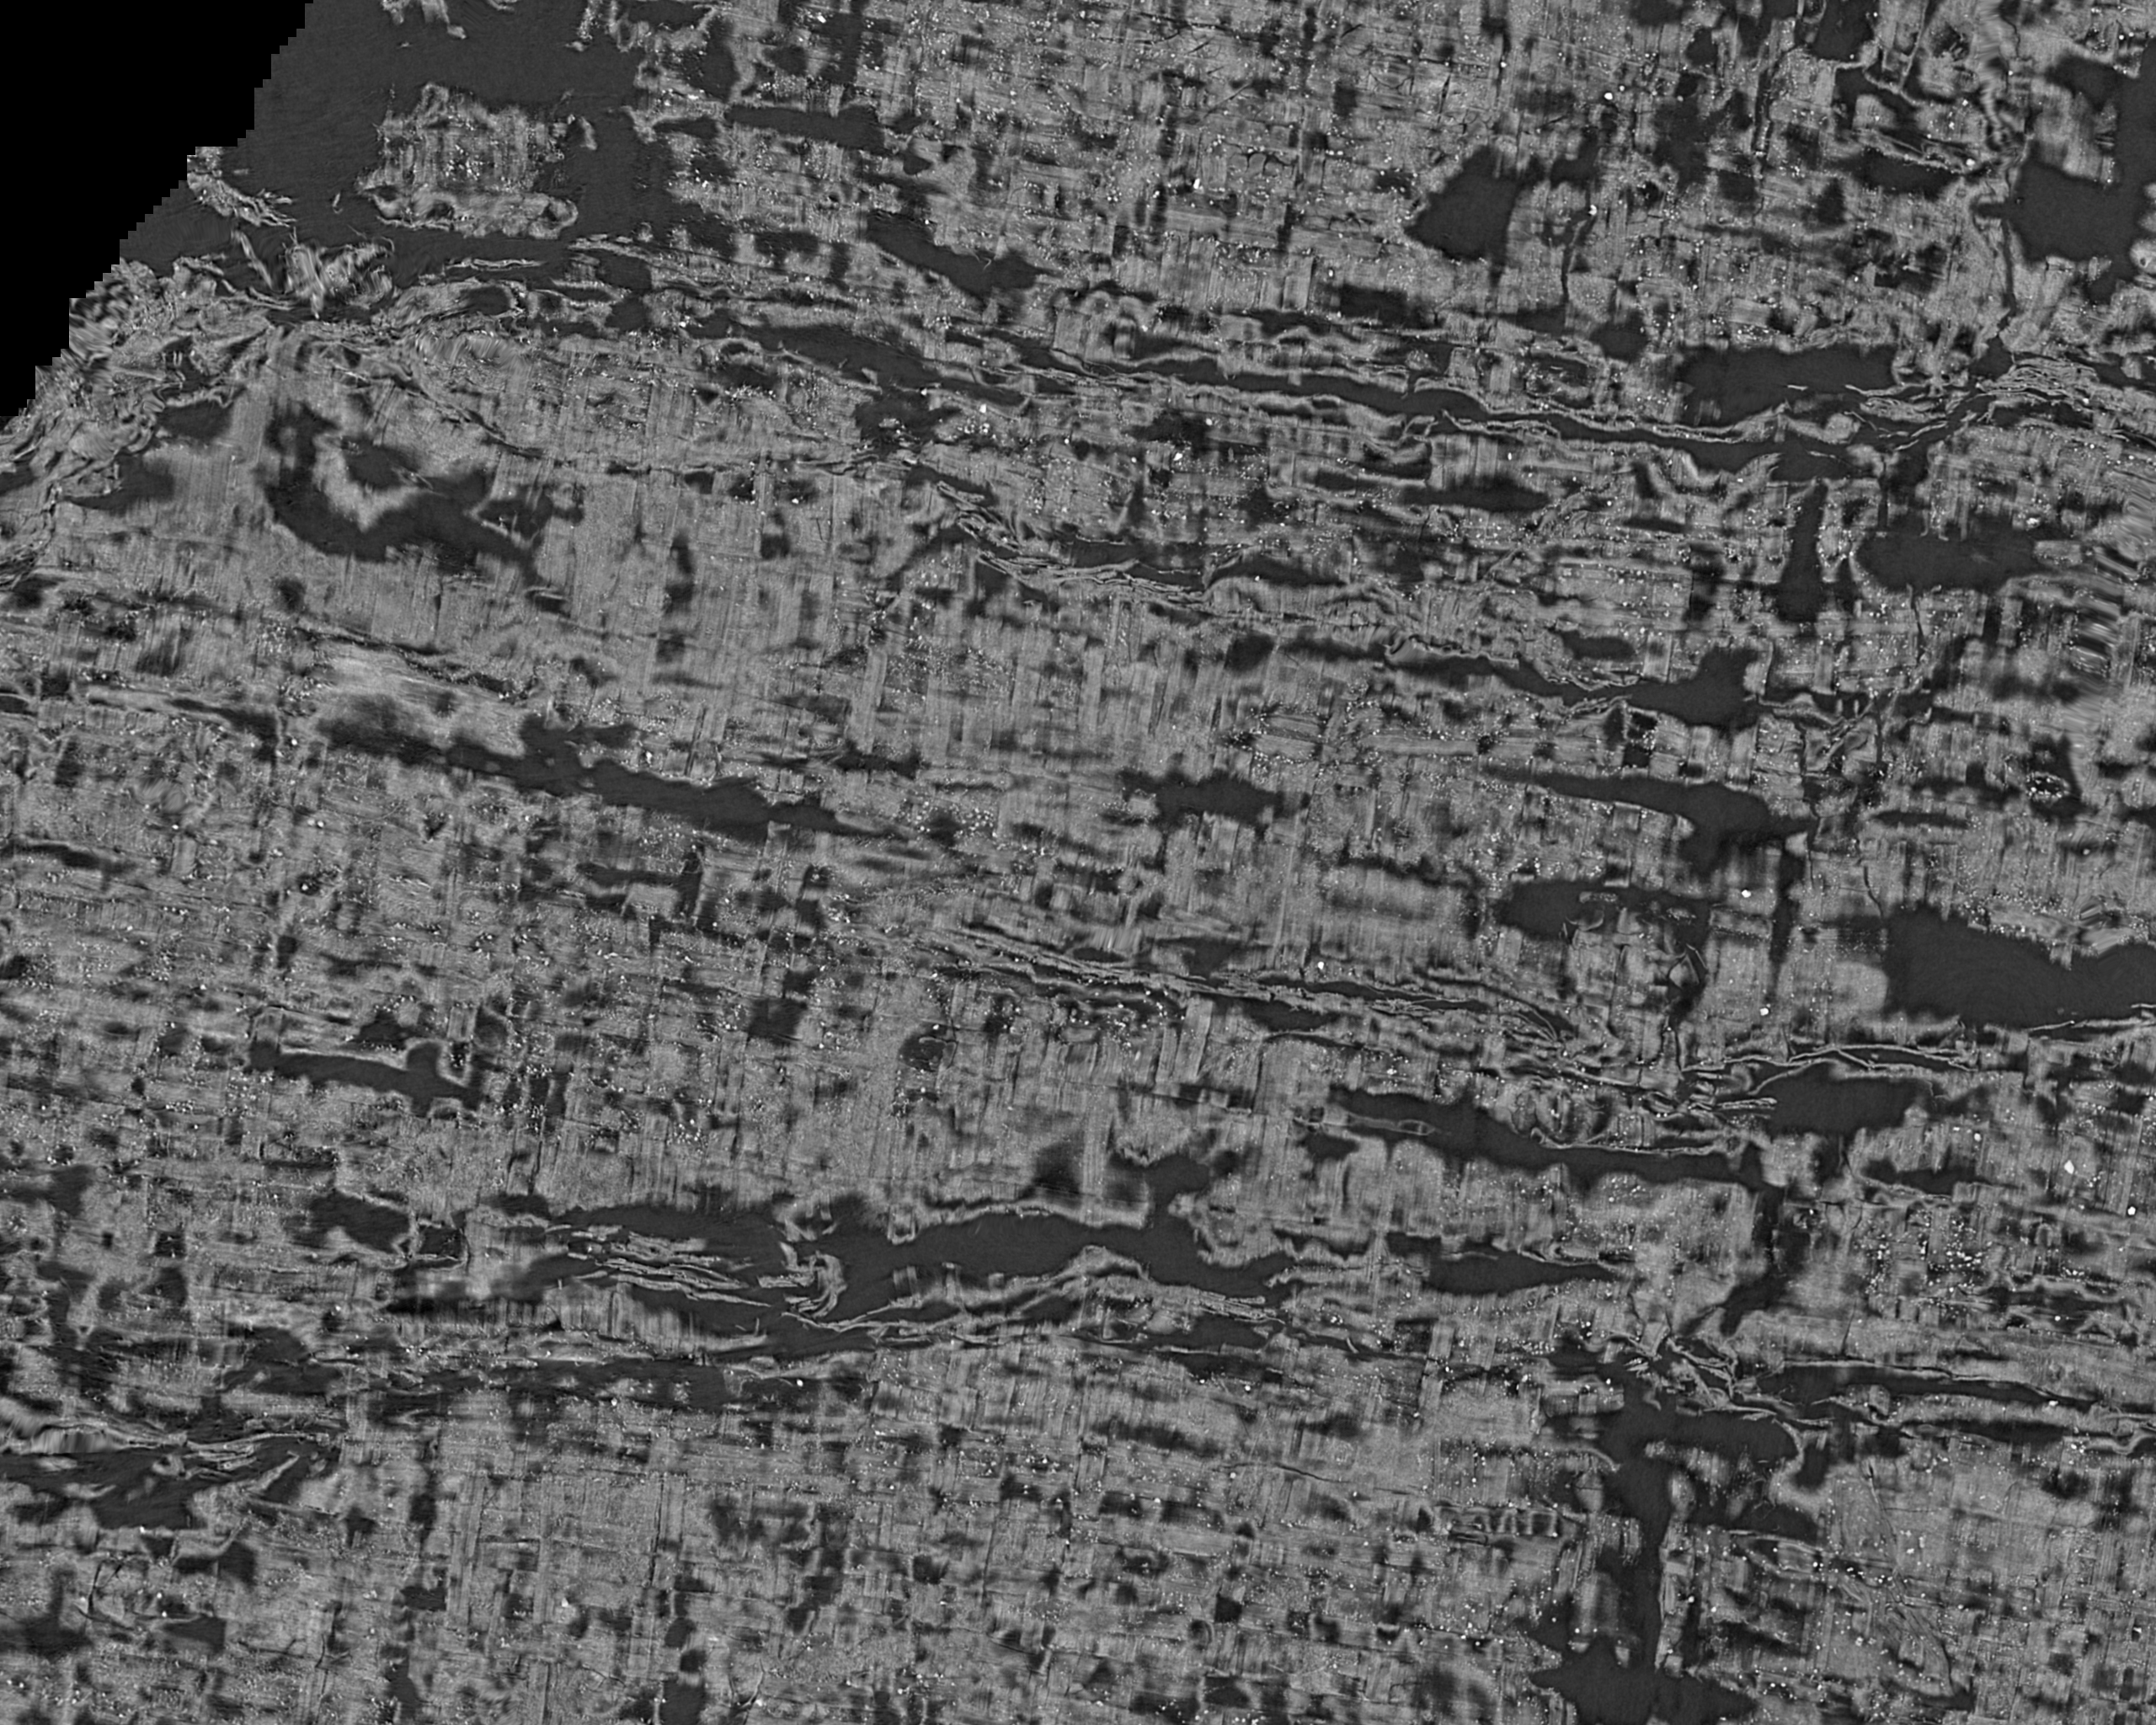
\includegraphics[width=122.48pt]{../figures/ag1/ag1_1_texture.png}}\end{minipage}\hspace{2pt}\begin{minipage}[t]{122.48pt}\centering\href{https://raw.githubusercontent.com/evilaliv3/vesuvius-challenge-pipeline/main/results/db27c806-rectina/src/figures/ag1/ag1_2_labels.png}{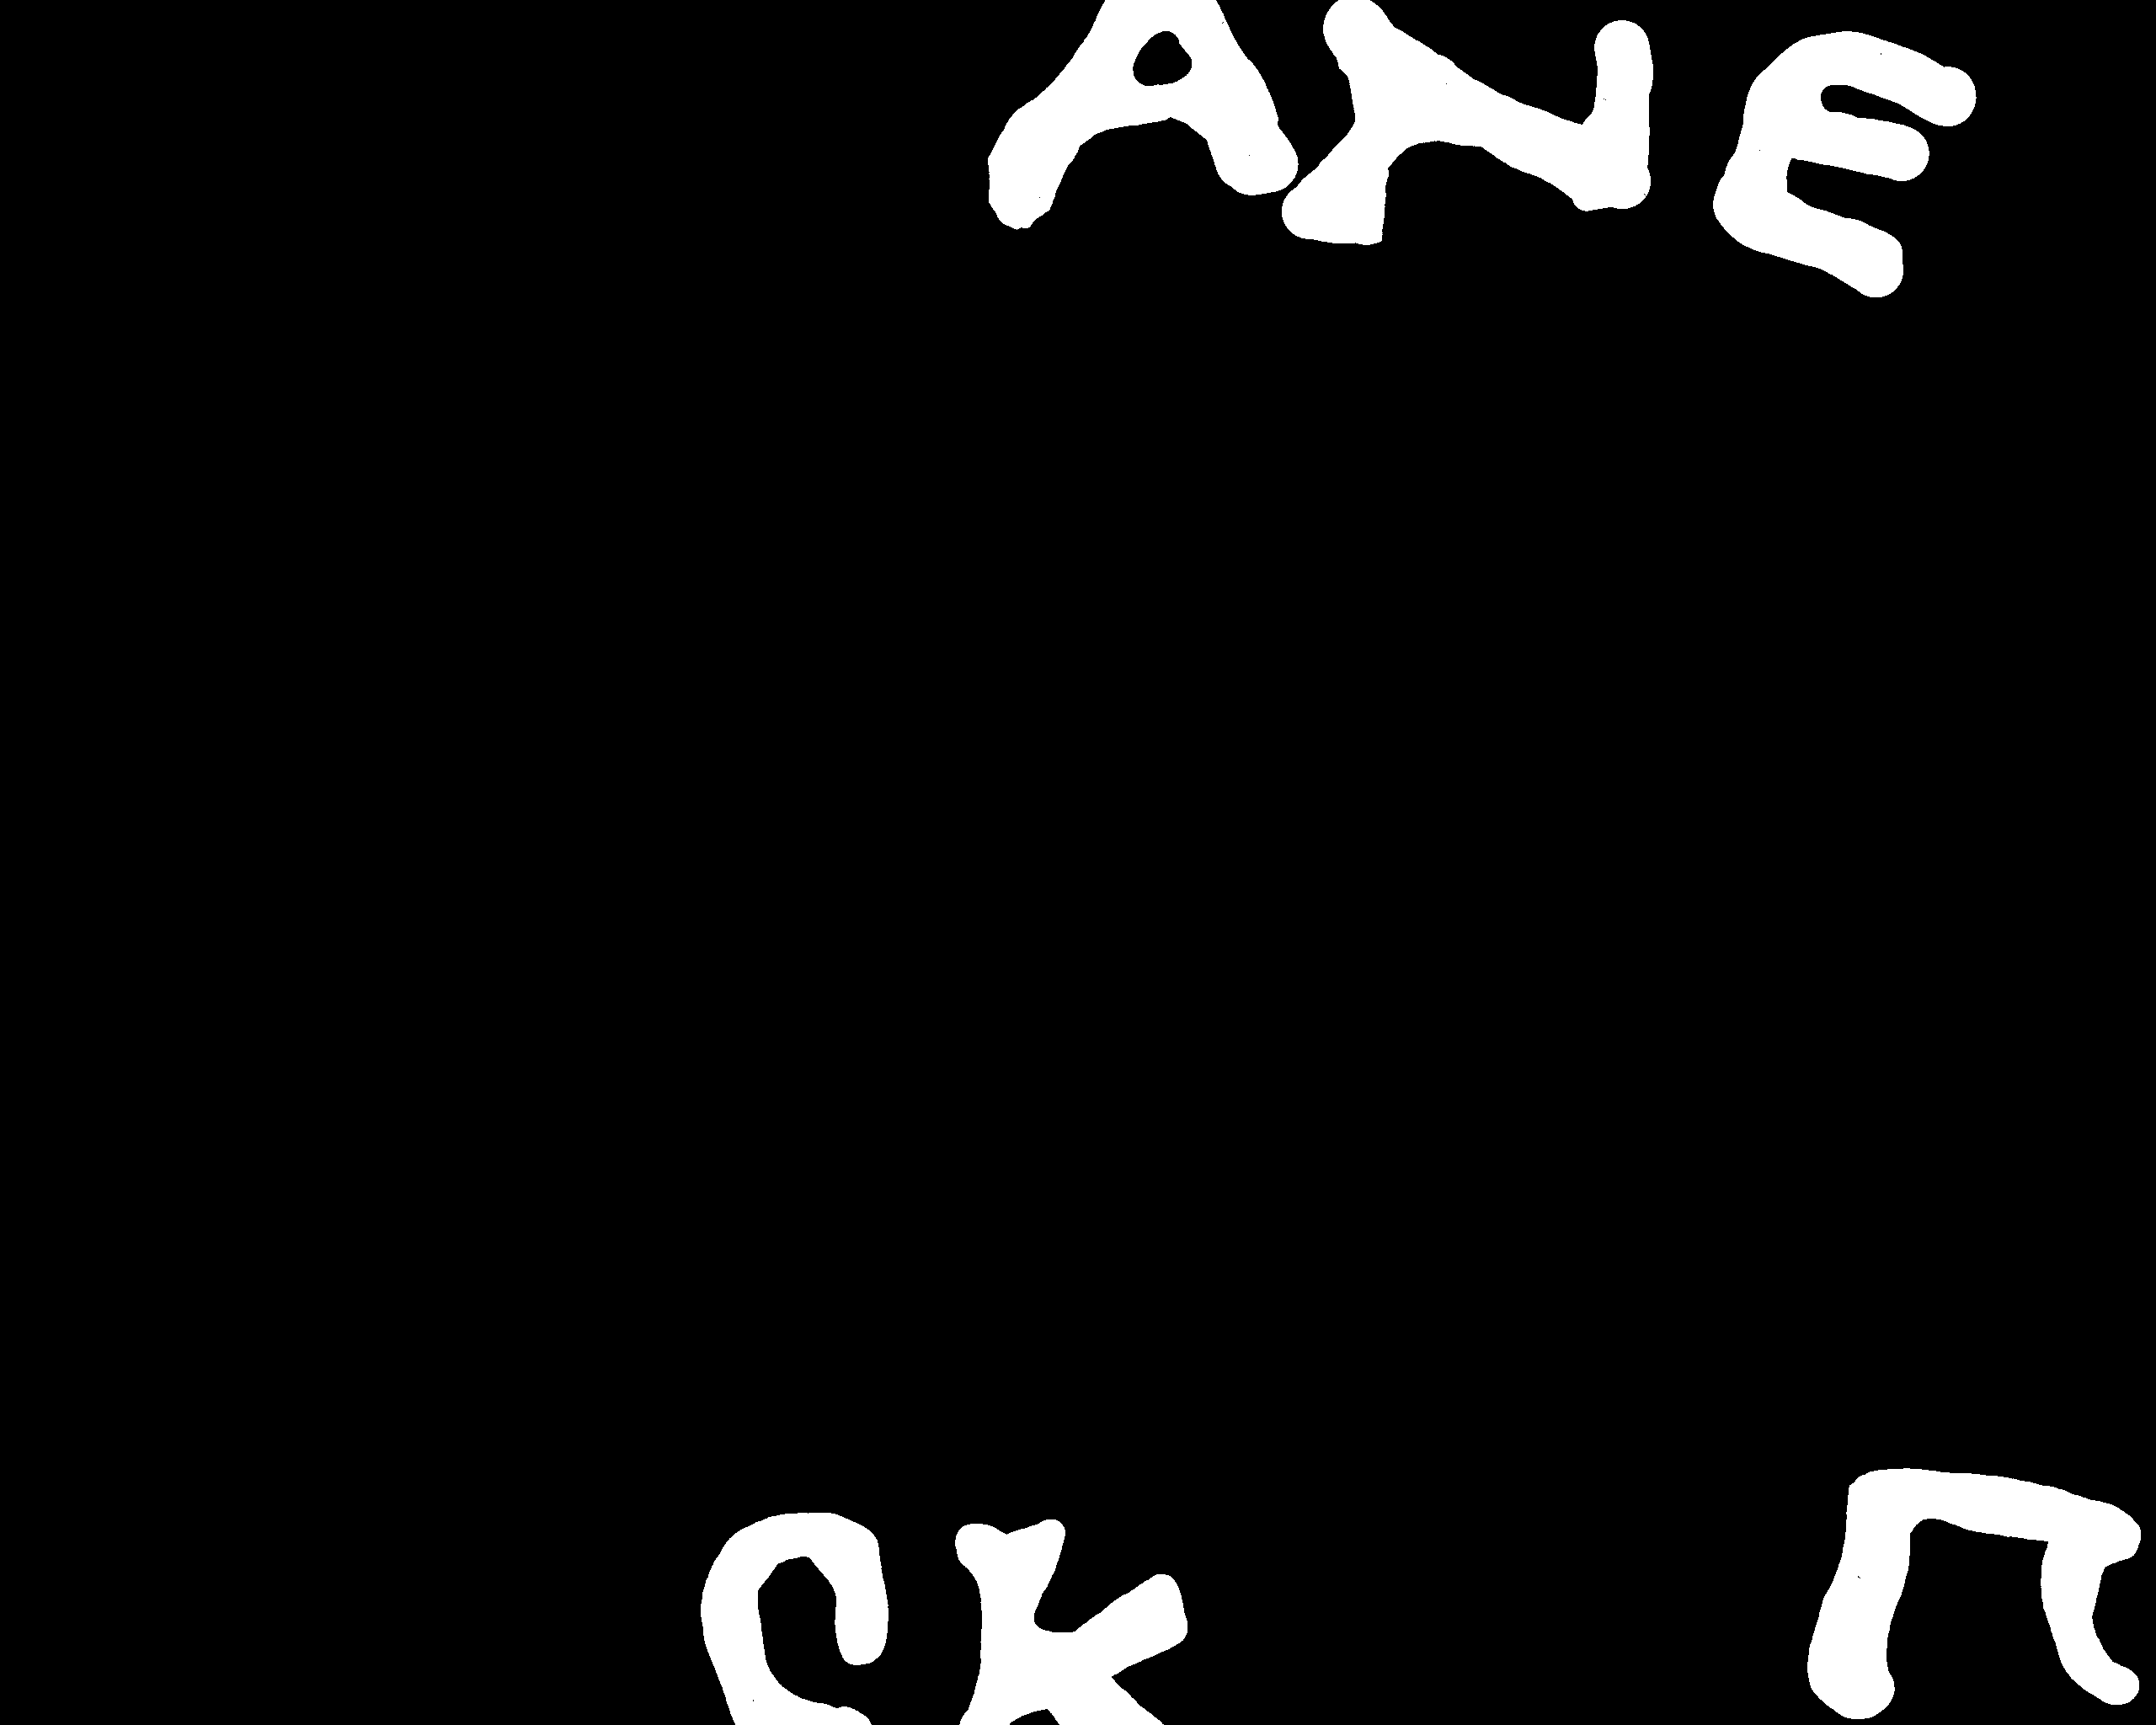
\includegraphics[width=122.48pt]{../figures/ag1/ag1_2_labels.png}}\end{minipage}}
\par\vspace{4pt}
\noindent\makebox[\columnwidth][c]{\begin{minipage}[t]{122.48pt}\centering\href{https://raw.githubusercontent.com/evilaliv3/vesuvius-challenge-pipeline/main/results/db27c806-rectina/src/figures/ag1/ag1_3_reader-v2.png}{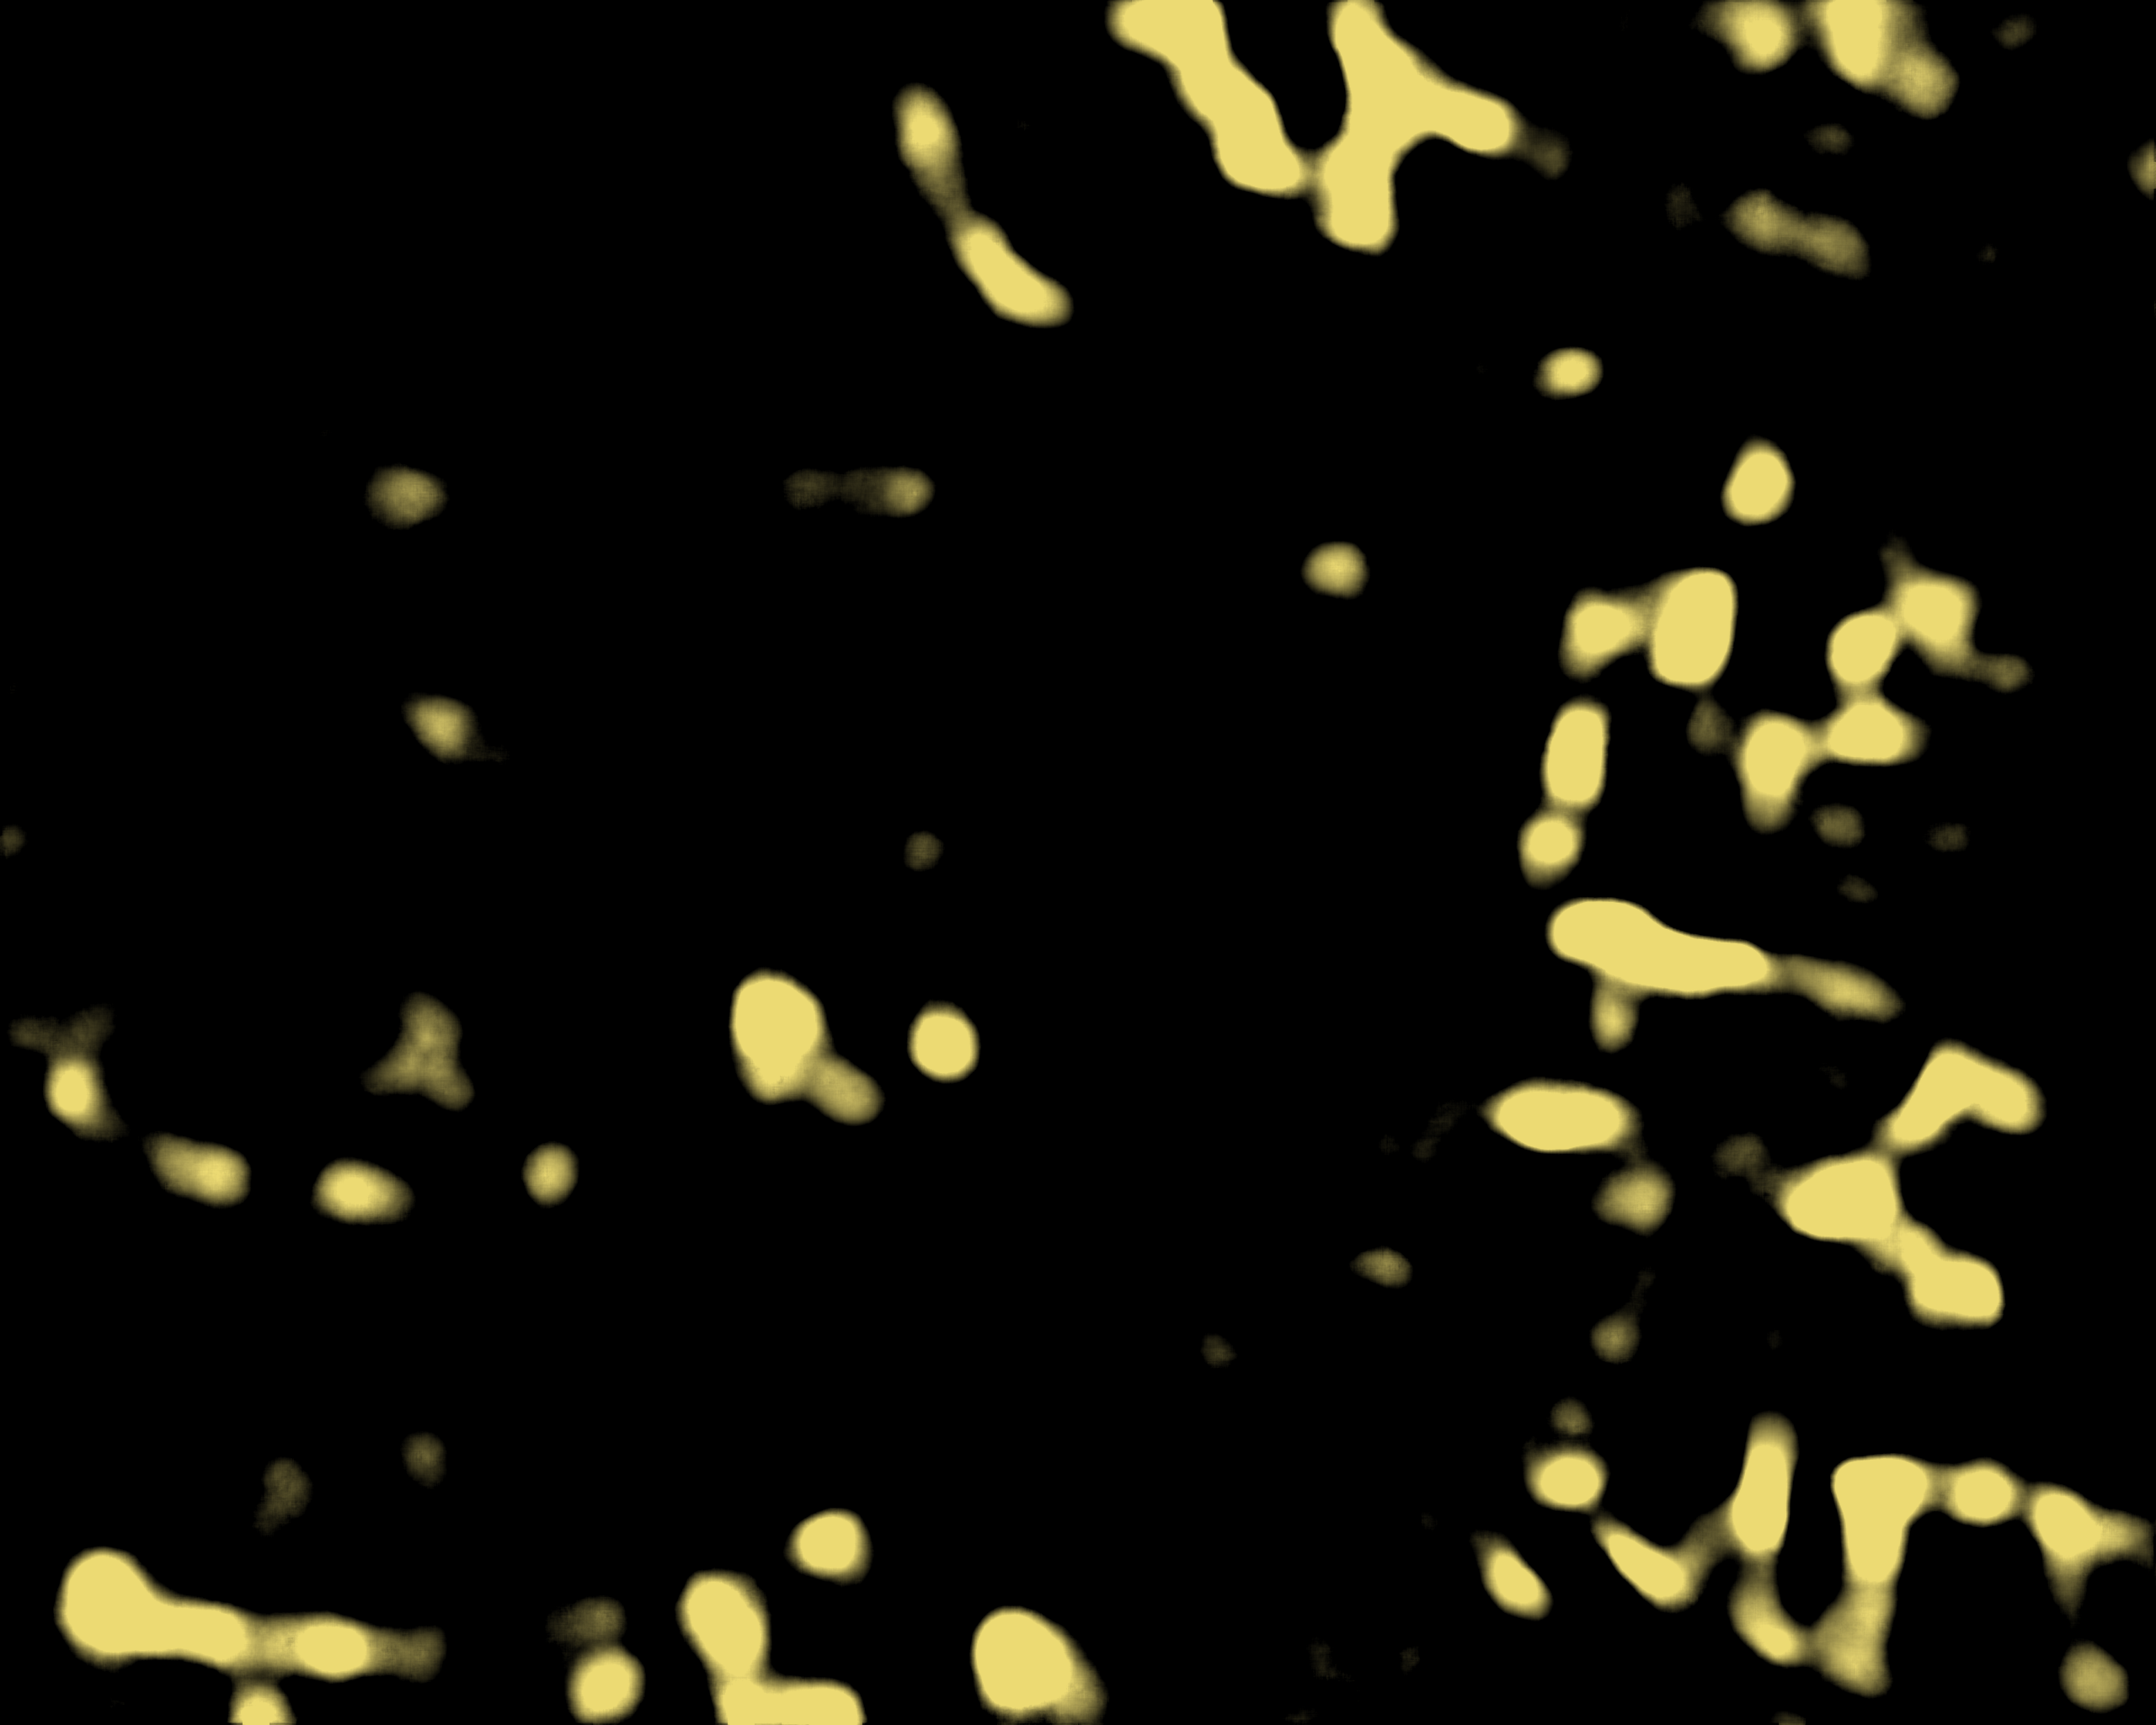
\includegraphics[width=122.48pt]{../figures/ag1/ag1_3_reader-v2.png}}\end{minipage}\hspace{2pt}\begin{minipage}[t]{122.48pt}\centering\href{https://raw.githubusercontent.com/evilaliv3/vesuvius-challenge-pipeline/main/results/db27c806-rectina/src/figures/ag1/ag1_5_rectina-m1.png}{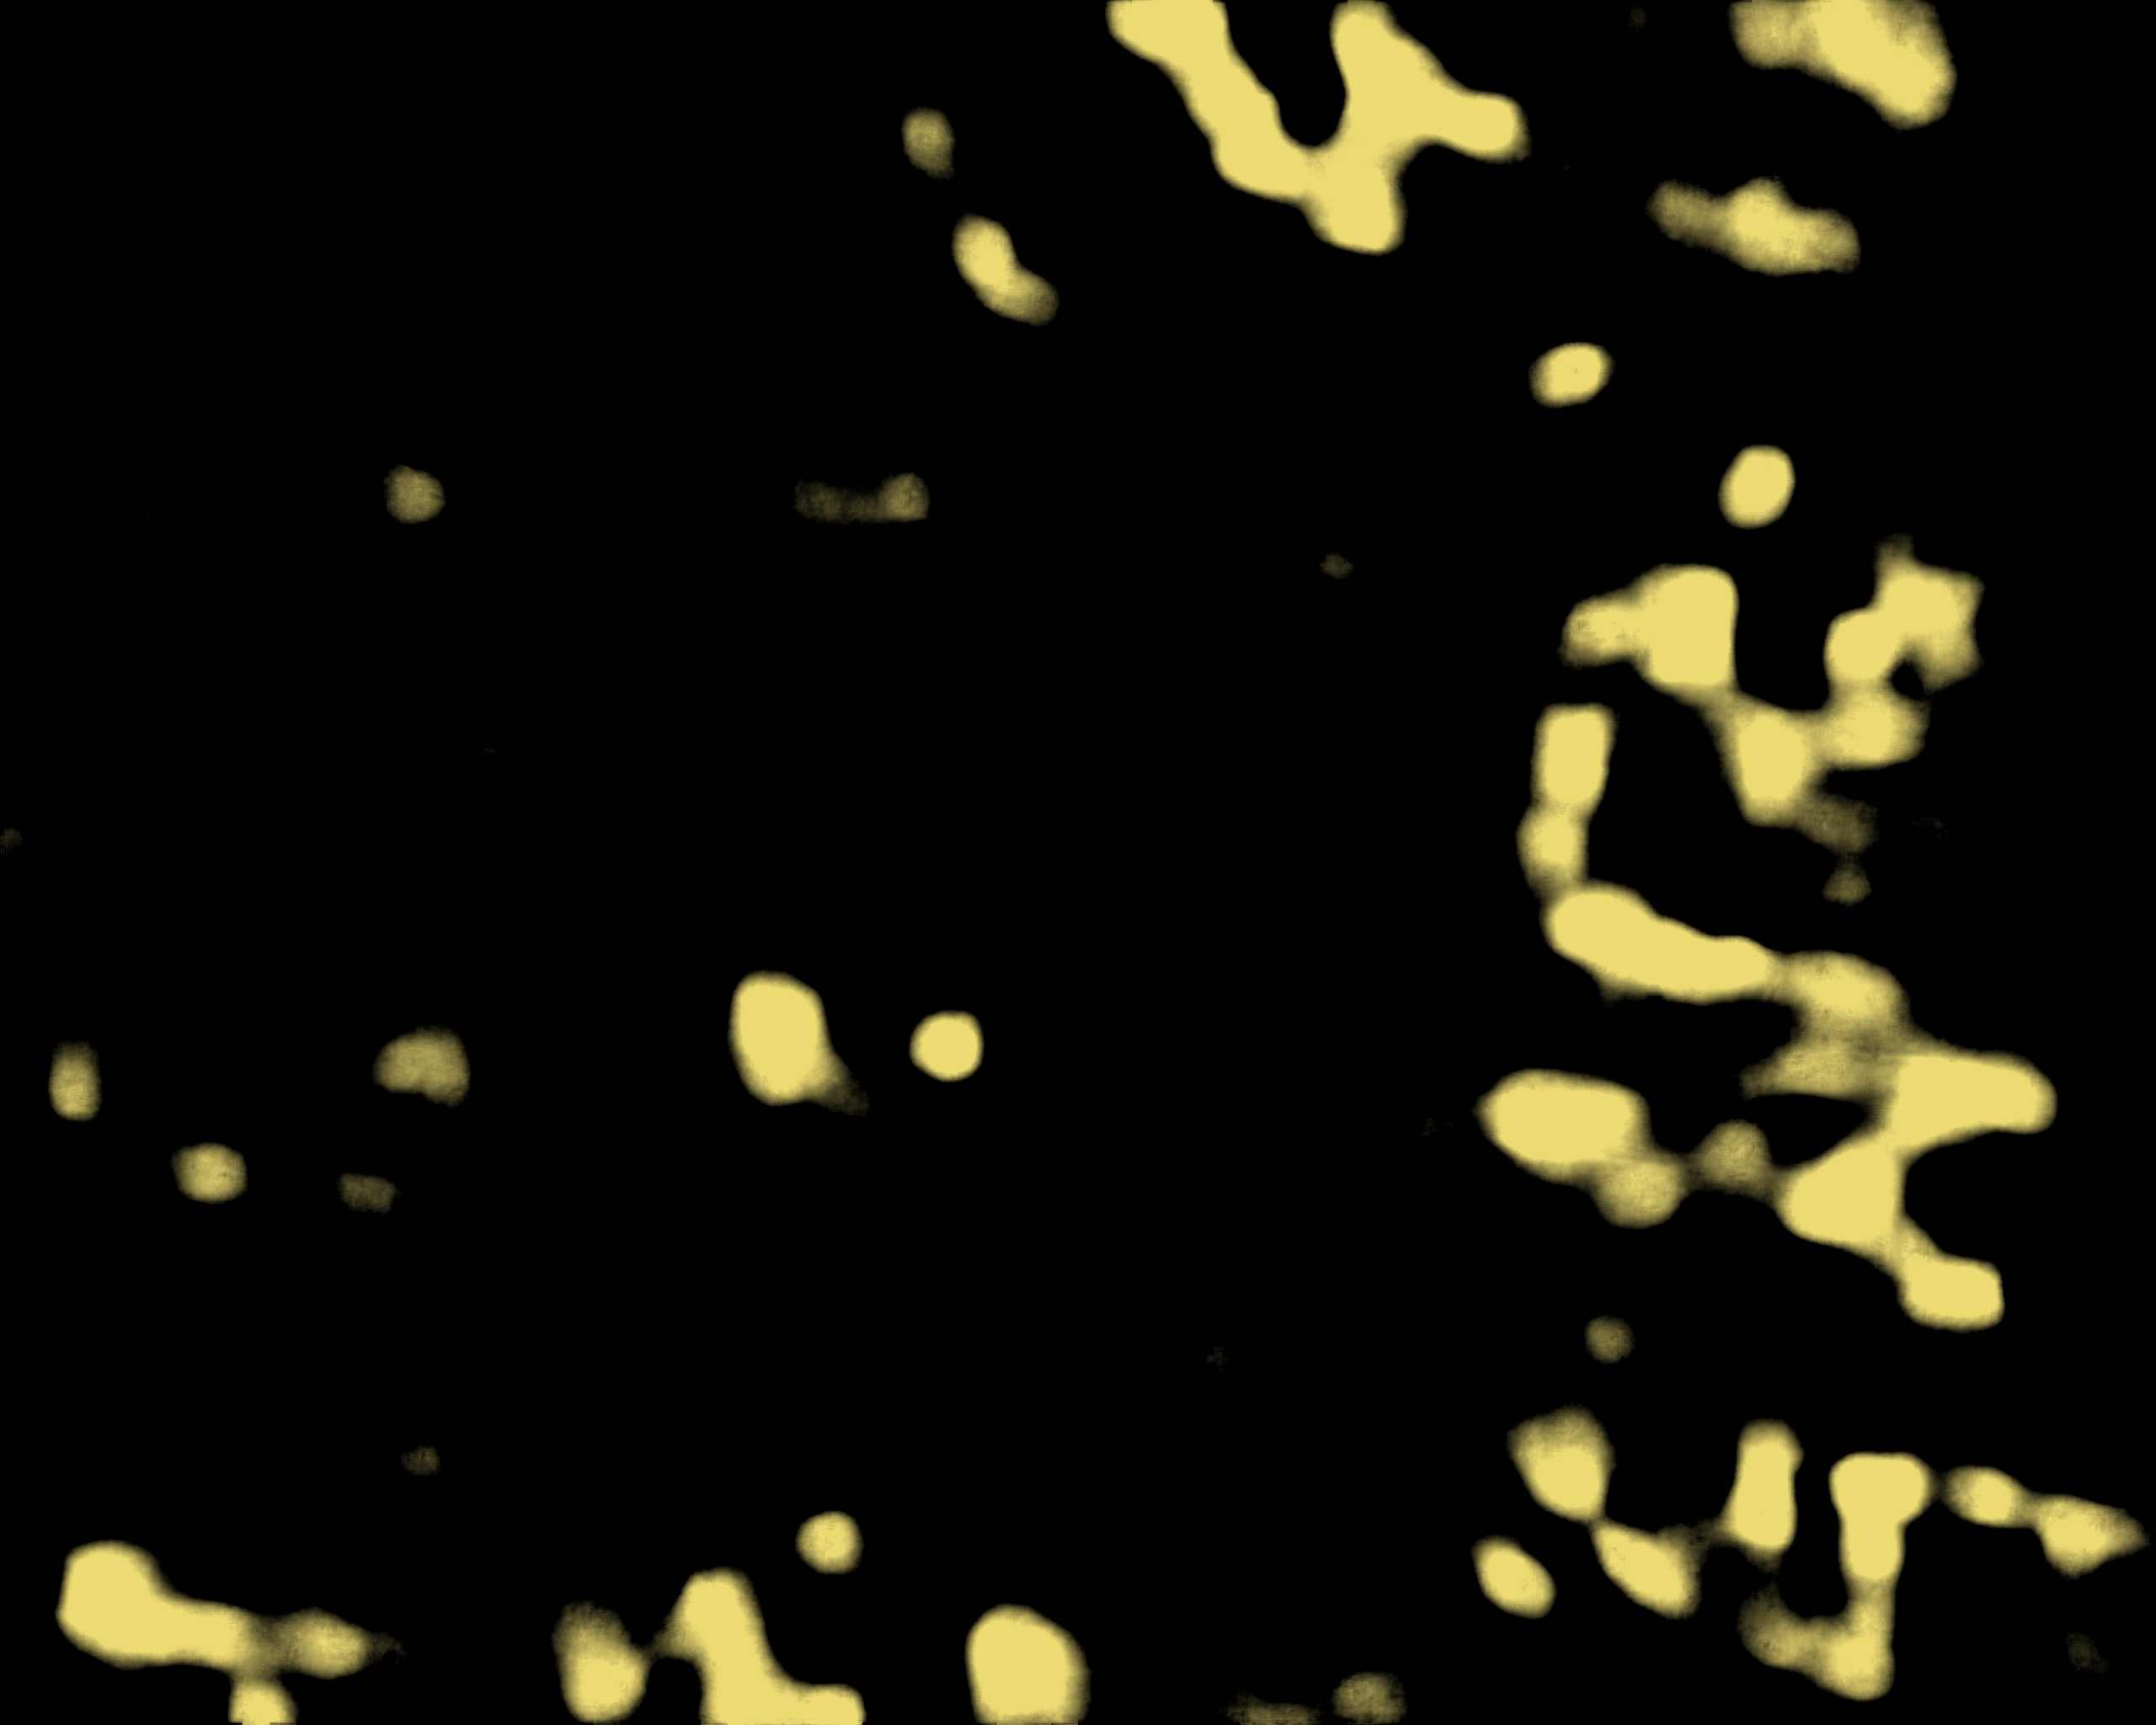
\includegraphics[width=122.48pt]{../figures/ag1/ag1_5_rectina-m1.png}}\end{minipage}}
\par\vspace{4pt}
\noindent\makebox[\columnwidth][c]{\begin{minipage}[t]{122.48pt}\centering\href{https://raw.githubusercontent.com/evilaliv3/vesuvius-challenge-pipeline/main/results/db27c806-rectina/src/figures/ag1/ag1_4_reader-v3.png}{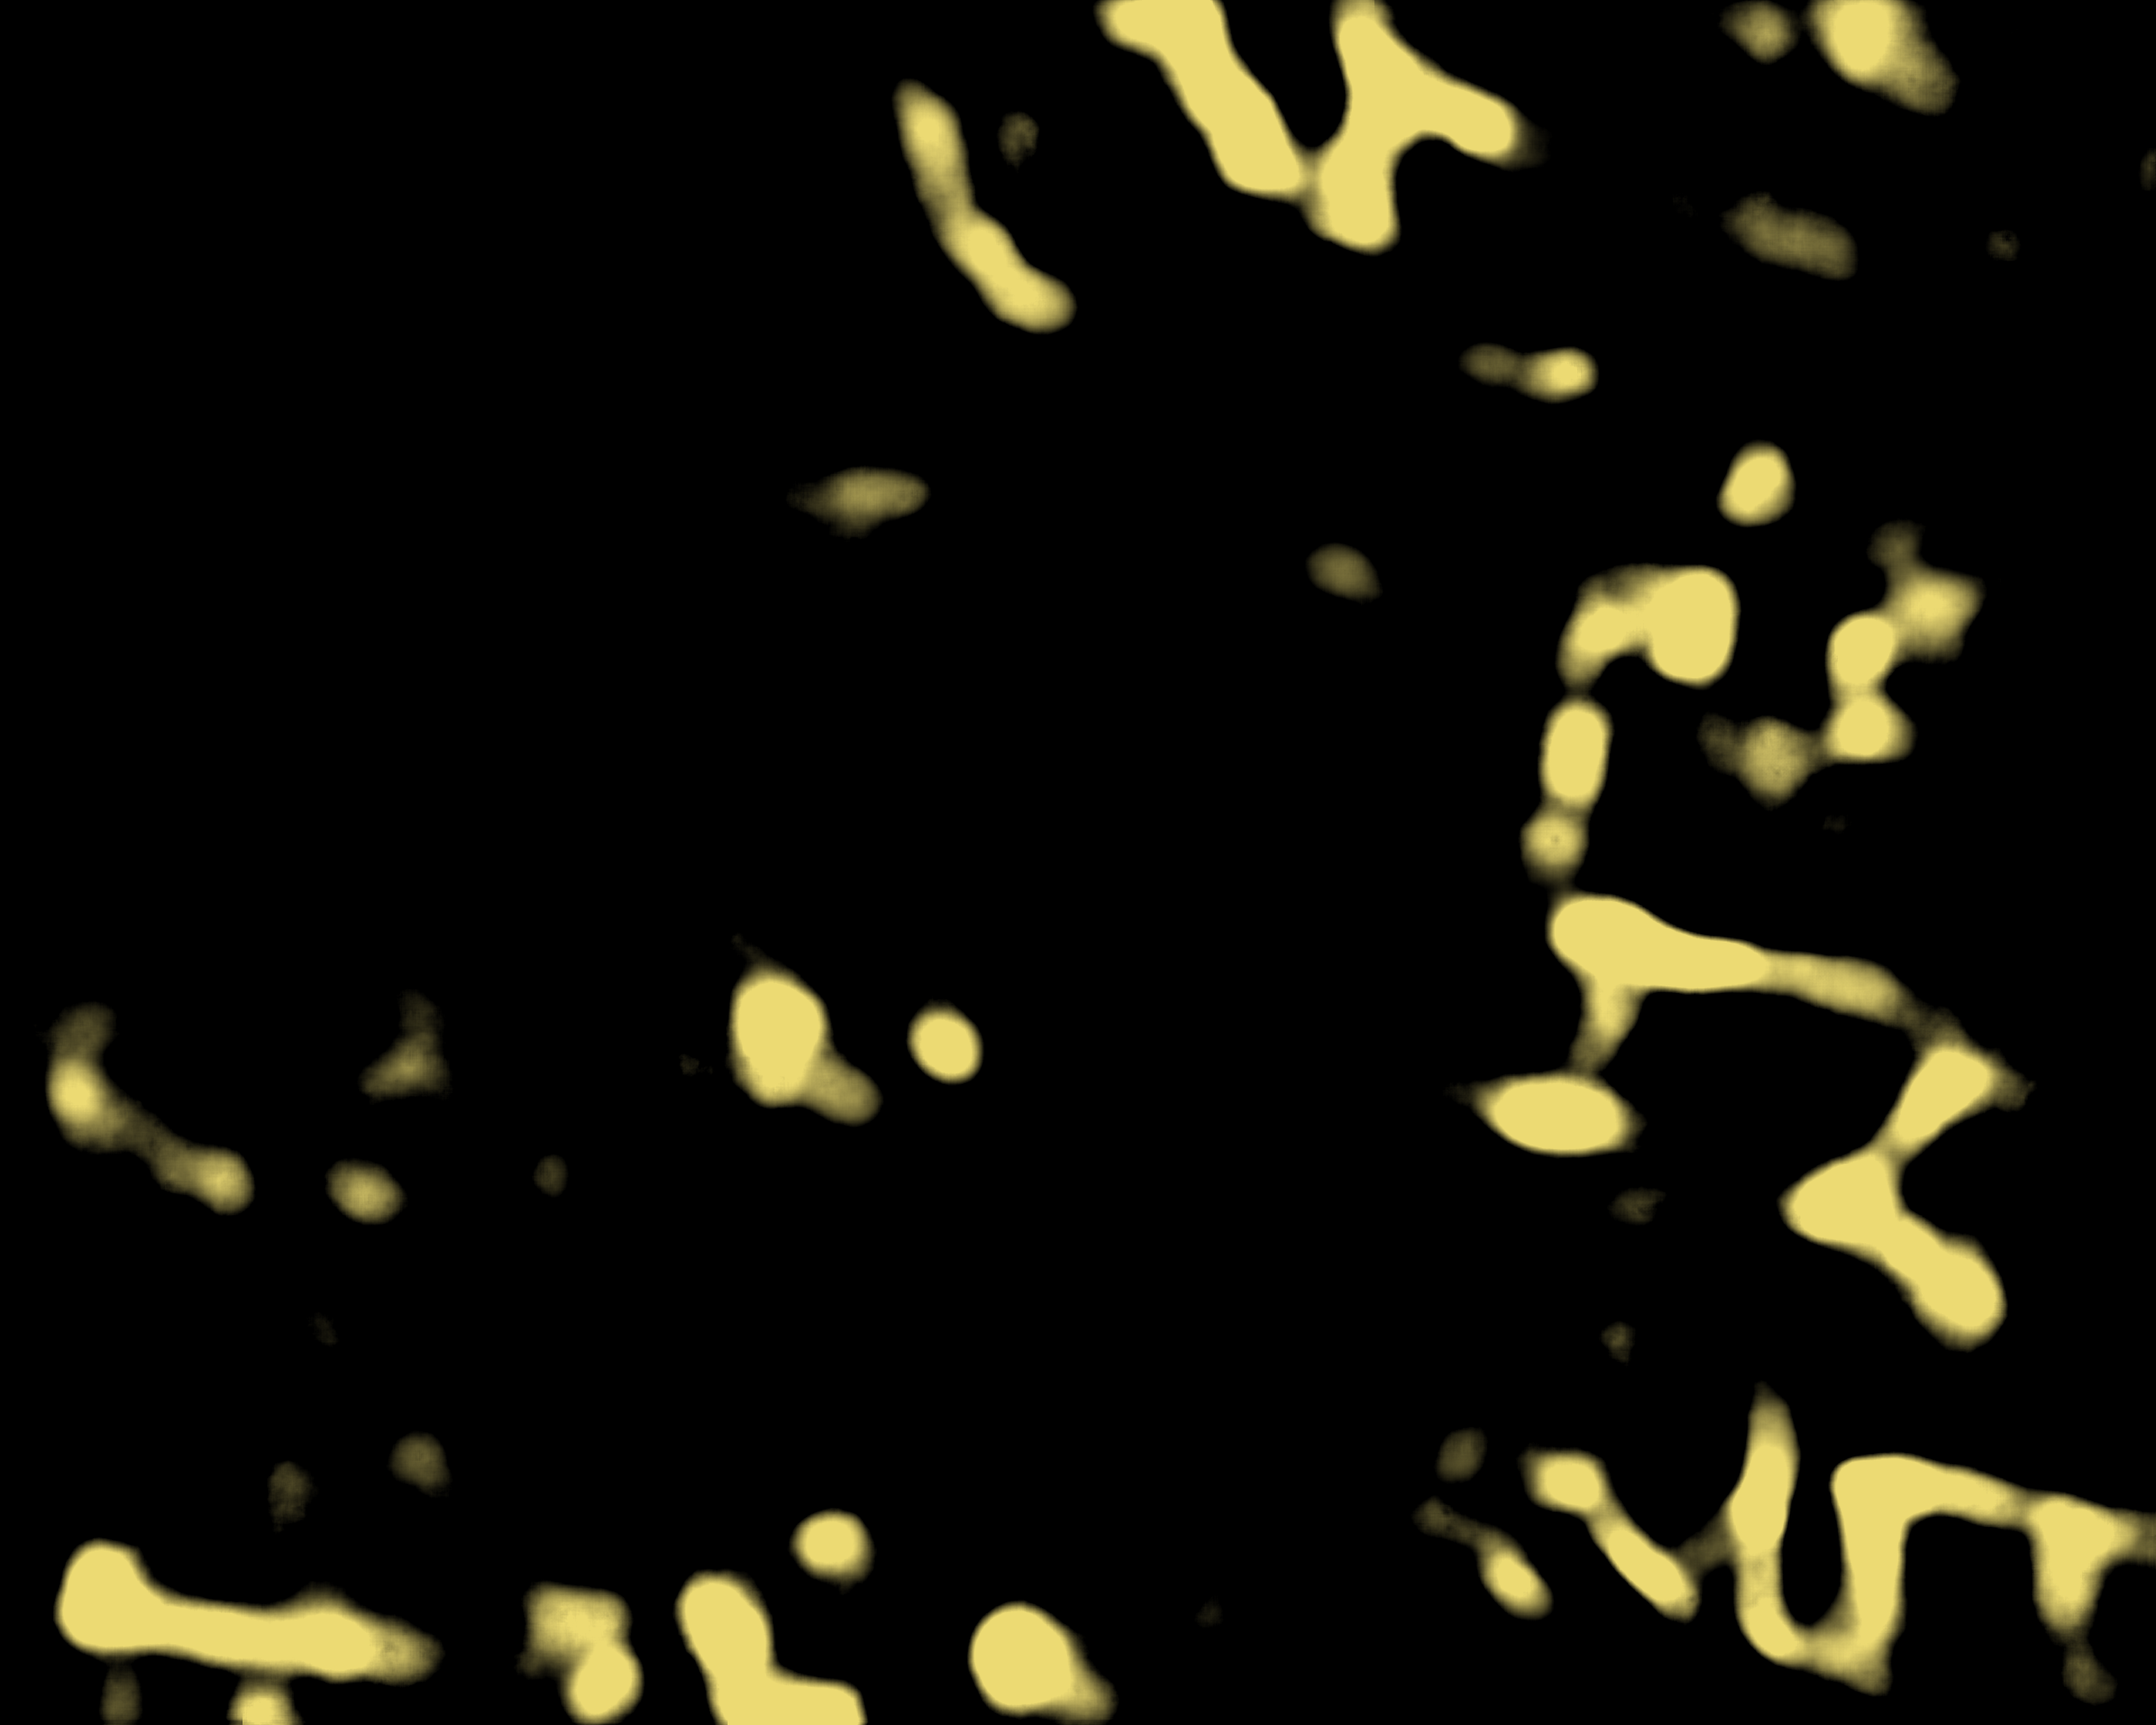
\includegraphics[width=122.48pt]{../figures/ag1/ag1_4_reader-v3.png}}\end{minipage}\hspace{2pt}\begin{minipage}[t]{122.48pt}\centering\href{https://raw.githubusercontent.com/evilaliv3/vesuvius-challenge-pipeline/main/results/db27c806-rectina/src/figures/ag1/ag1_6_rectina-m2.png}{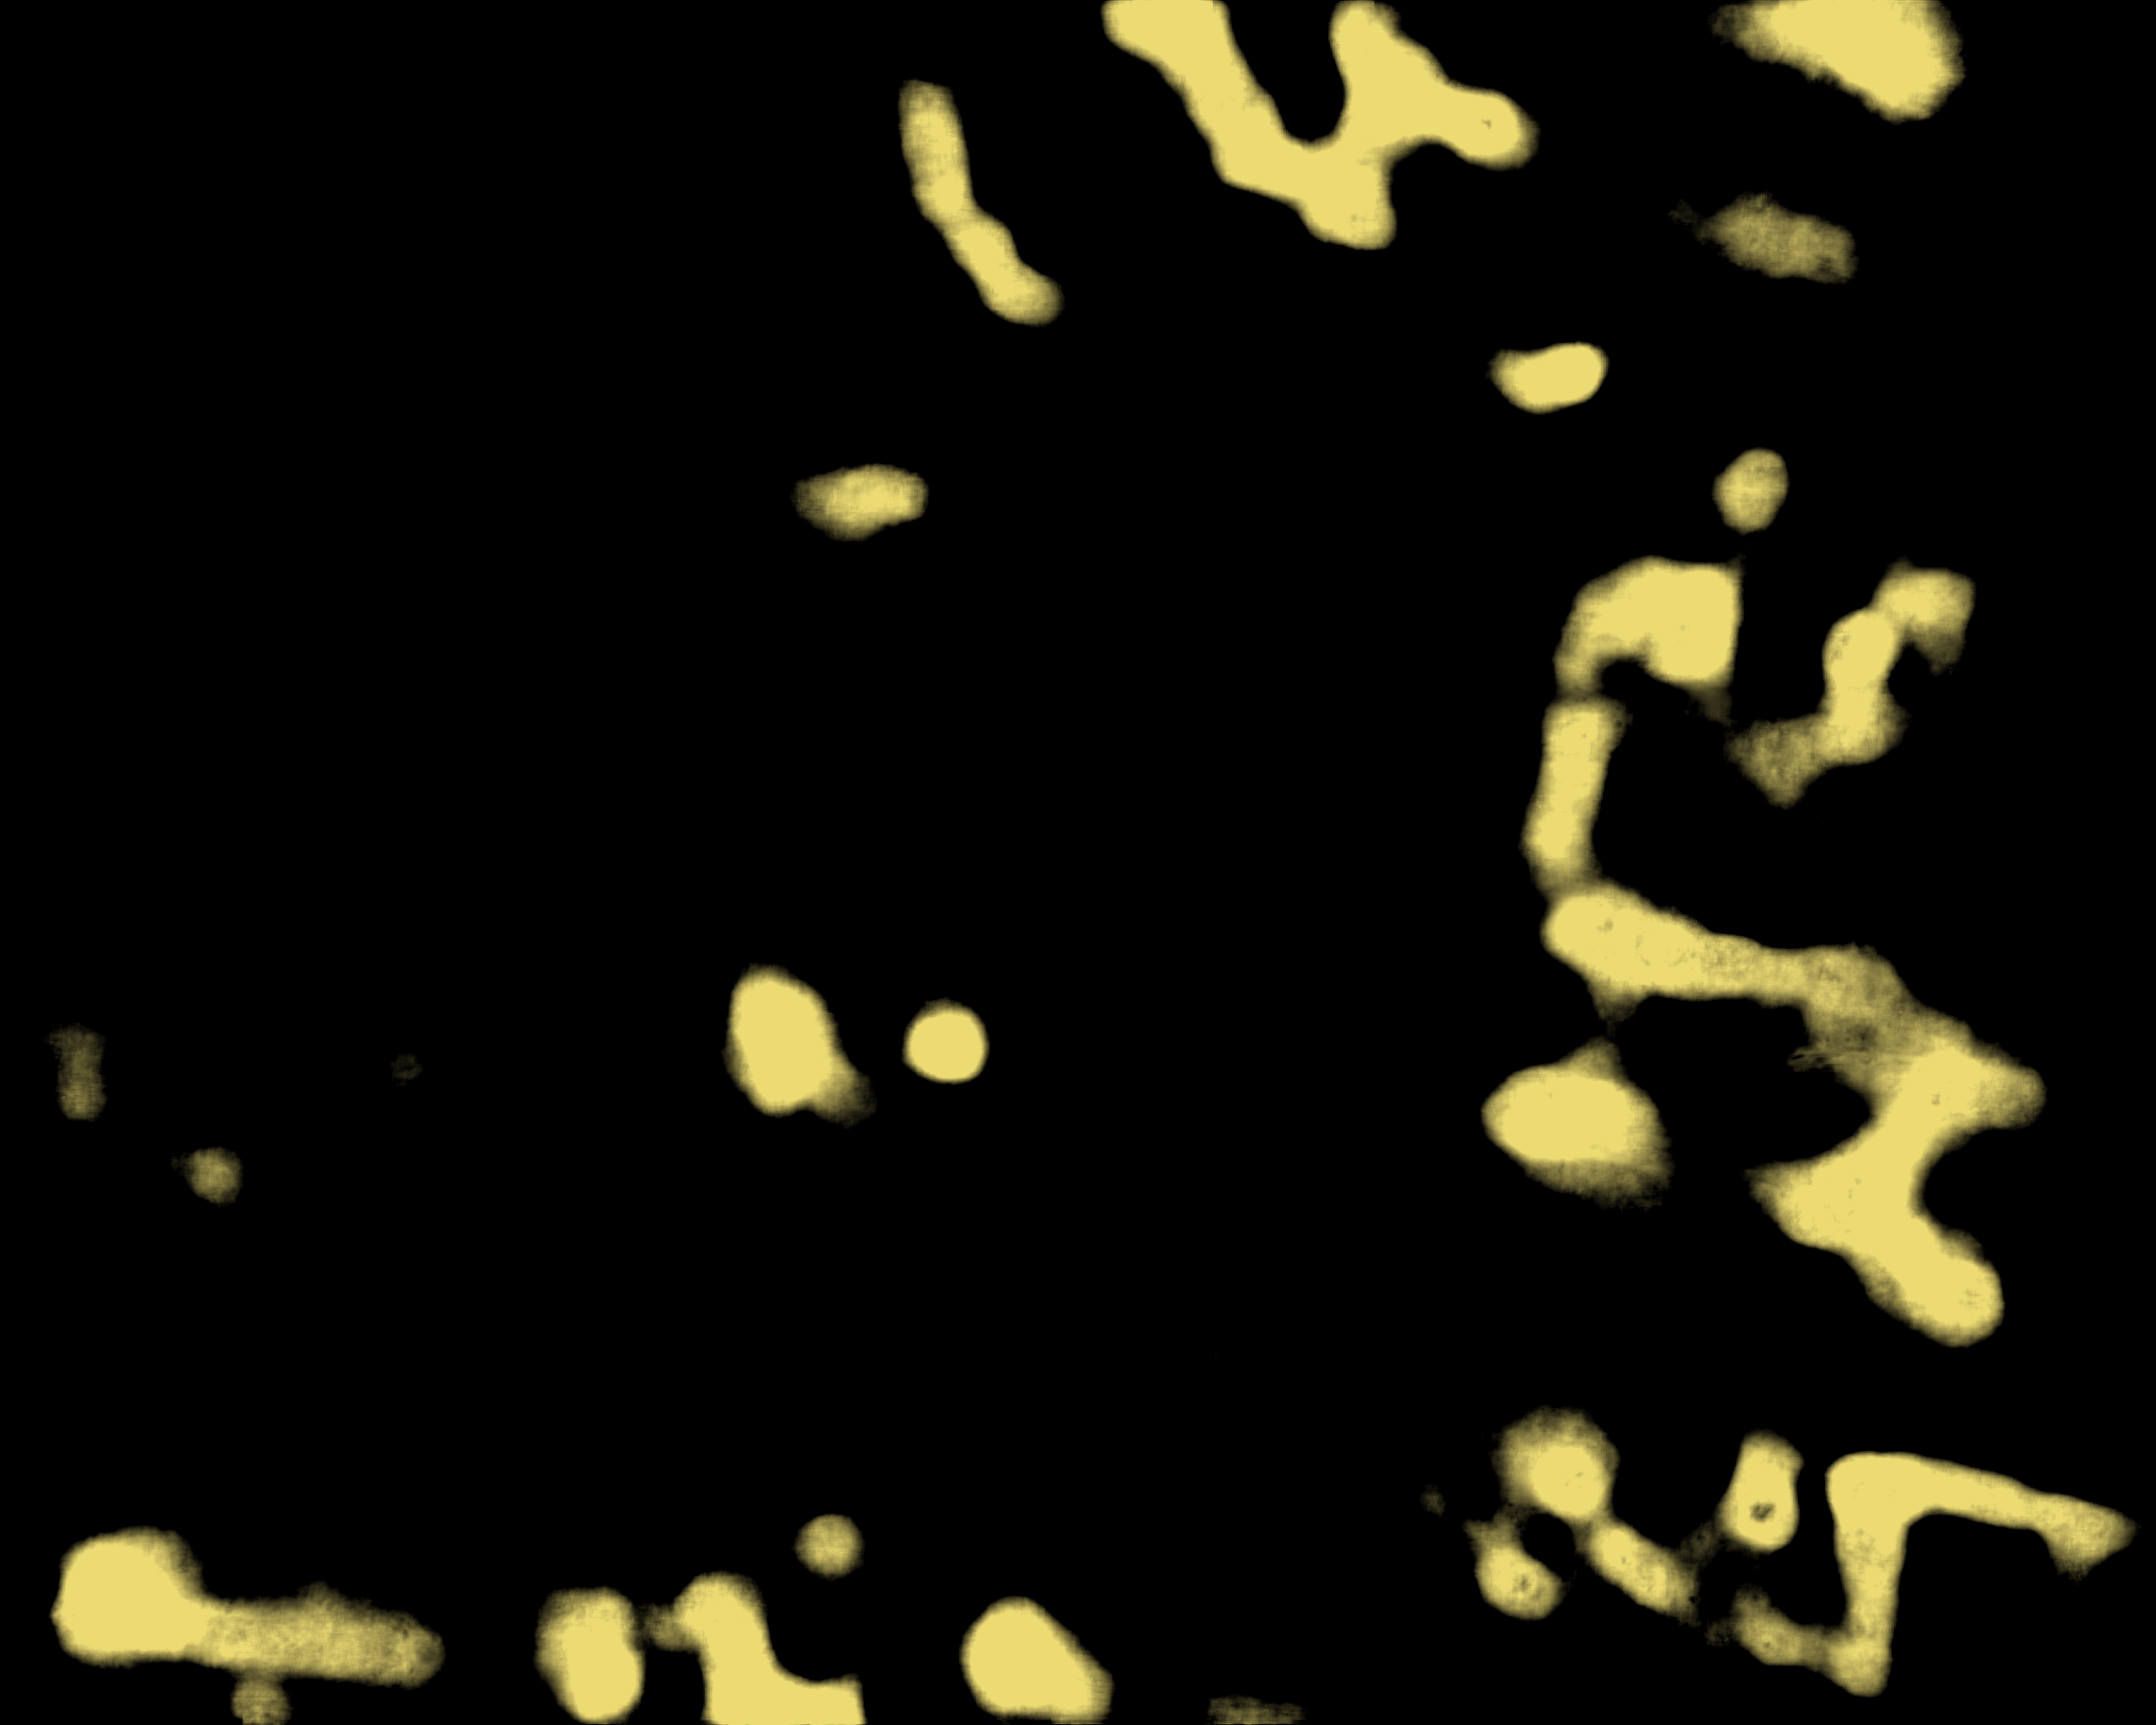
\includegraphics[width=122.48pt]{../figures/ag1/ag1_6_rectina-m2.png}}\end{minipage}}
\caption{Control unit 0841 ag1, three rows of two panels. Row 1: left, Texture; right, Labels. Row 2: left, Reader v2; right, Rectina m1 (display windows: Reader v2 0.447222 to 0.621051 (ramp); Rectina m1 0.623262 to 0.741702 (ramp)). Row 3: left, Reader v3; right, Rectina m2 (display windows: Reader v3 0.470294 to 0.693186 (ramp); Rectina m2 0.671638 to 0.774498 (ramp)). Each map is stretched between its own percentiles. Reader and model stand side by side in the rows 2 and 3.}
\end{figure}

\begin{figure}[!tbp]
\centering
\noindent\makebox[\columnwidth][c]{\begin{minipage}[t]{122.48pt}\centering\href{https://raw.githubusercontent.com/evilaliv3/vesuvius-challenge-pipeline/main/results/db27c806-rectina/src/figures/ag2/ag2_1_texture.png}{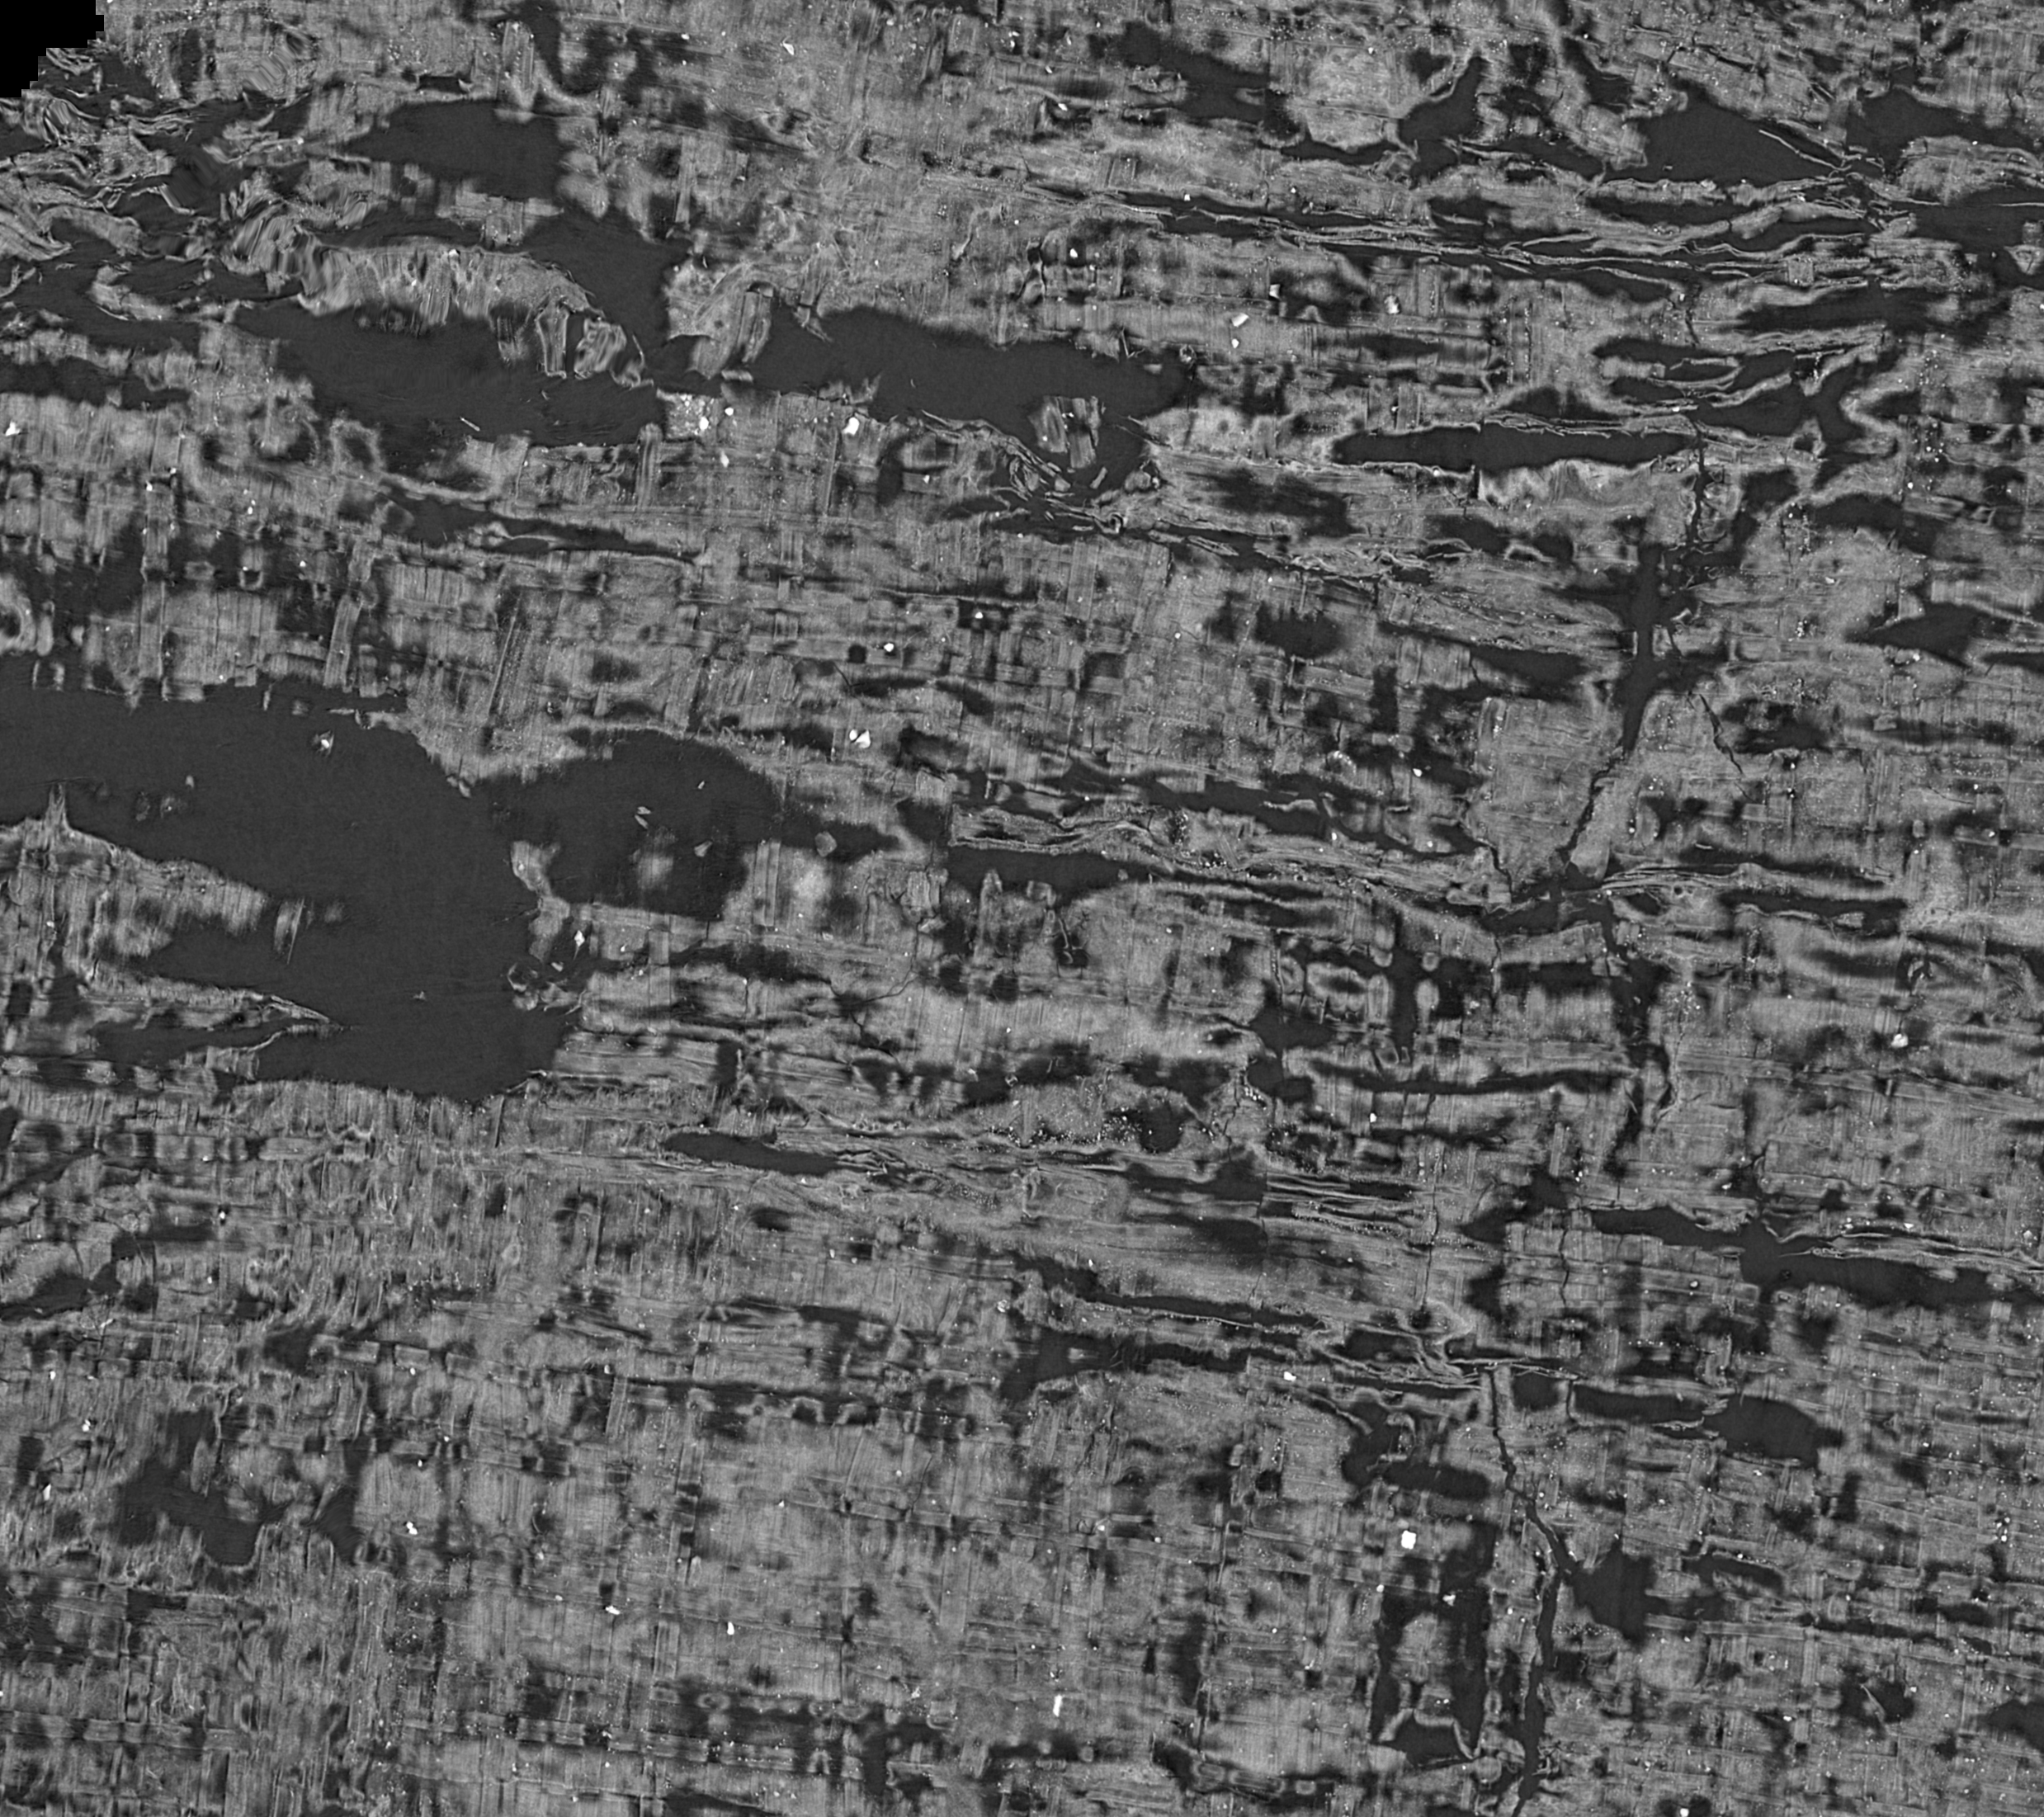
\includegraphics[width=122.48pt]{../figures/ag2/ag2_1_texture.png}}\end{minipage}\hspace{2pt}\begin{minipage}[t]{122.48pt}\centering\href{https://raw.githubusercontent.com/evilaliv3/vesuvius-challenge-pipeline/main/results/db27c806-rectina/src/figures/ag2/ag2_2_labels.png}{
\includegraphics[width=122.48pt]{../figures/ag2/ag2_2_labels.png}}\end{minipage}}
\par\vspace{4pt}
\noindent\makebox[\columnwidth][c]{\begin{minipage}[t]{122.48pt}\centering\href{https://raw.githubusercontent.com/evilaliv3/vesuvius-challenge-pipeline/main/results/db27c806-rectina/src/figures/ag2/ag2_3_reader-v2.png}{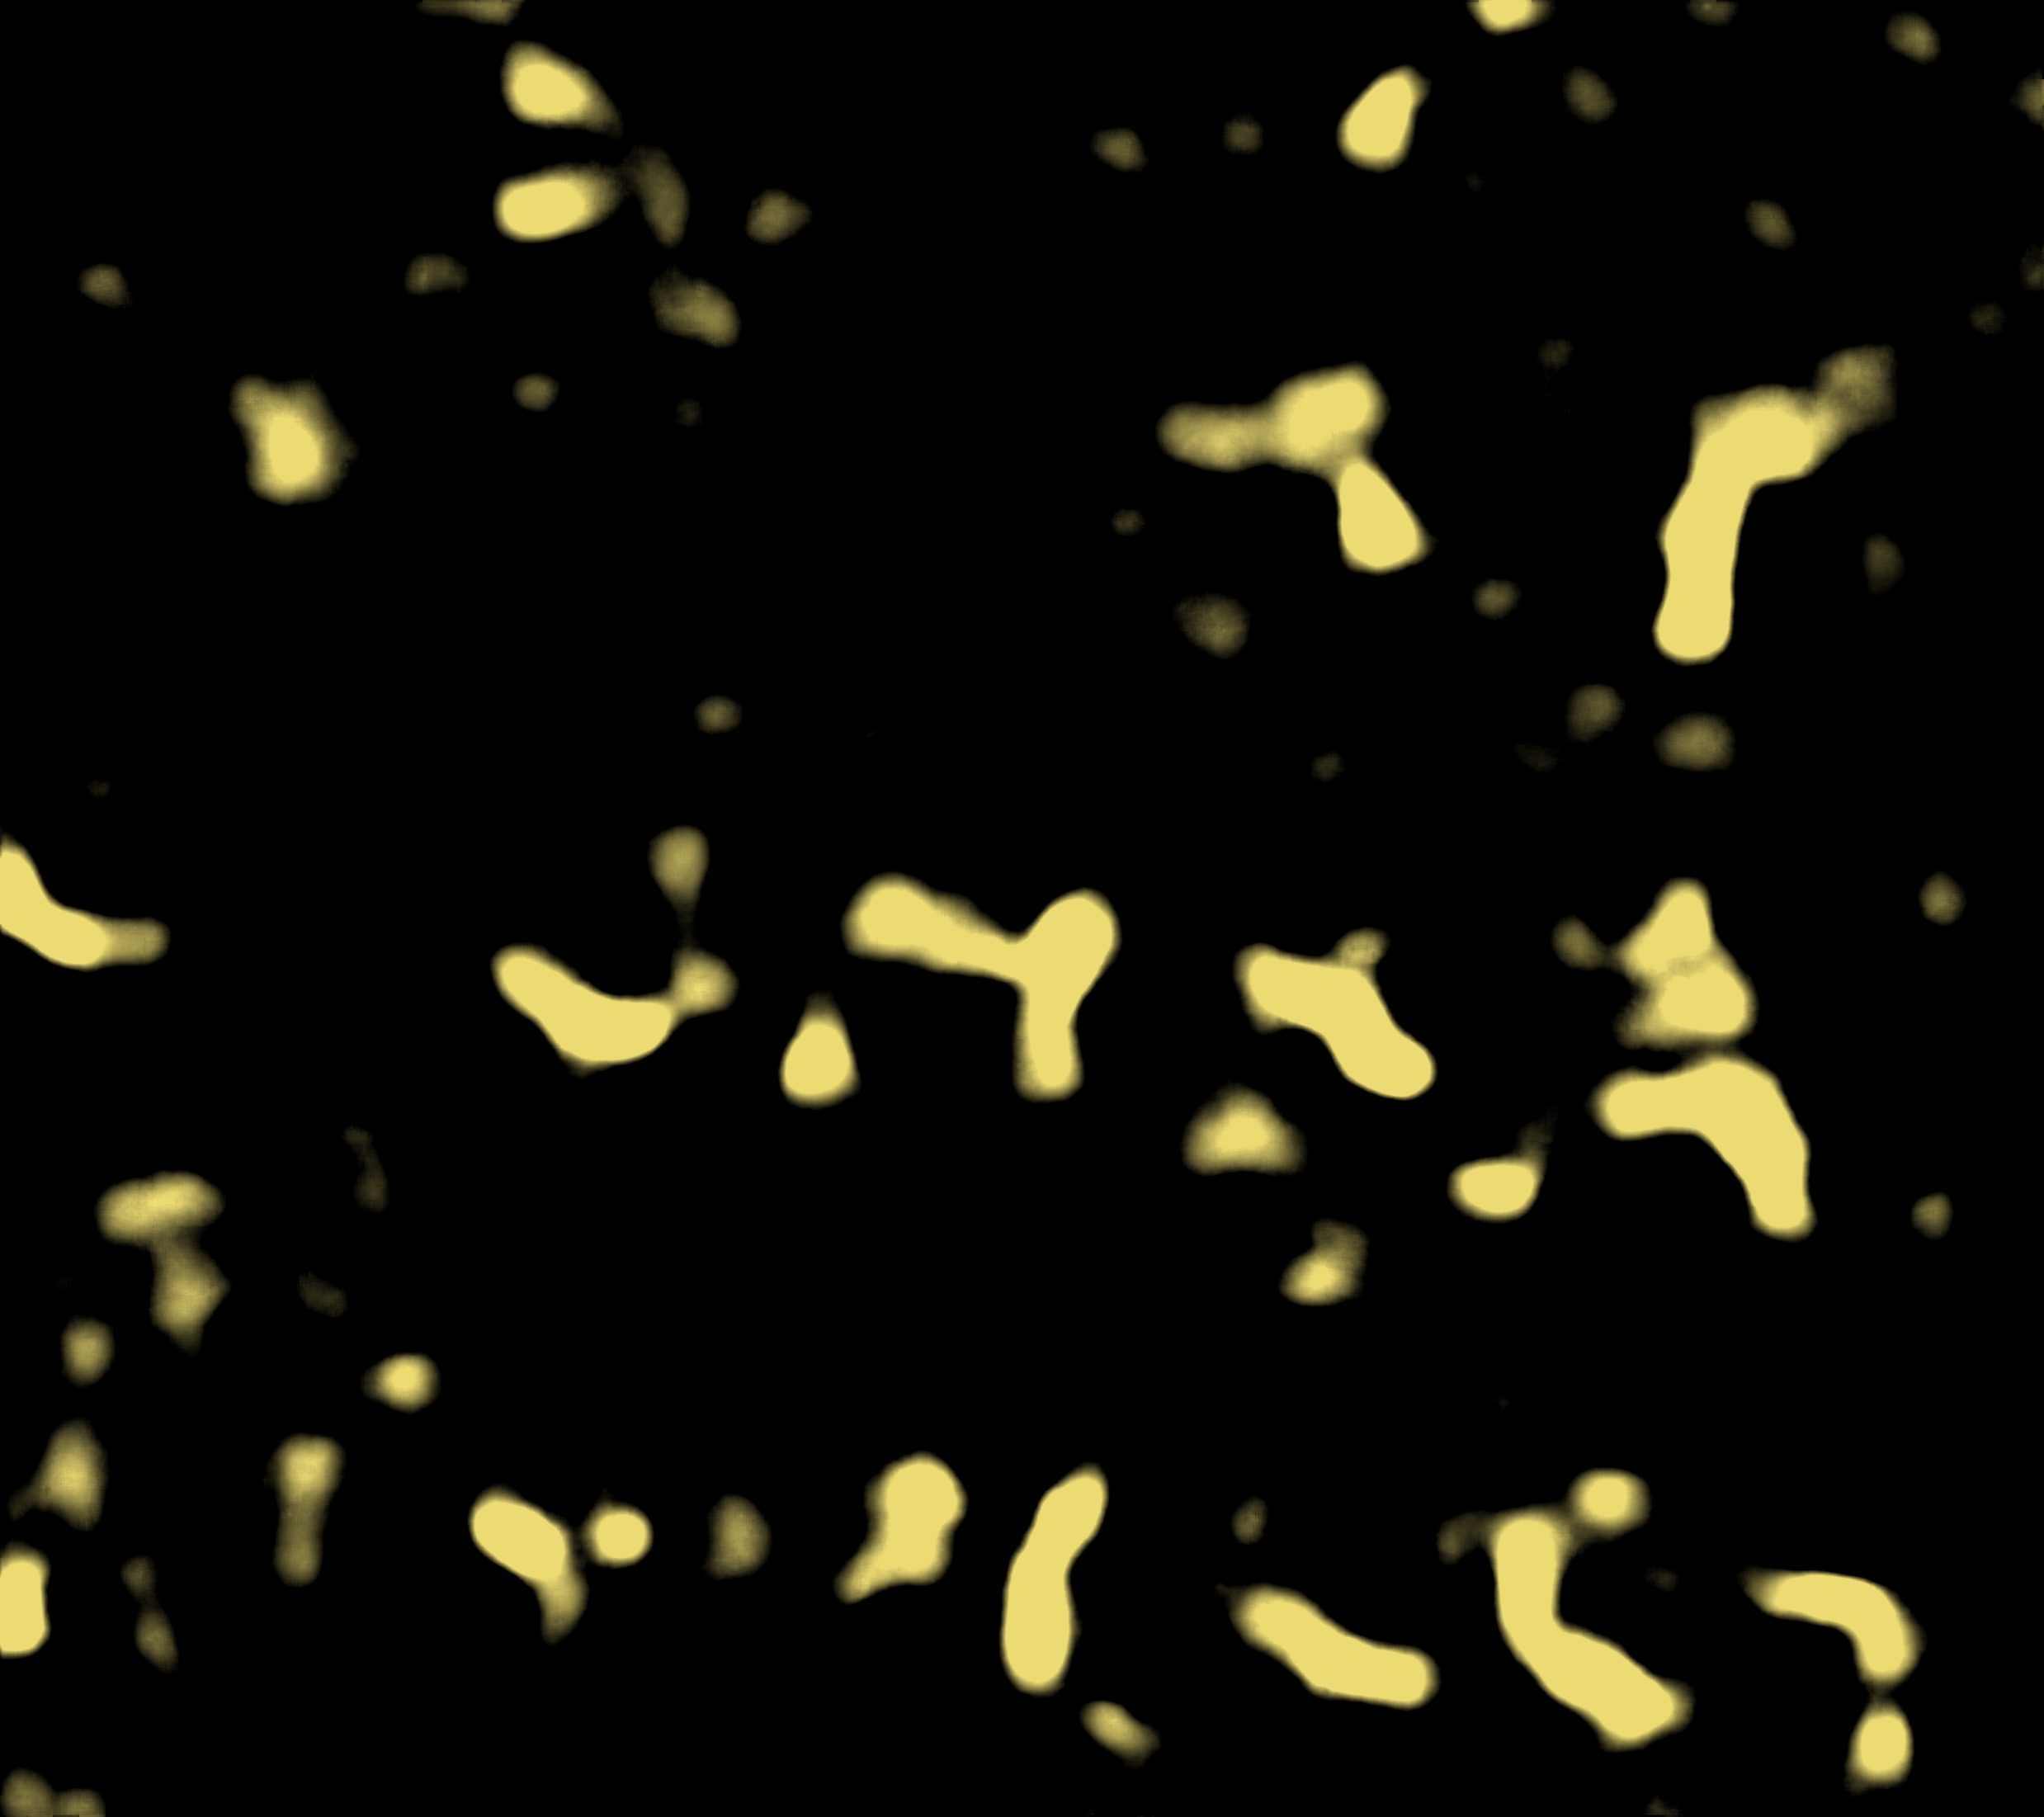
\includegraphics[width=122.48pt]{../figures/ag2/ag2_3_reader-v2.png}}\end{minipage}\hspace{2pt}\begin{minipage}[t]{122.48pt}\centering\href{https://raw.githubusercontent.com/evilaliv3/vesuvius-challenge-pipeline/main/results/db27c806-rectina/src/figures/ag2/ag2_5_rectina-m1.png}{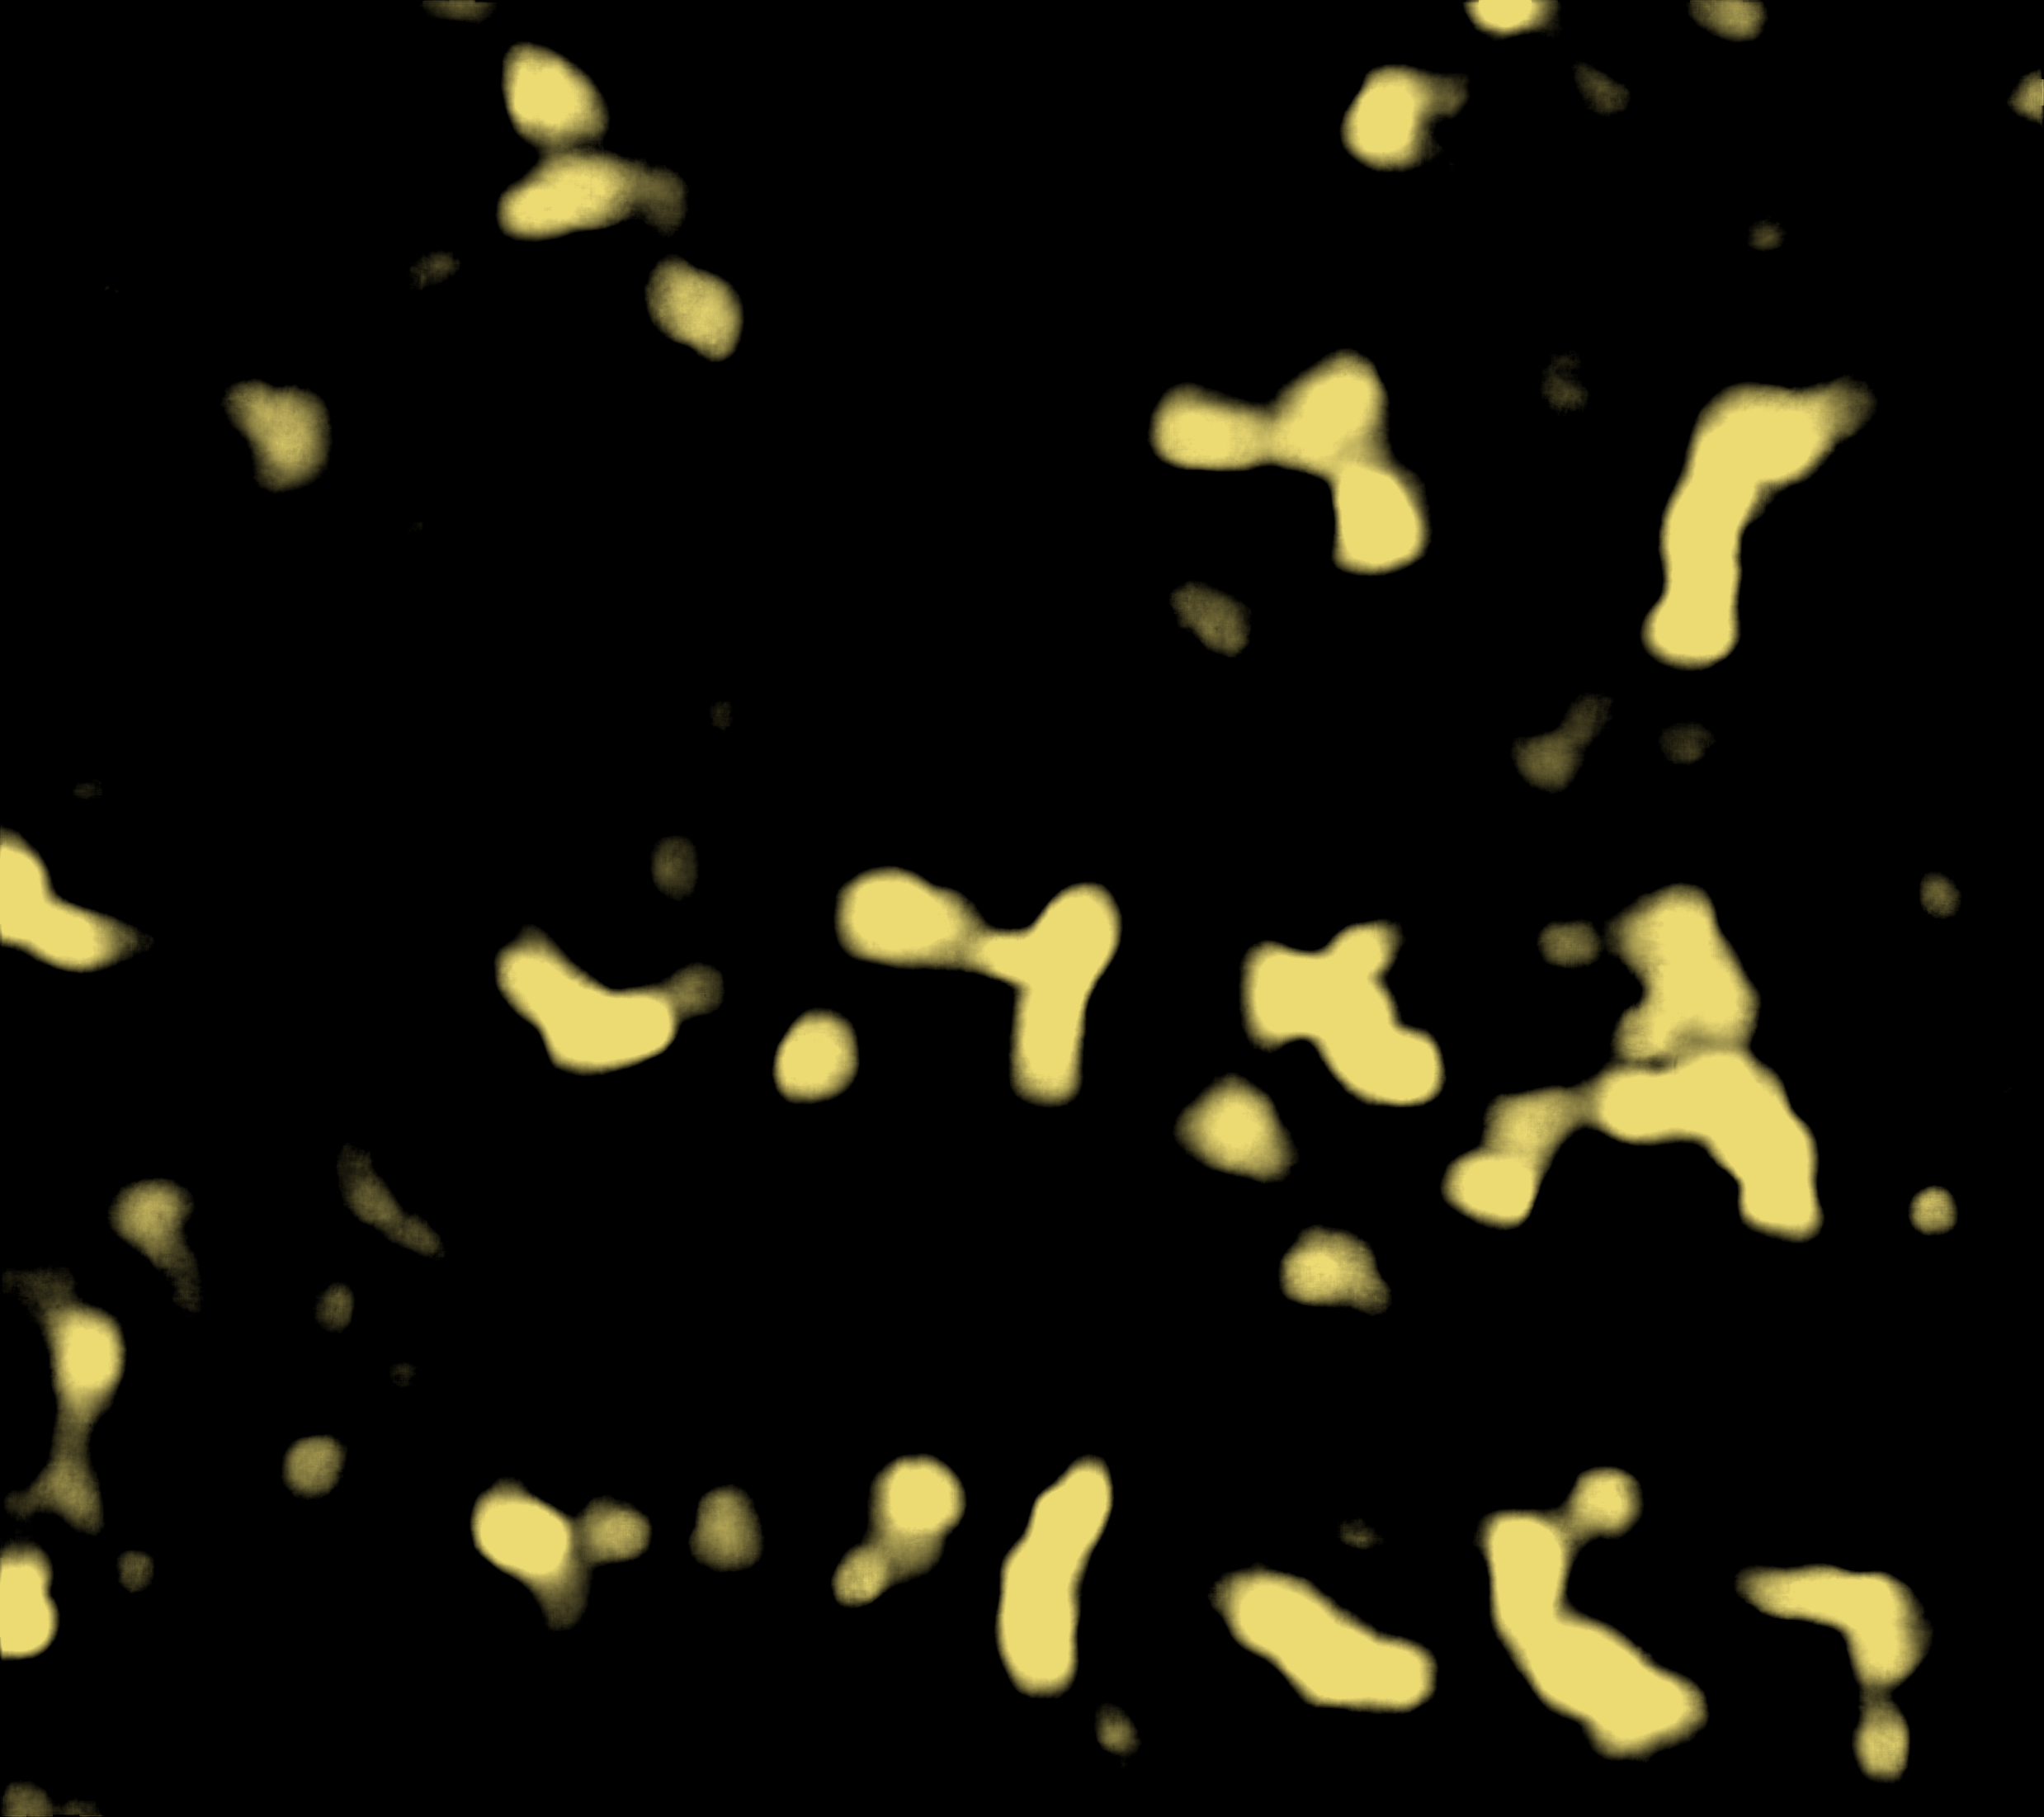
\includegraphics[width=122.48pt]{../figures/ag2/ag2_5_rectina-m1.png}}\end{minipage}}
\par\vspace{4pt}
\noindent\makebox[\columnwidth][c]{\begin{minipage}[t]{122.48pt}\centering\href{https://raw.githubusercontent.com/evilaliv3/vesuvius-challenge-pipeline/main/results/db27c806-rectina/src/figures/ag2/ag2_4_reader-v3.png}{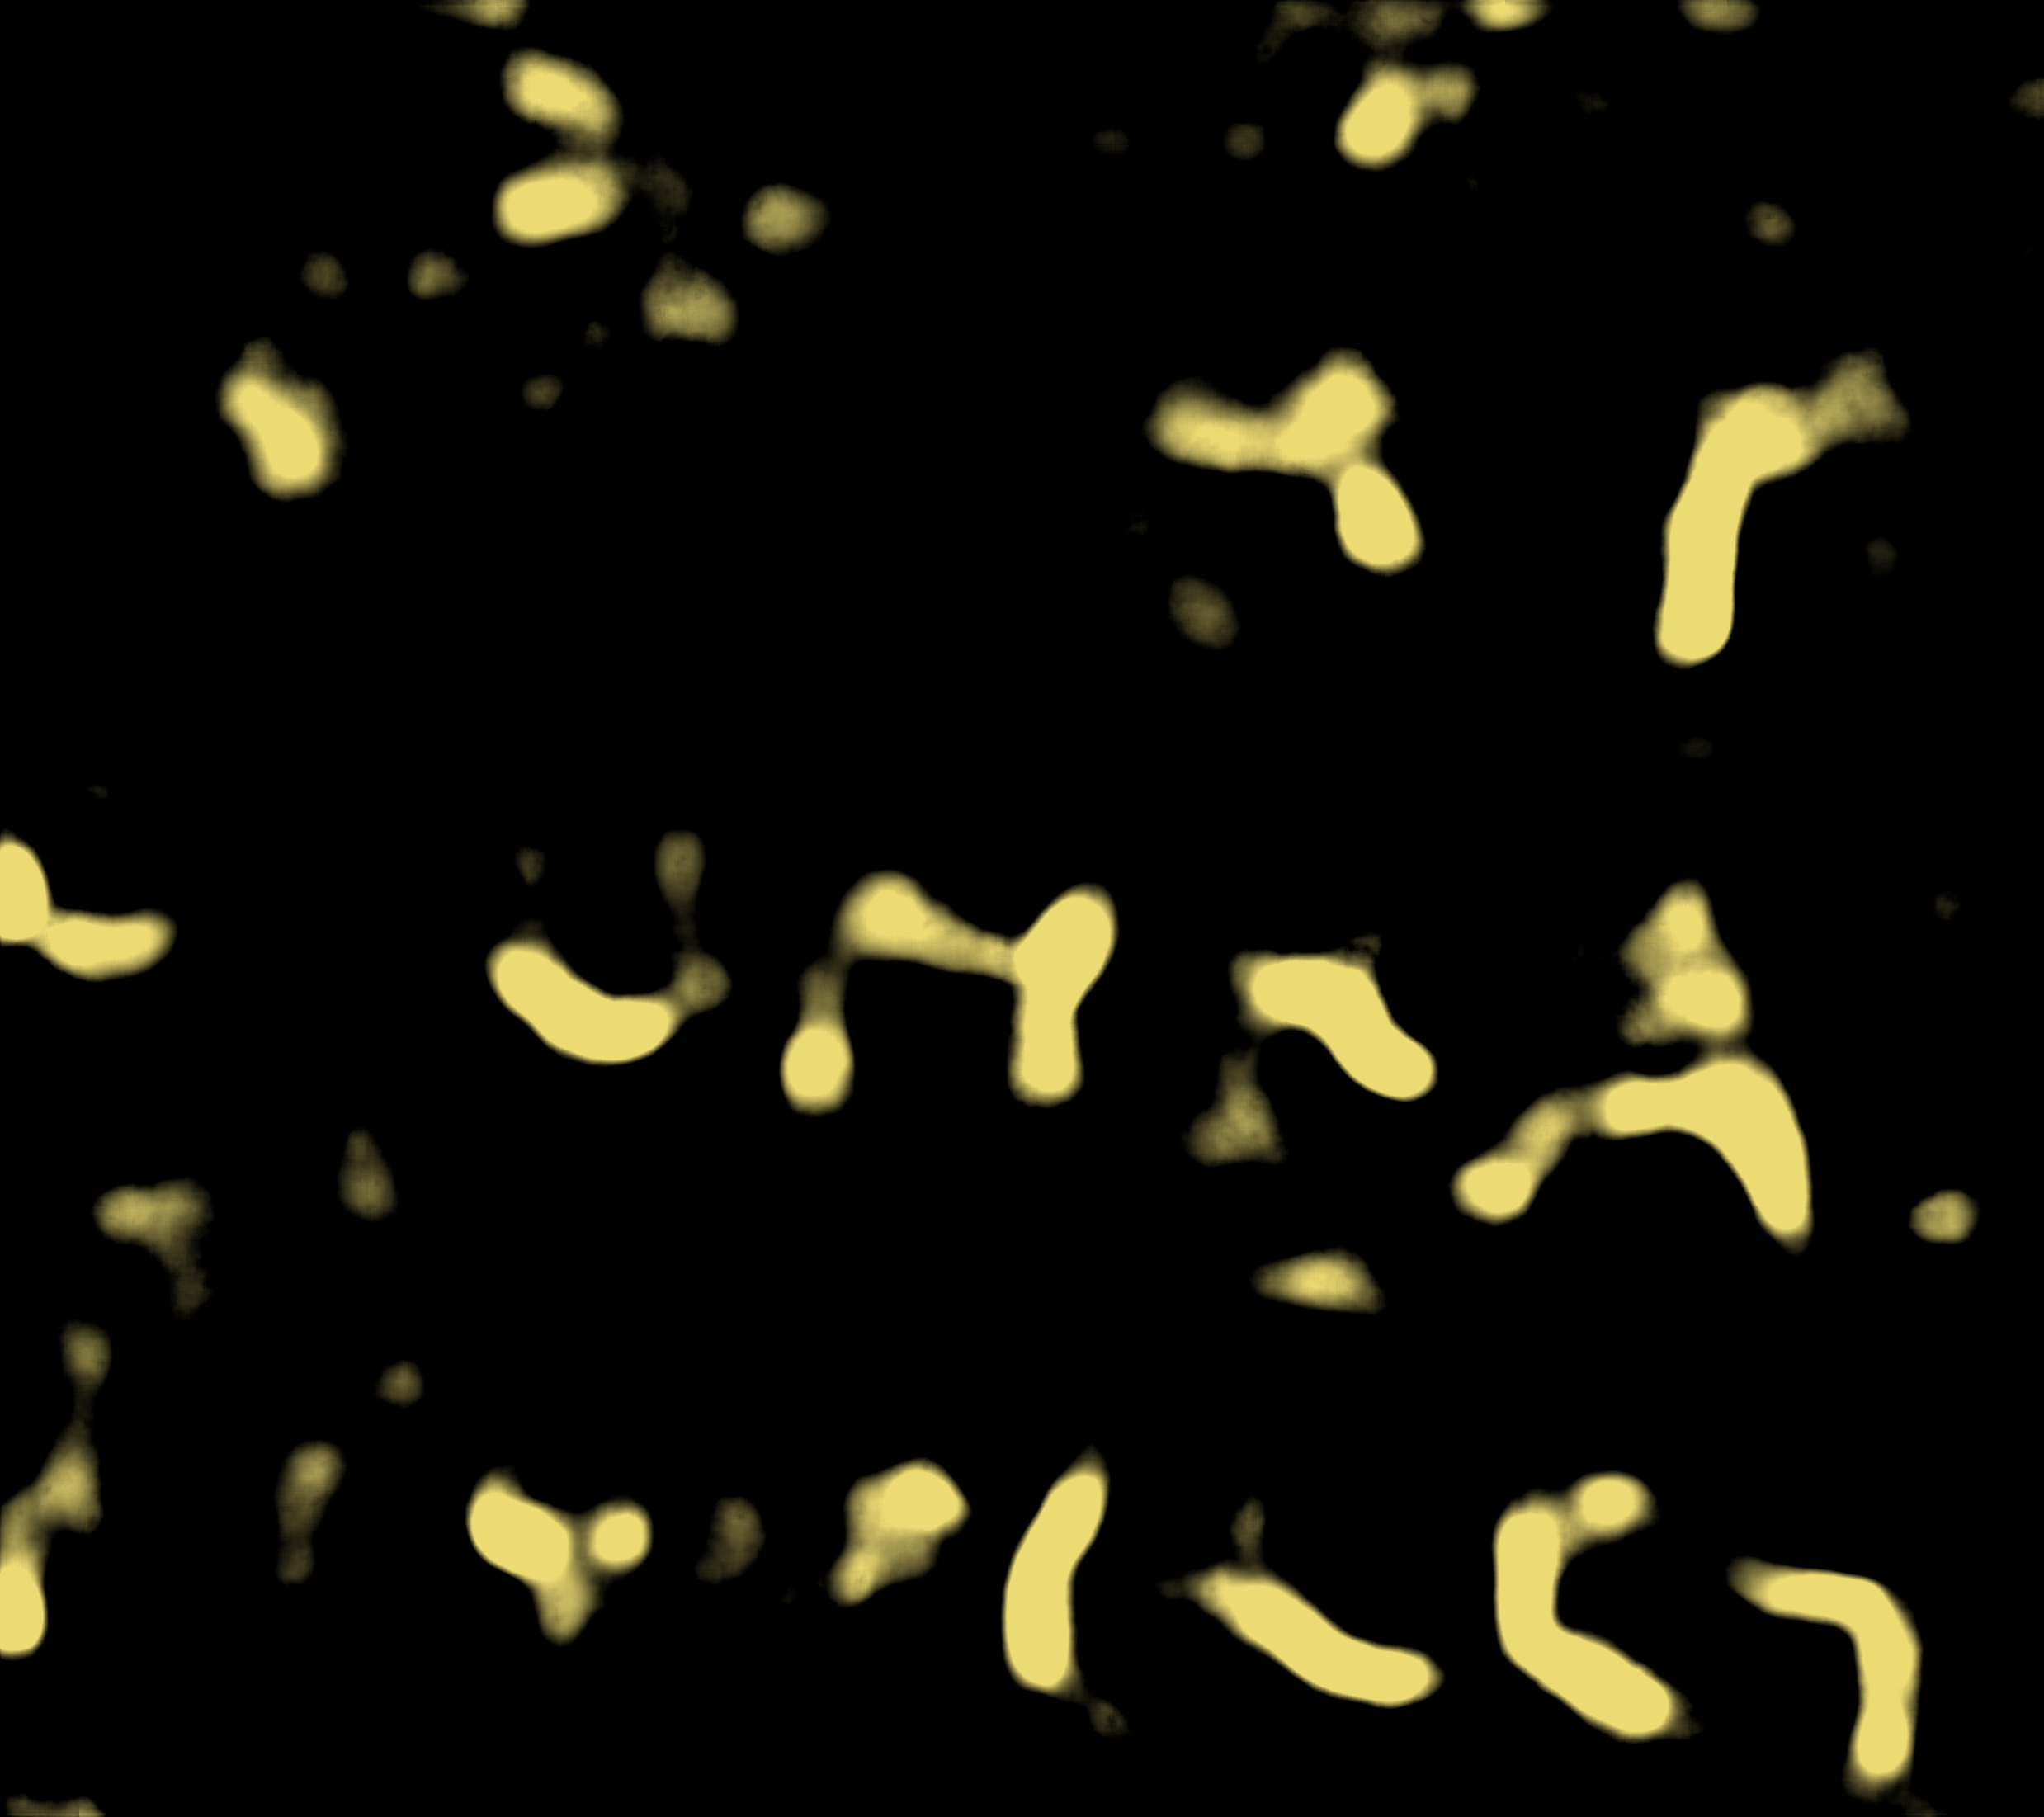
\includegraphics[width=122.48pt]{../figures/ag2/ag2_4_reader-v3.png}}\end{minipage}\hspace{2pt}\begin{minipage}[t]{122.48pt}\centering\href{https://raw.githubusercontent.com/evilaliv3/vesuvius-challenge-pipeline/main/results/db27c806-rectina/src/figures/ag2/ag2_6_rectina-m2.png}{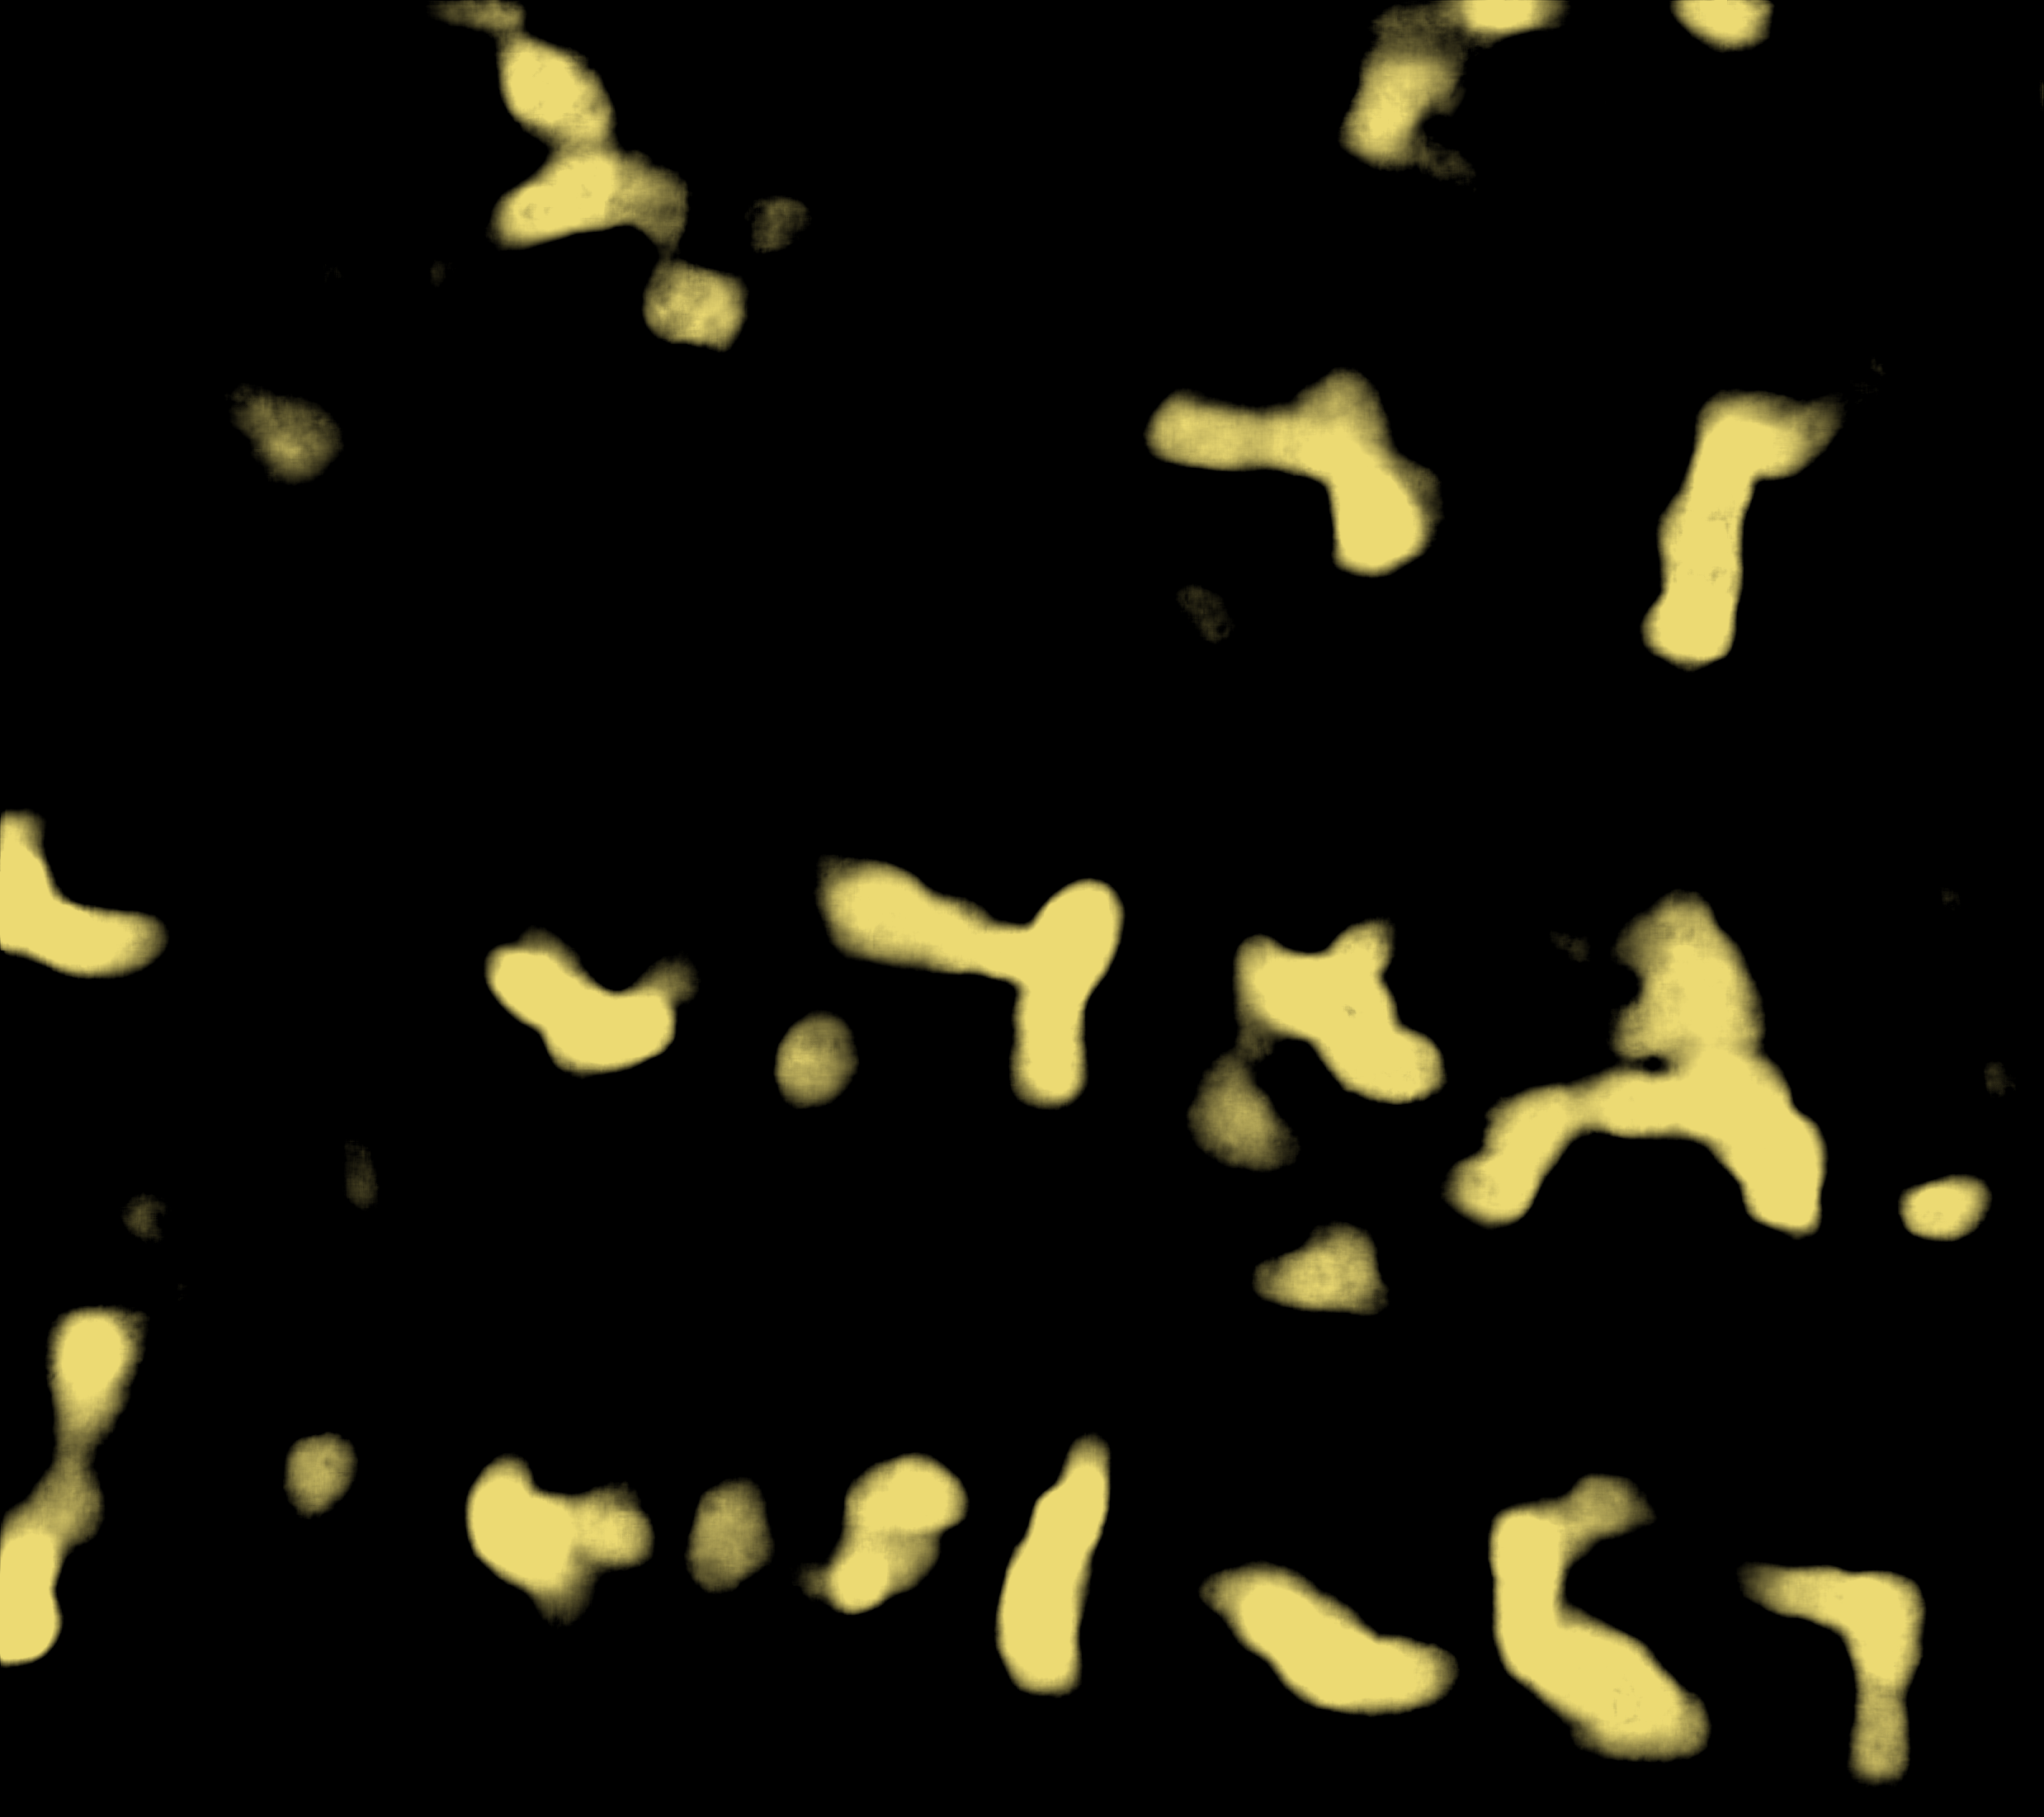
\includegraphics[width=122.48pt]{../figures/ag2/ag2_6_rectina-m2.png}}\end{minipage}}
\caption{Control unit 0841 ag2, three rows of two panels. Row 1: left, Texture; right, Labels. Row 2: left, Reader v2; right, Rectina m1 (display windows: Reader v2 0.404870 to 0.589240 (ramp); Rectina m1 0.560881 to 0.723274 (ramp)). Row 3: left, Reader v3; right, Rectina m2 (display windows: Reader v3 0.431564 to 0.660926 (ramp); Rectina m2 0.615411 to 0.768217 (ramp)). Each map is stretched between its own percentiles. Reader and model stand side by side in the rows 2 and 3.}
\end{figure}

\begin{figure}[!tbp]
\centering
\noindent\makebox[\columnwidth][c]{\begin{minipage}[t]{122.48pt}\centering\href{https://raw.githubusercontent.com/evilaliv3/vesuvius-challenge-pipeline/main/results/db27c806-rectina/src/figures/w00/w00_1_texture.png}{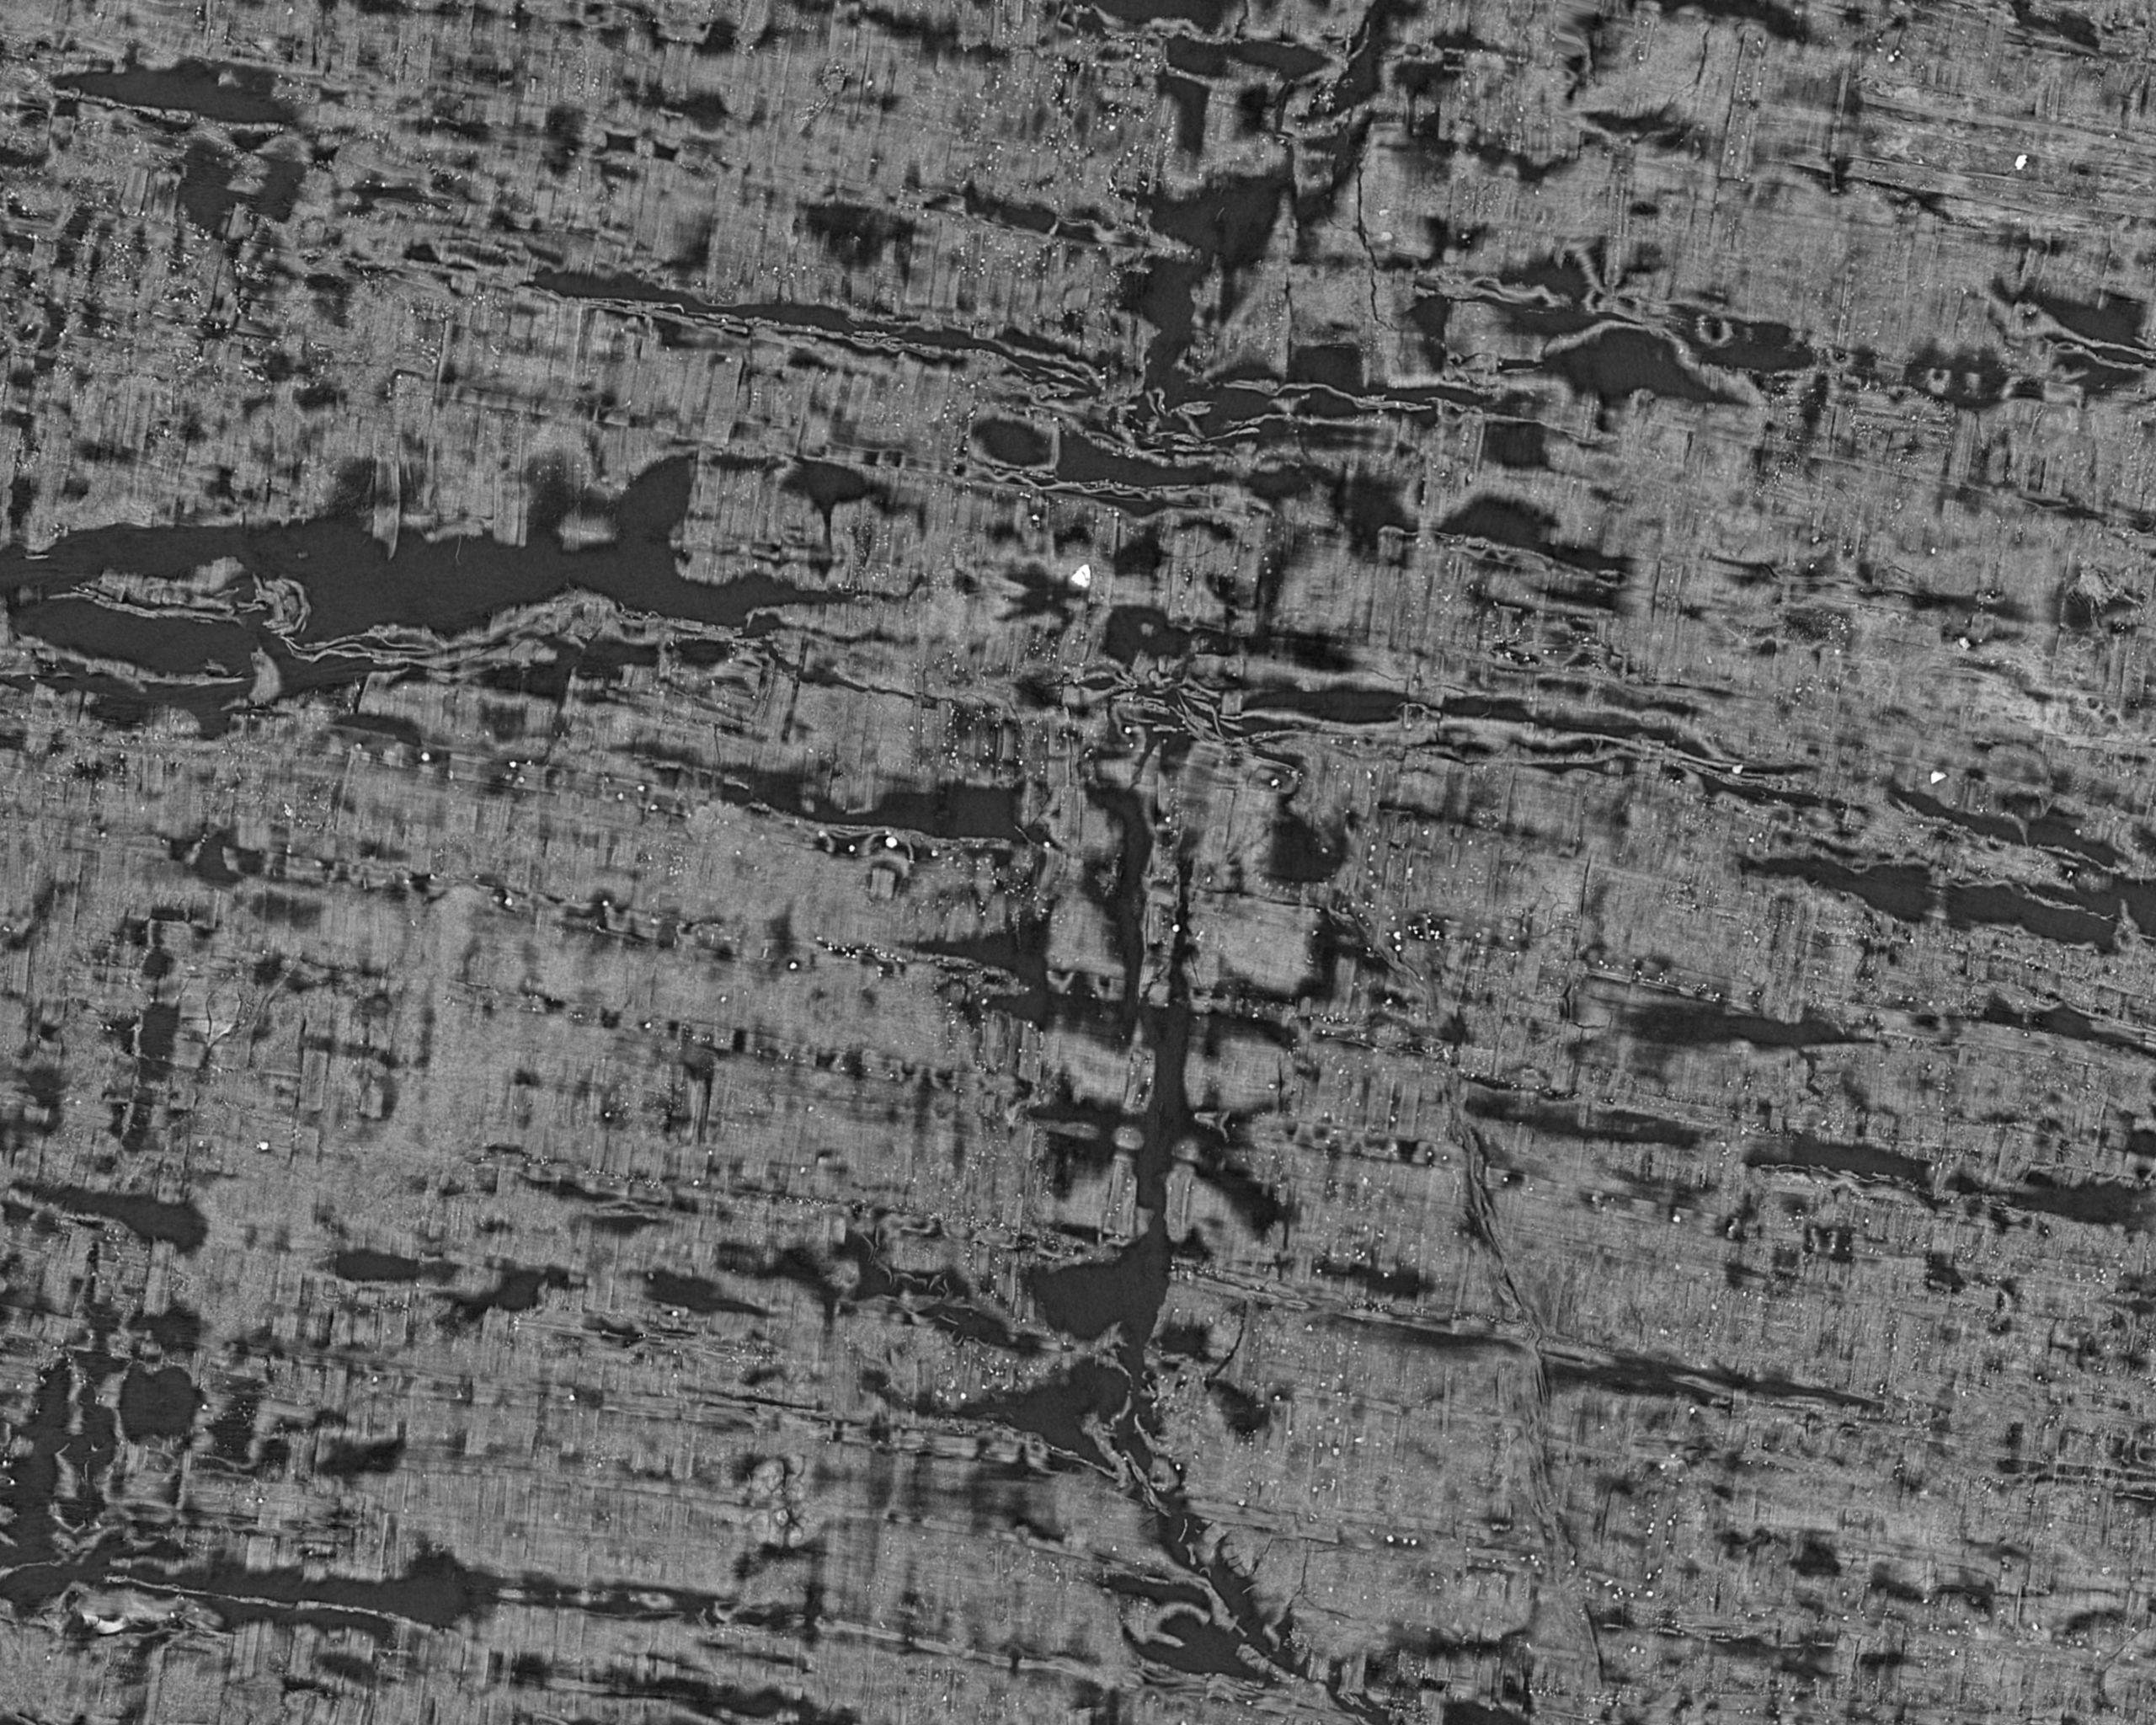
\includegraphics[width=122.48pt]{../figures/w00/w00_1_texture.png}}\end{minipage}\hspace{2pt}\begin{minipage}[t]{122.48pt}\centering\href{https://raw.githubusercontent.com/evilaliv3/vesuvius-challenge-pipeline/main/results/db27c806-rectina/src/figures/w00/w00_2_labels.png}{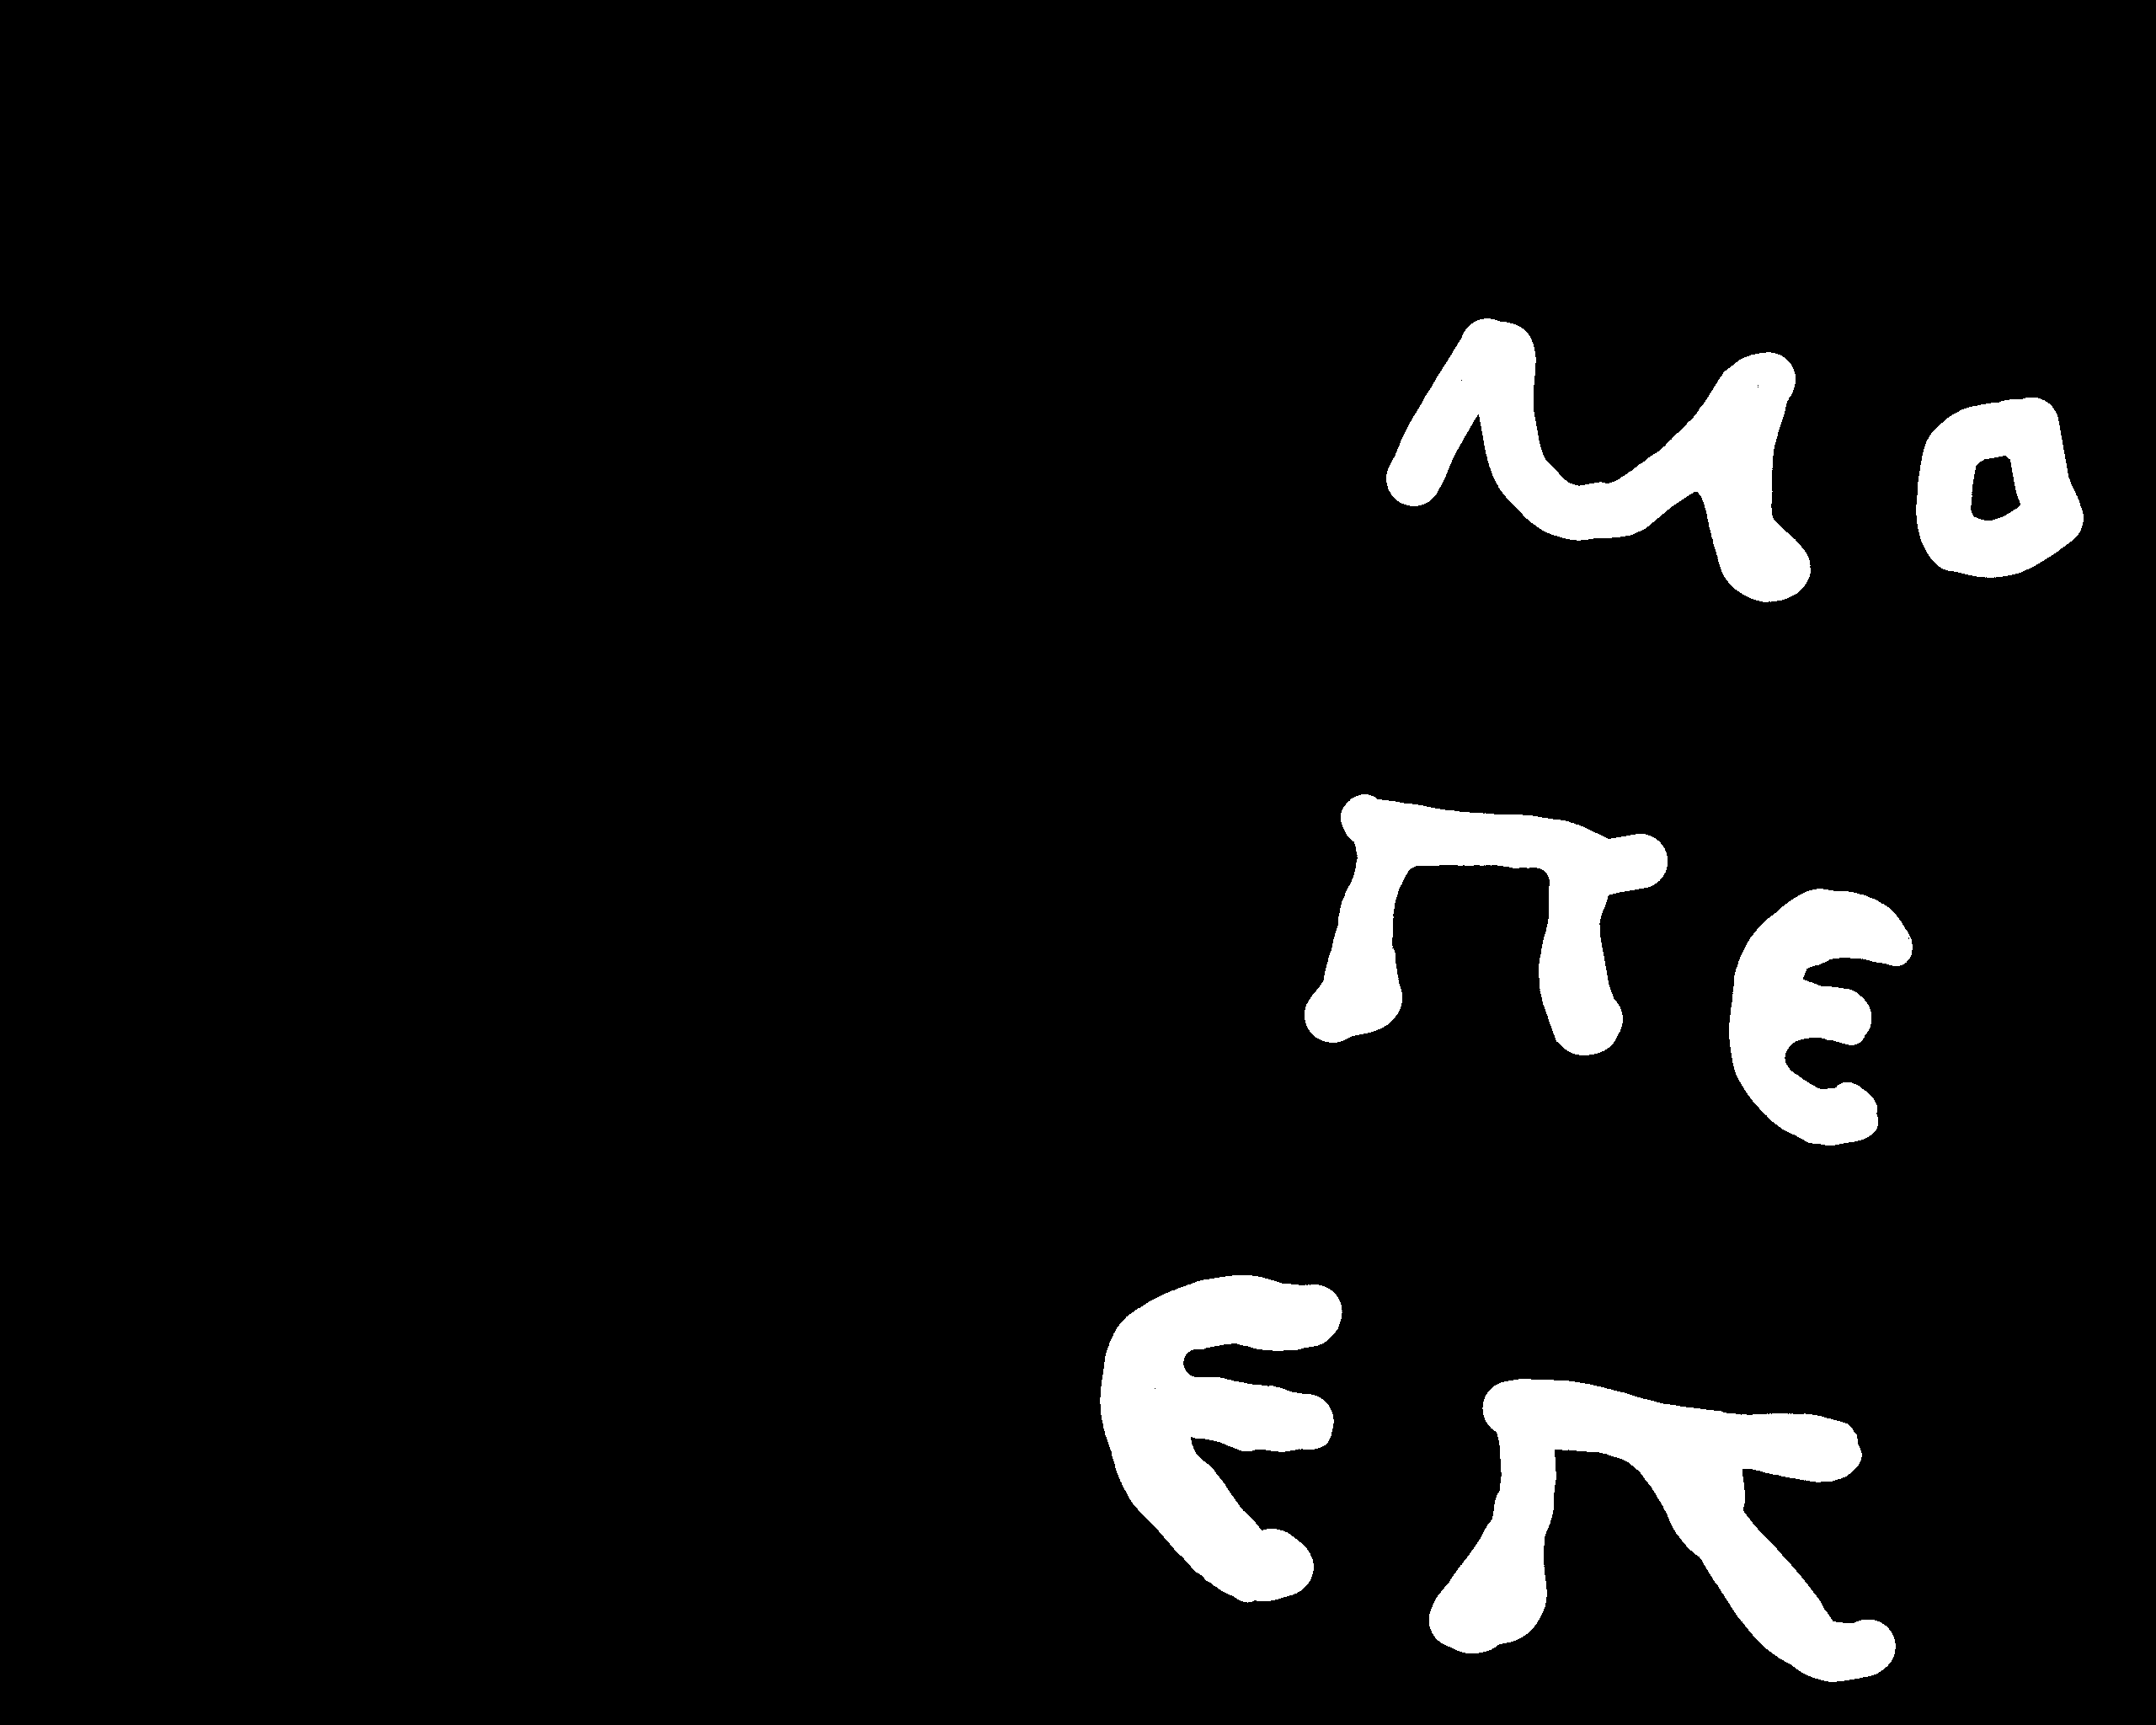
\includegraphics[width=122.48pt]{../figures/w00/w00_2_labels.png}}\end{minipage}}
\par\vspace{4pt}
\noindent\makebox[\columnwidth][c]{\begin{minipage}[t]{122.48pt}\centering\href{https://raw.githubusercontent.com/evilaliv3/vesuvius-challenge-pipeline/main/results/db27c806-rectina/src/figures/w00/w00_3_reader-v2.png}{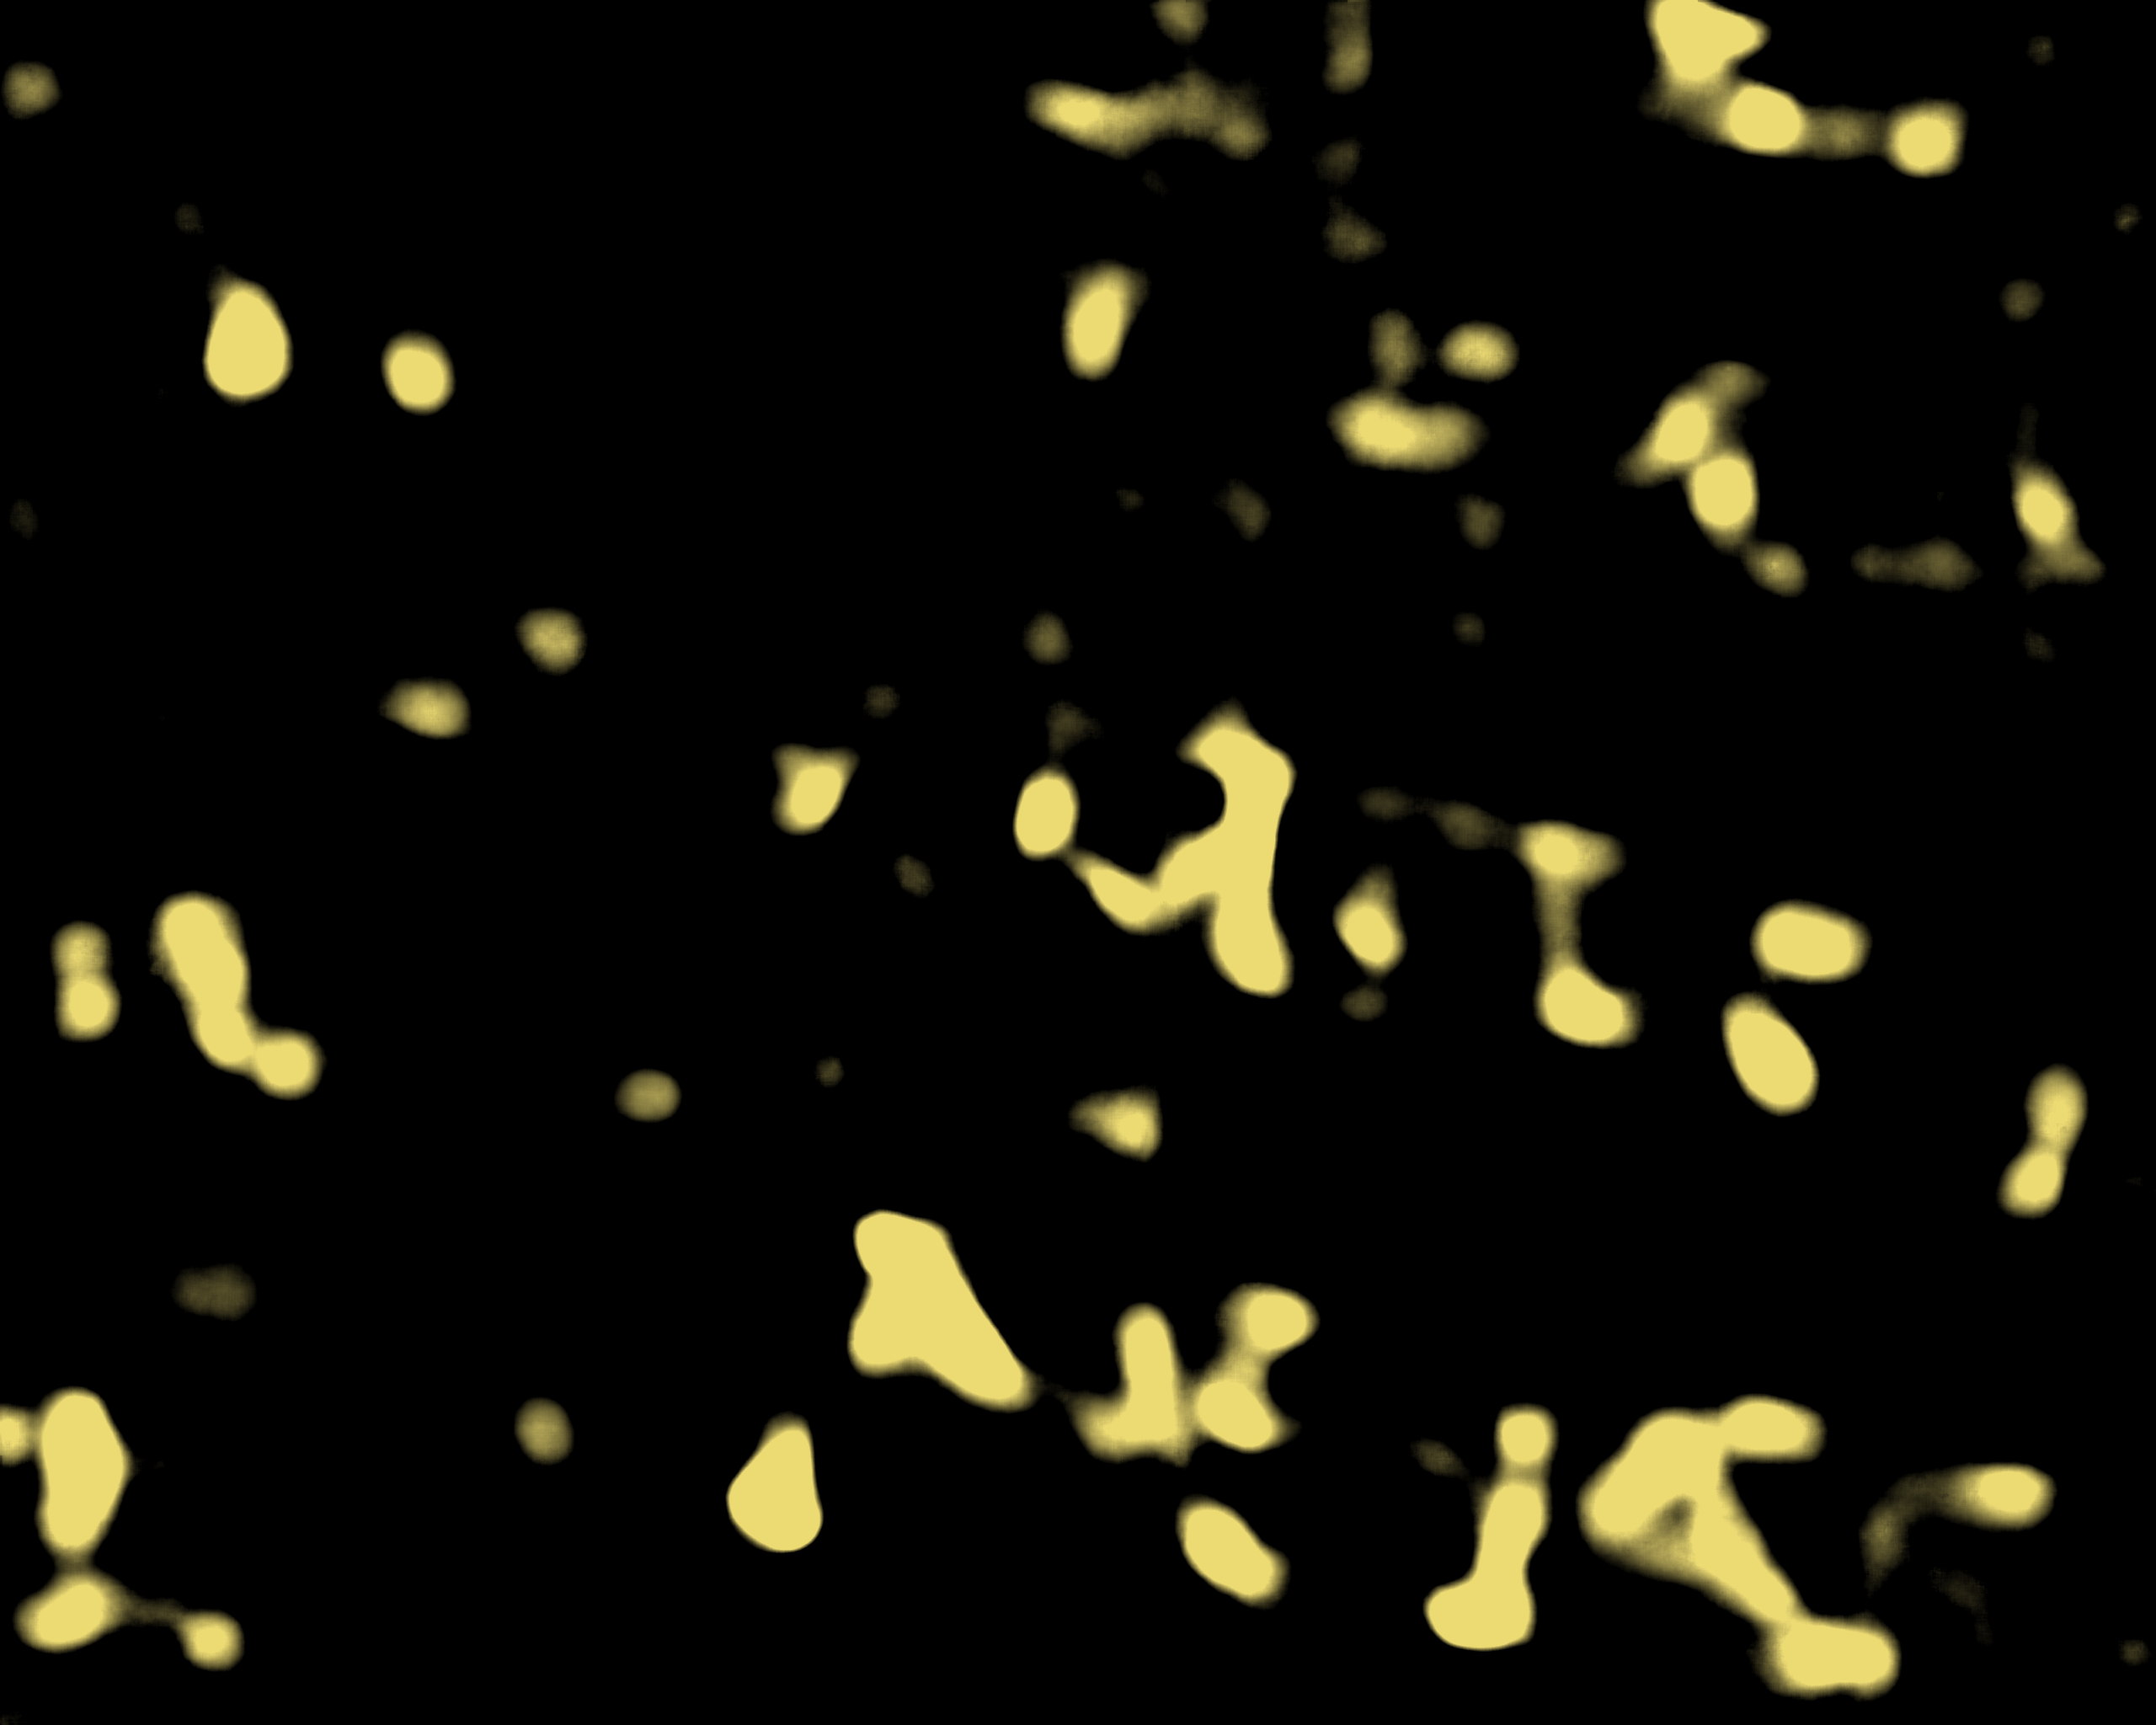
\includegraphics[width=122.48pt]{../figures/w00/w00_3_reader-v2.png}}\end{minipage}\hspace{2pt}\begin{minipage}[t]{122.48pt}\centering\href{https://raw.githubusercontent.com/evilaliv3/vesuvius-challenge-pipeline/main/results/db27c806-rectina/src/figures/w00/w00_5_rectina-m1.png}{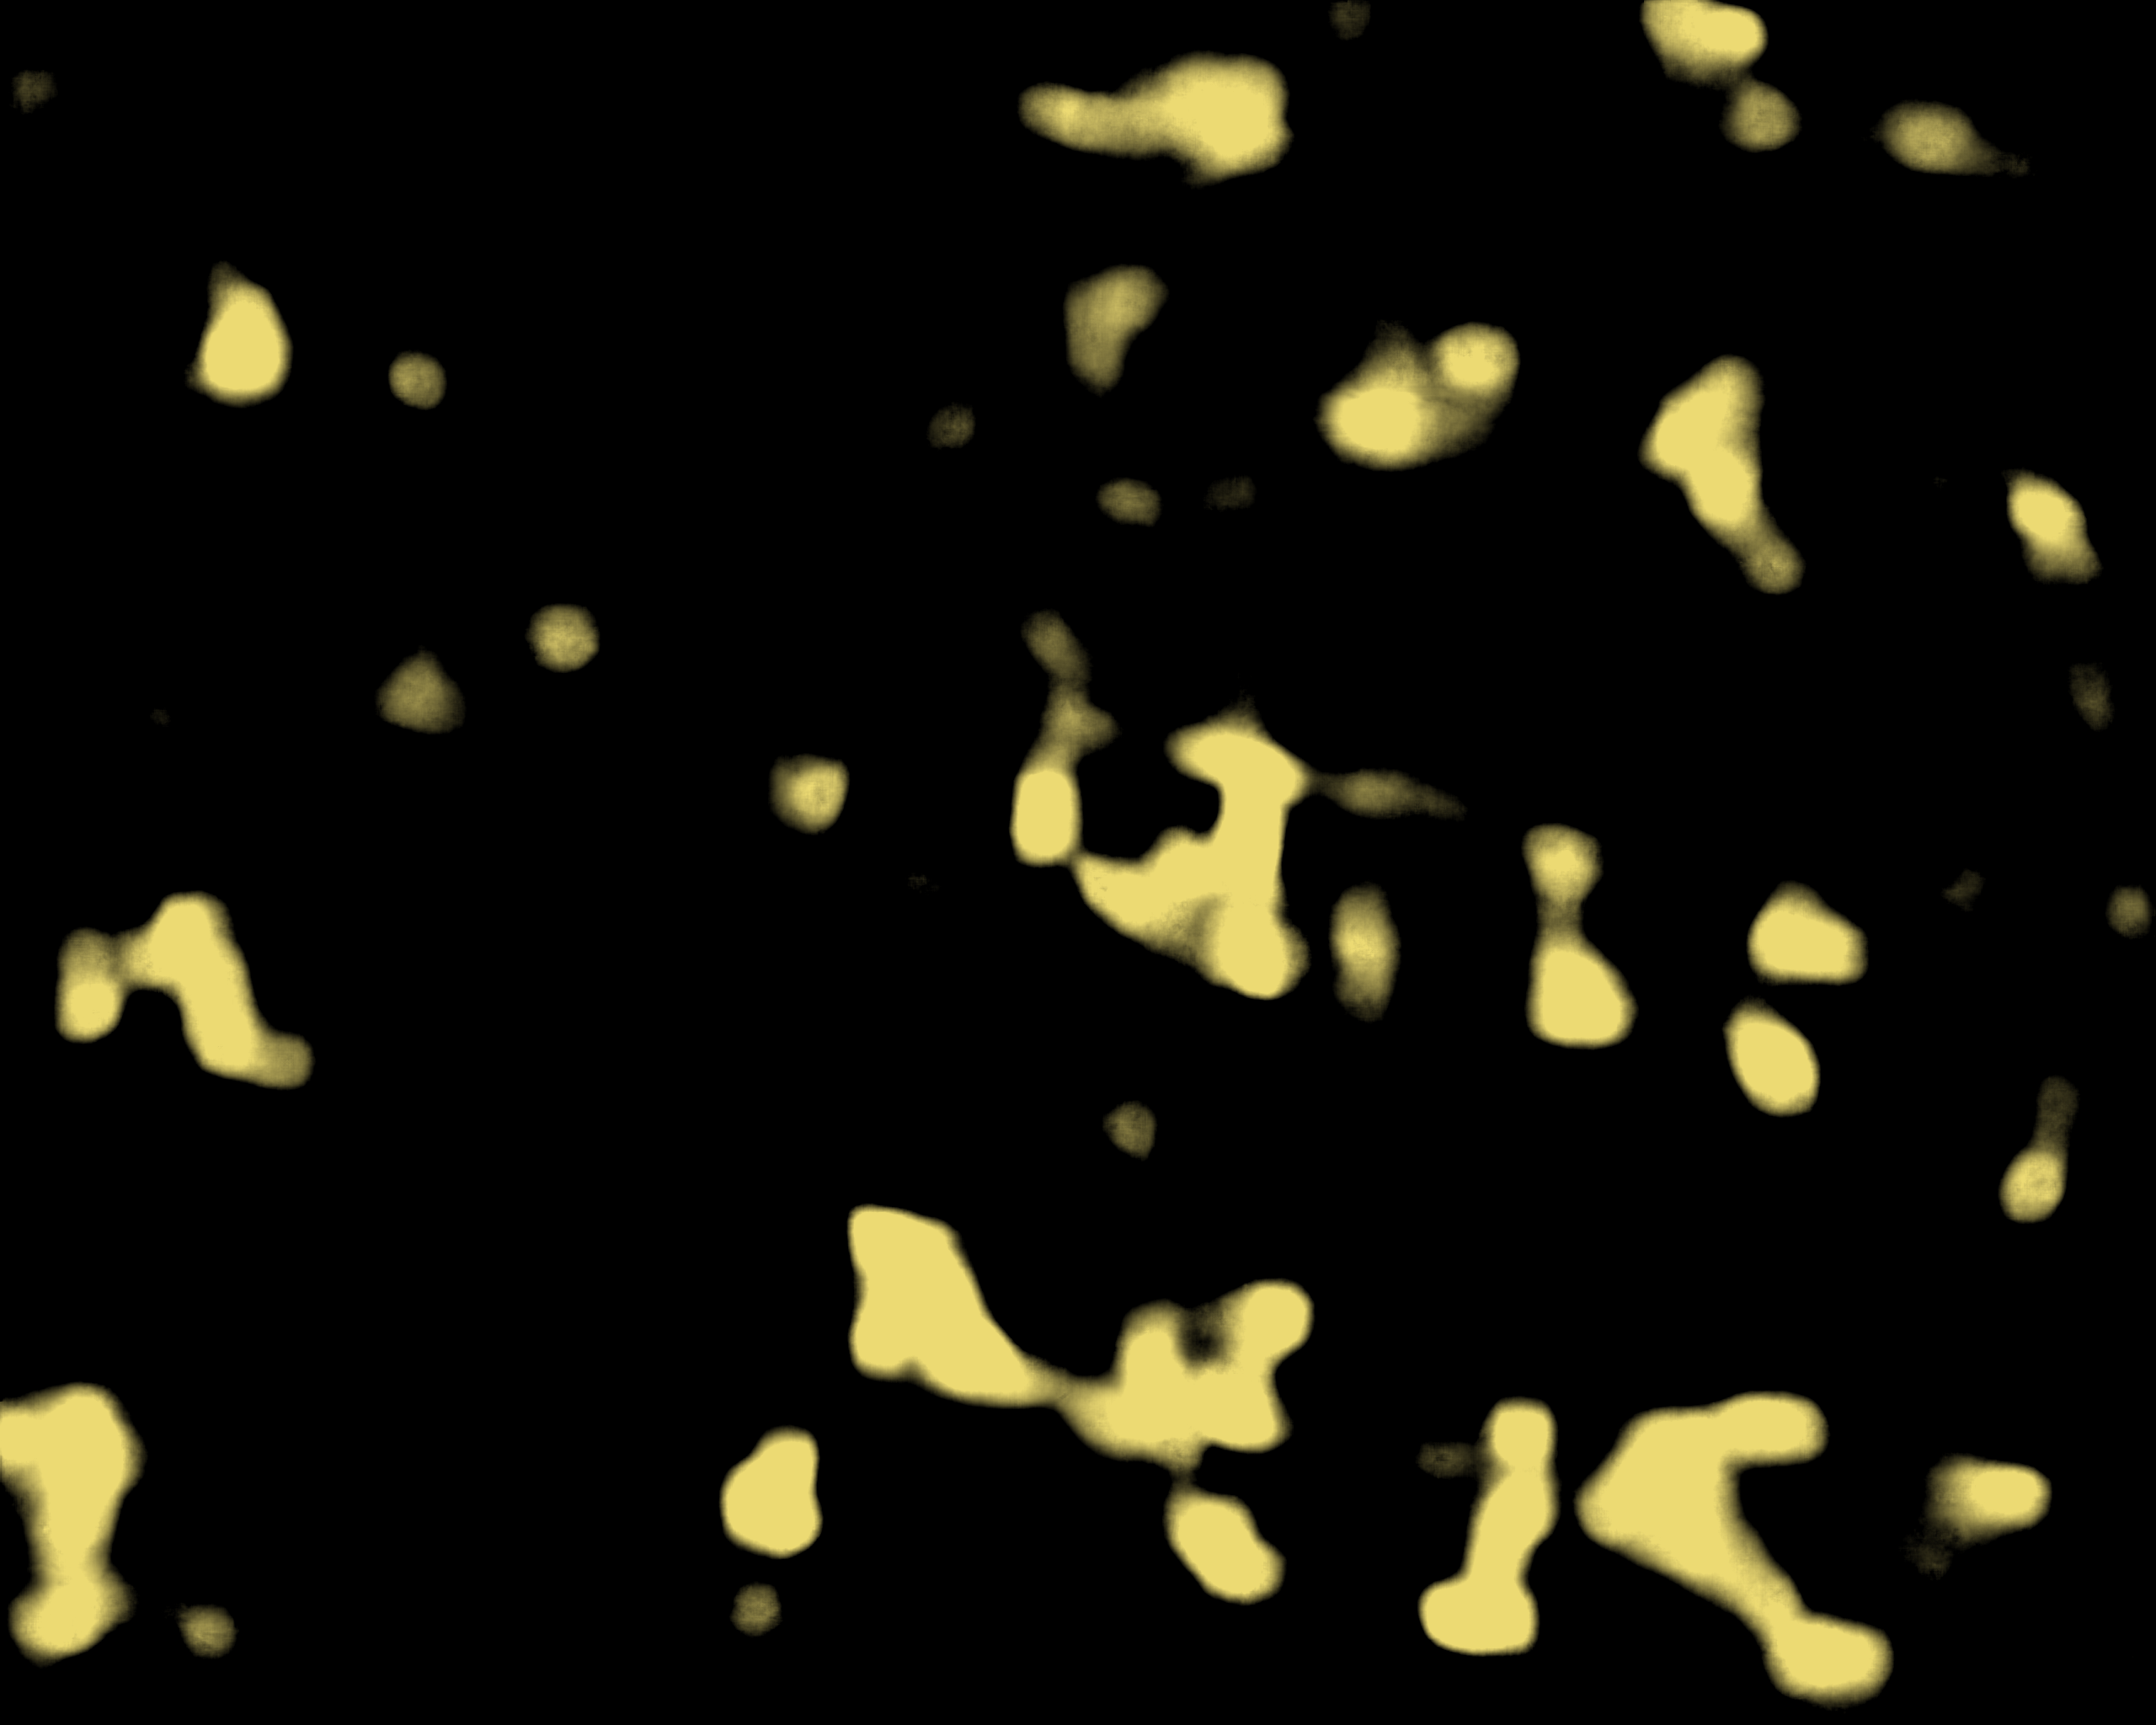
\includegraphics[width=122.48pt]{../figures/w00/w00_5_rectina-m1.png}}\end{minipage}}
\par\vspace{4pt}
\noindent\makebox[\columnwidth][c]{\begin{minipage}[t]{122.48pt}\centering\href{https://raw.githubusercontent.com/evilaliv3/vesuvius-challenge-pipeline/main/results/db27c806-rectina/src/figures/w00/w00_4_reader-v3.png}{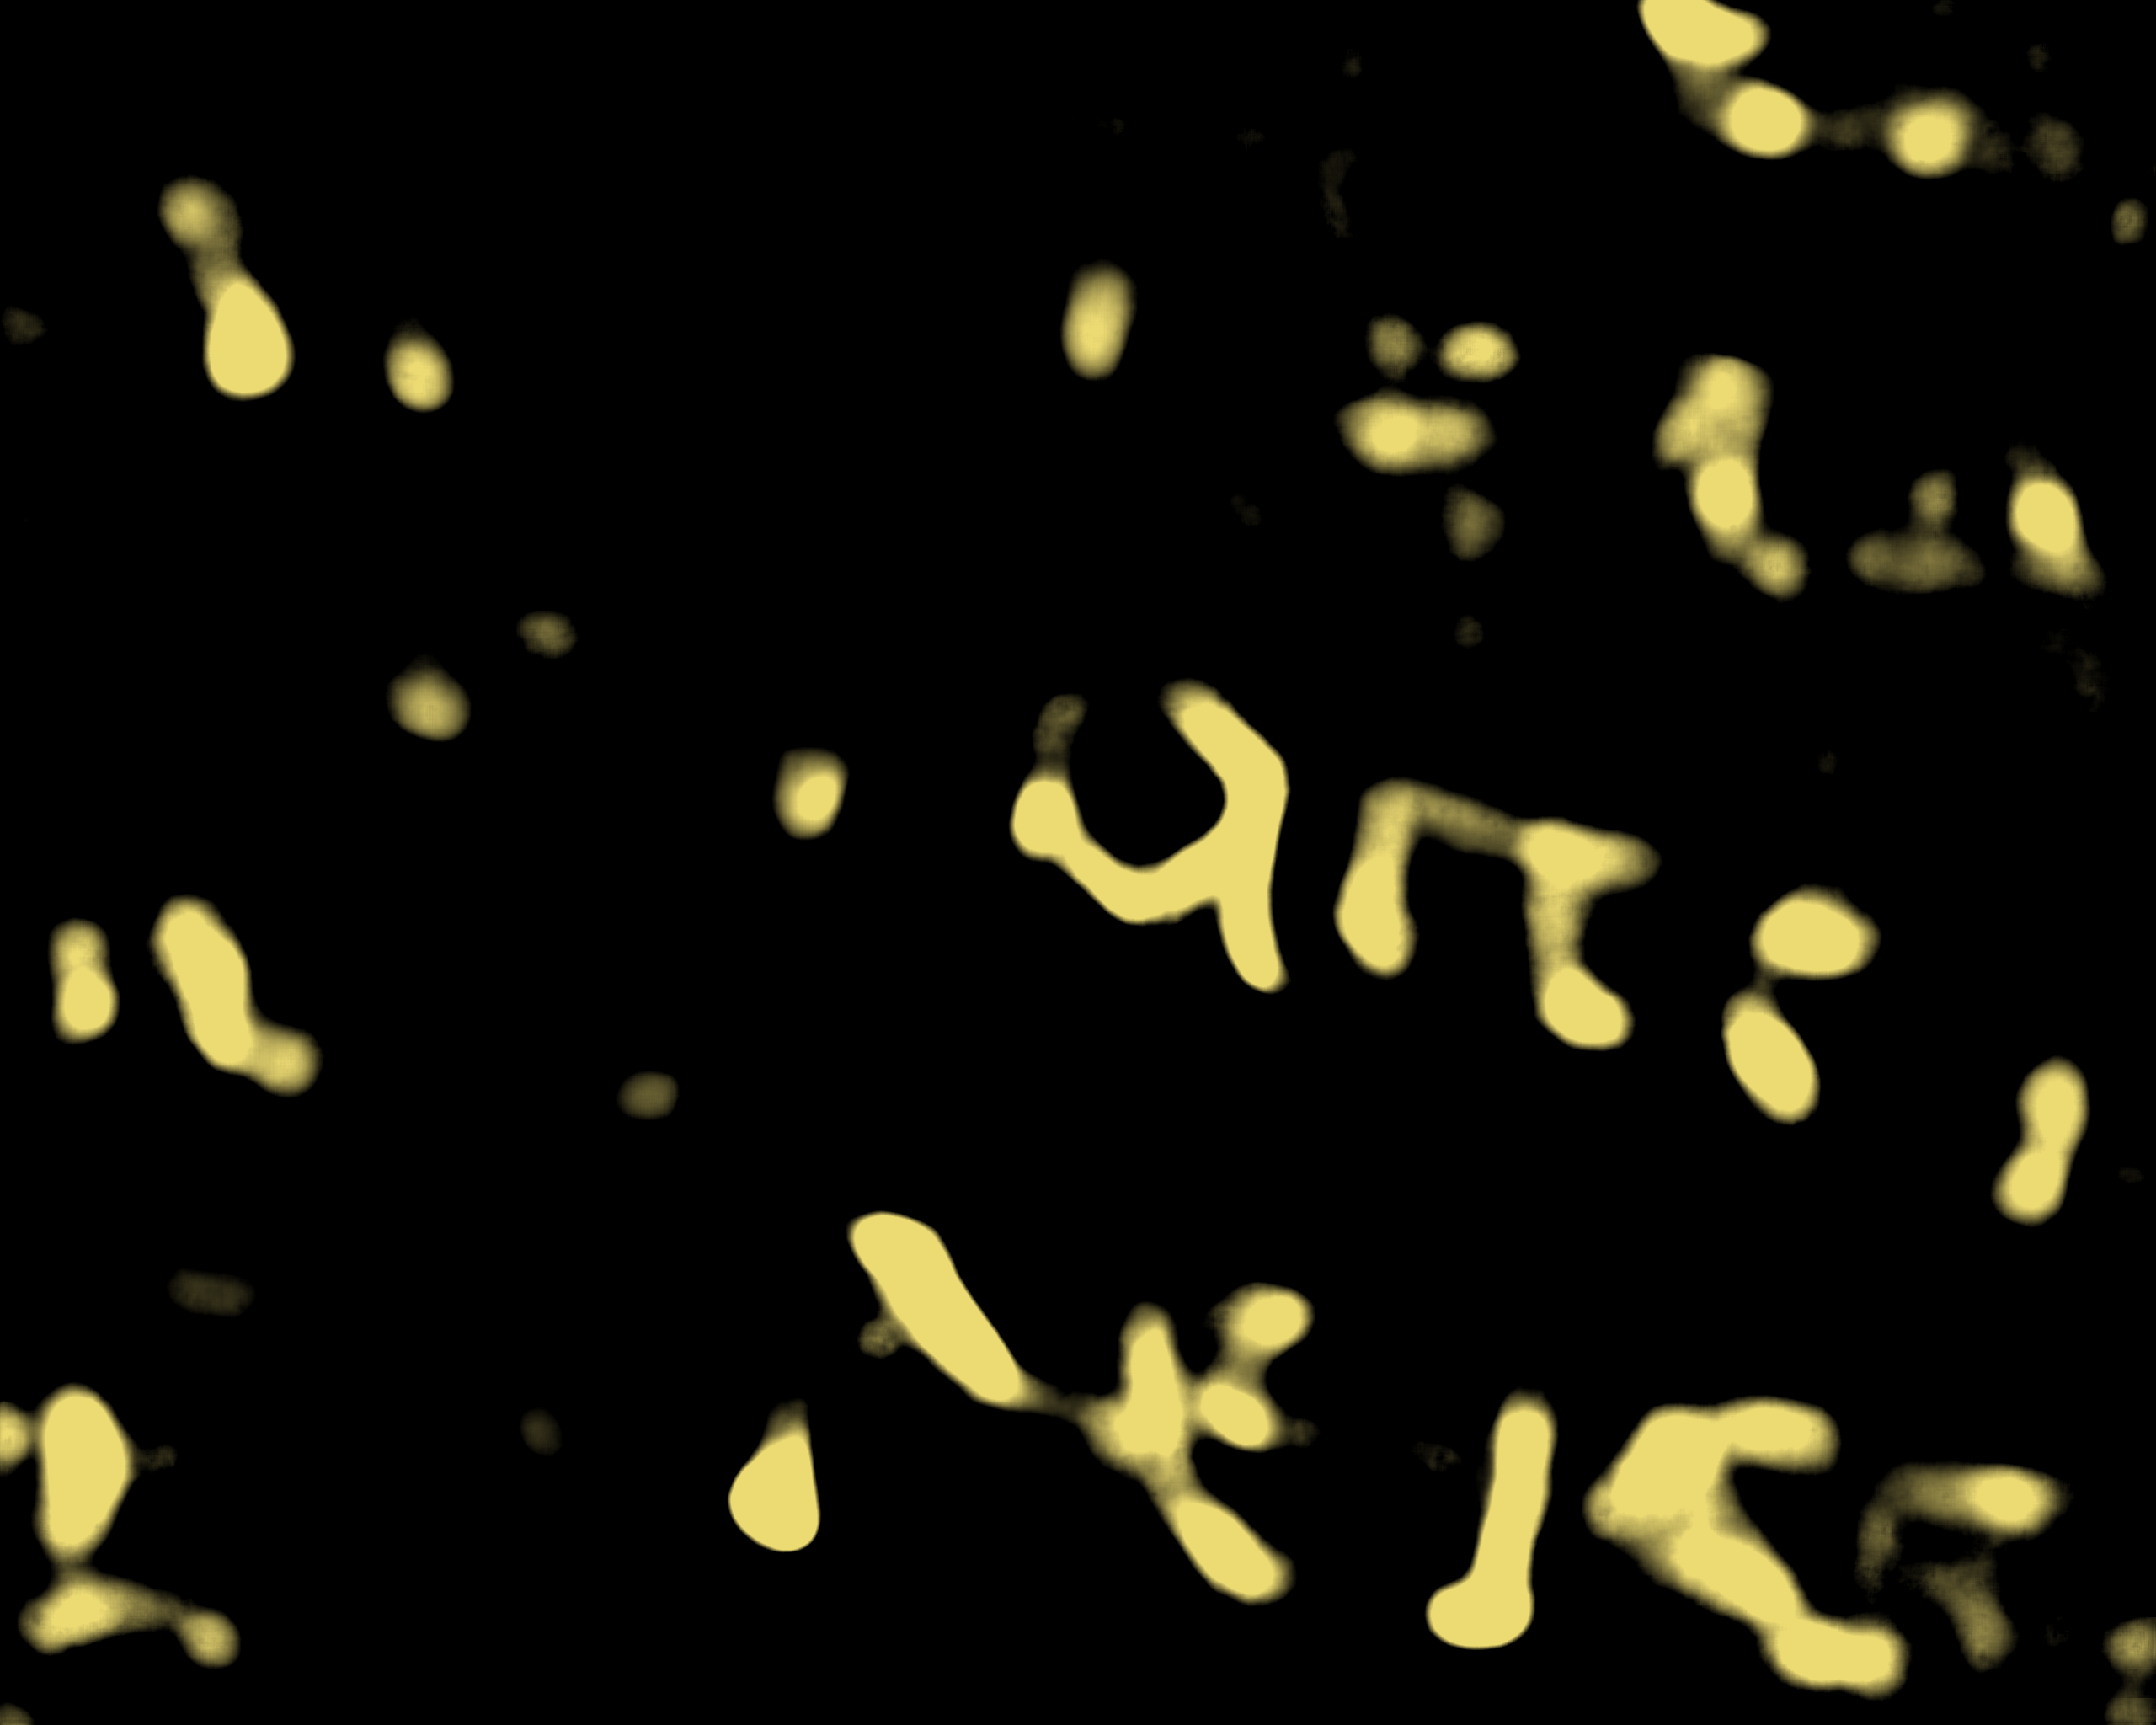
\includegraphics[width=122.48pt]{../figures/w00/w00_4_reader-v3.png}}\end{minipage}\hspace{2pt}\begin{minipage}[t]{122.48pt}\centering\href{https://raw.githubusercontent.com/evilaliv3/vesuvius-challenge-pipeline/main/results/db27c806-rectina/src/figures/w00/w00_6_rectina-m2.png}{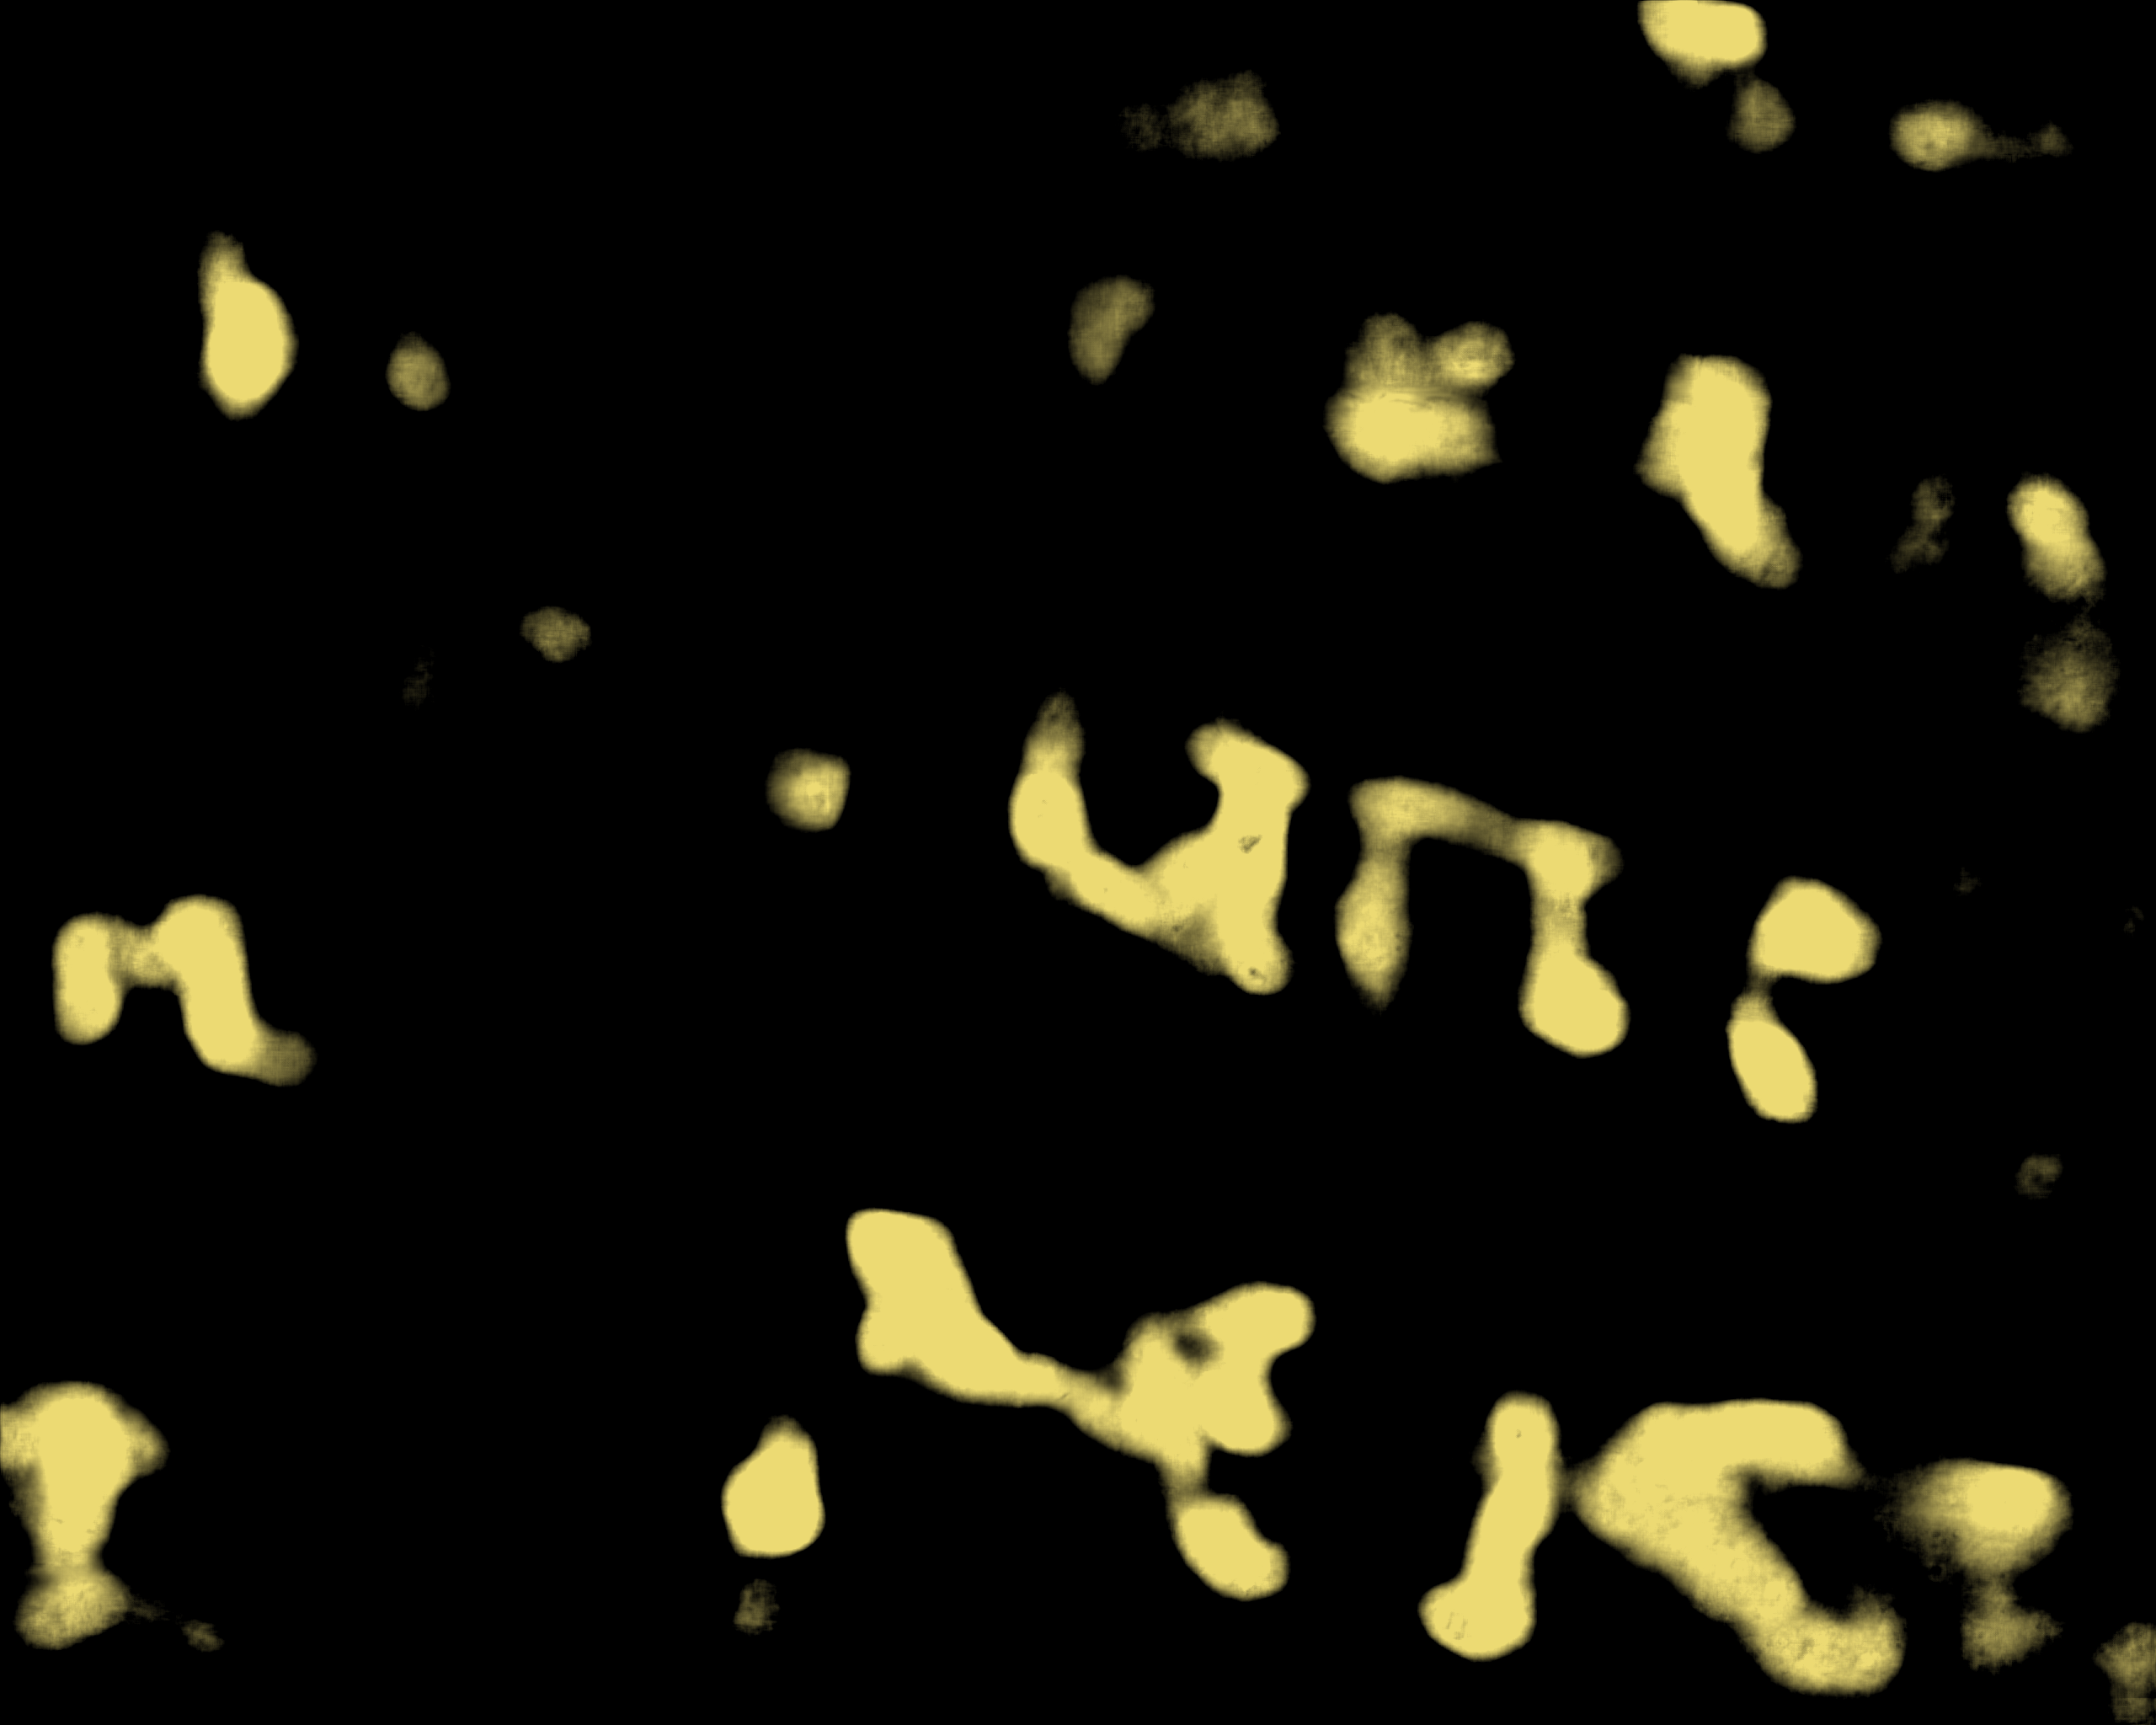
\includegraphics[width=122.48pt]{../figures/w00/w00_6_rectina-m2.png}}\end{minipage}}
\caption{Control unit 0841 w00, three rows of two panels. Row 1: left, Texture; right, Labels. Row 2: left, Reader v2; right, Rectina m1 (display windows: Reader v2 0.419276 to 0.595756 (ramp); Rectina m1 0.577431 to 0.724182 (ramp)). Row 3: left, Reader v3; right, Rectina m2 (display windows: Reader v3 0.454060 to 0.672485 (ramp); Rectina m2 0.650603 to 0.768363 (ramp)). Each map is stretched between its own percentiles. Reader and model stand side by side in the rows 2 and 3.}
\end{figure}

\begin{figure}[!tbp]
\centering
\noindent\makebox[\columnwidth][c]{\begin{minipage}[t]{122.48pt}\centering\href{https://raw.githubusercontent.com/evilaliv3/vesuvius-challenge-pipeline/main/results/db27c806-rectina/src/figures/0343/0343_1_texture.png}{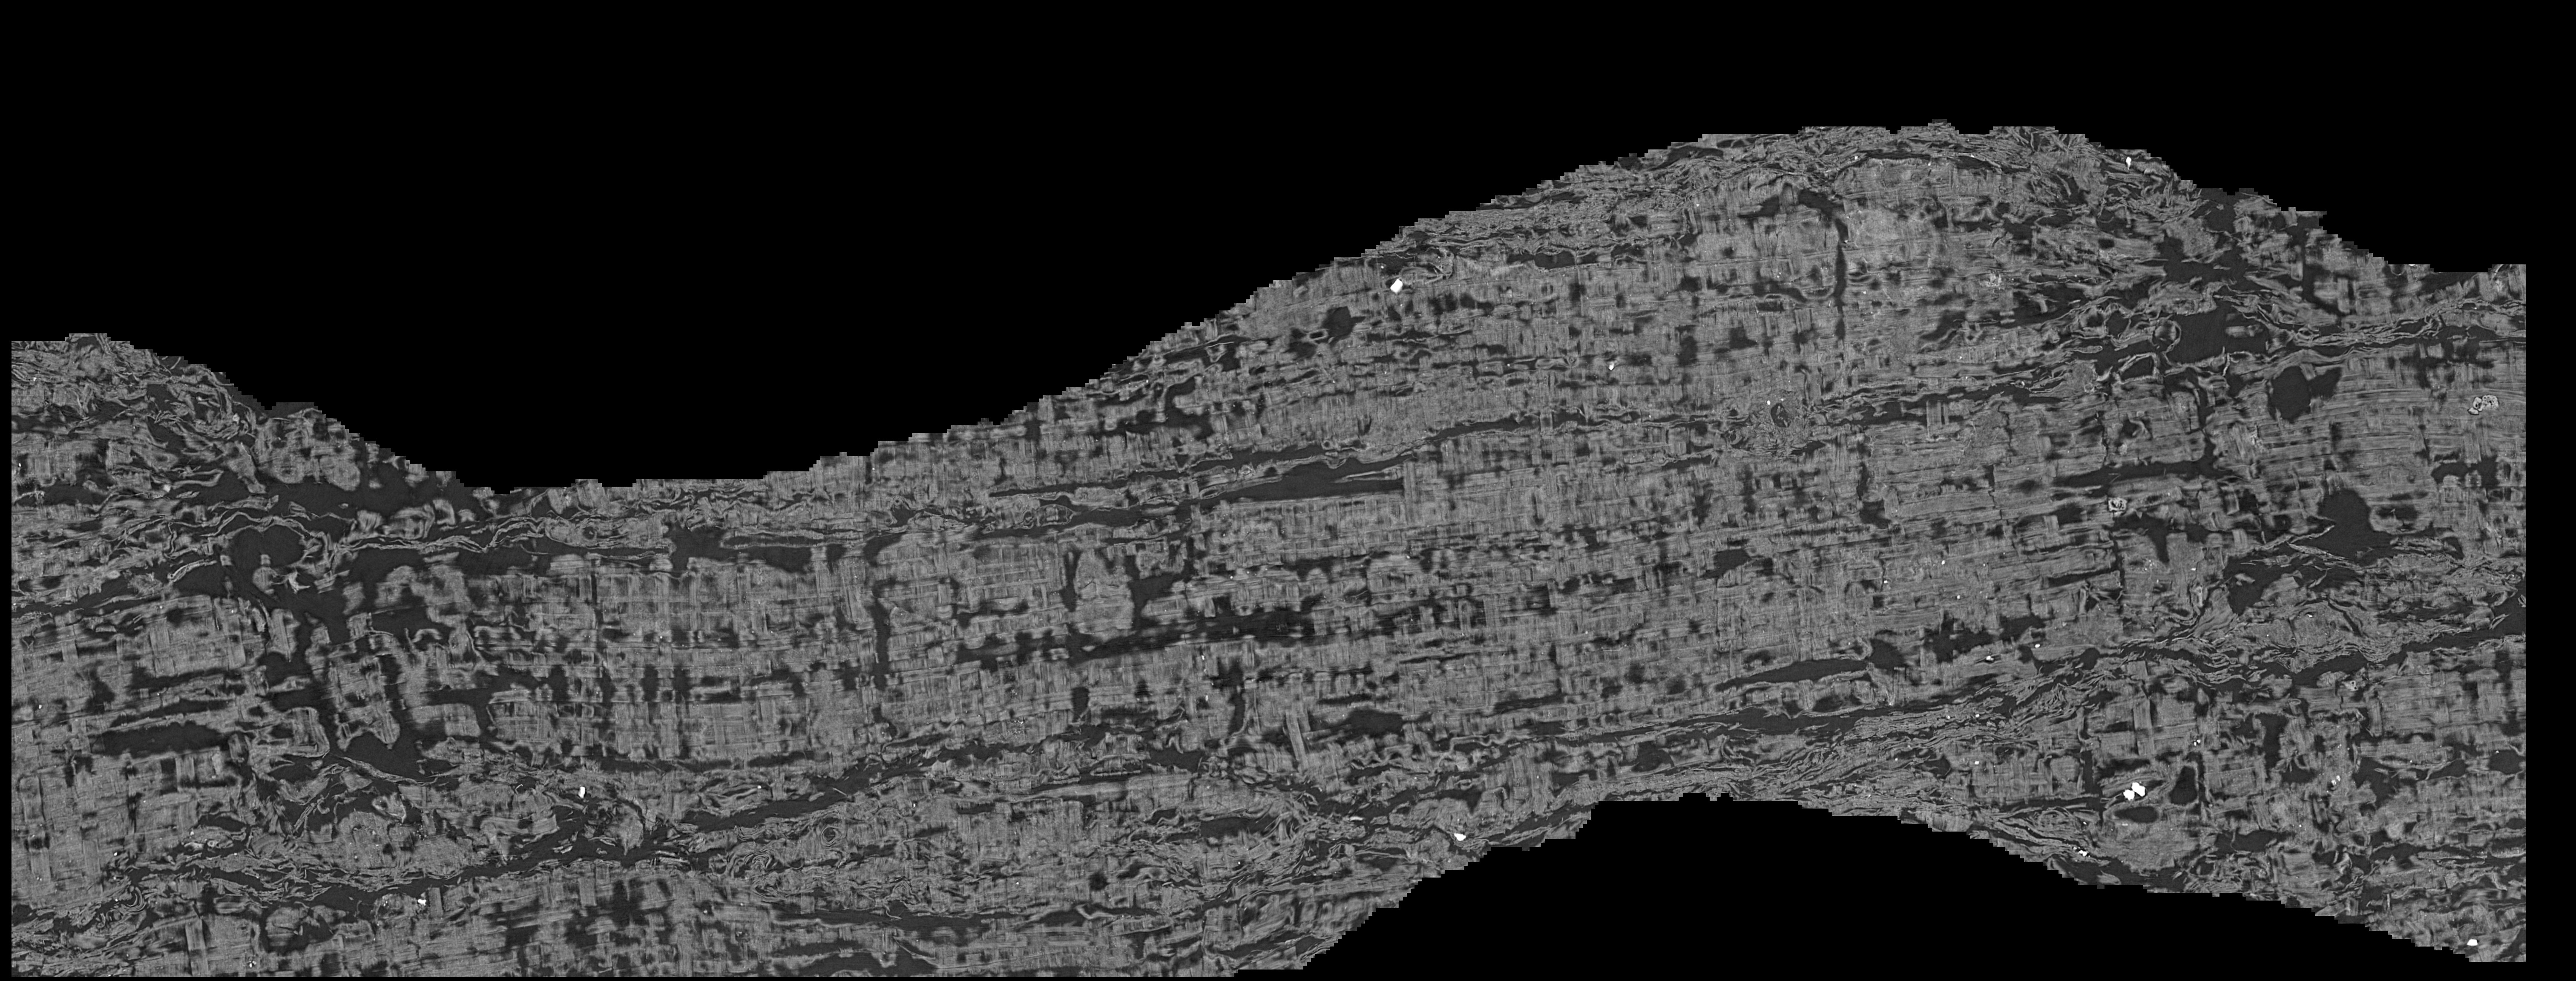
\includegraphics[width=122.48pt]{../figures/0343/0343_1_texture.png}}\end{minipage}\hspace{2pt}\begin{minipage}[t]{122.48pt}\centering\href{https://raw.githubusercontent.com/evilaliv3/vesuvius-challenge-pipeline/main/results/db27c806-rectina/src/figures/0343/0343_2_labels.png}{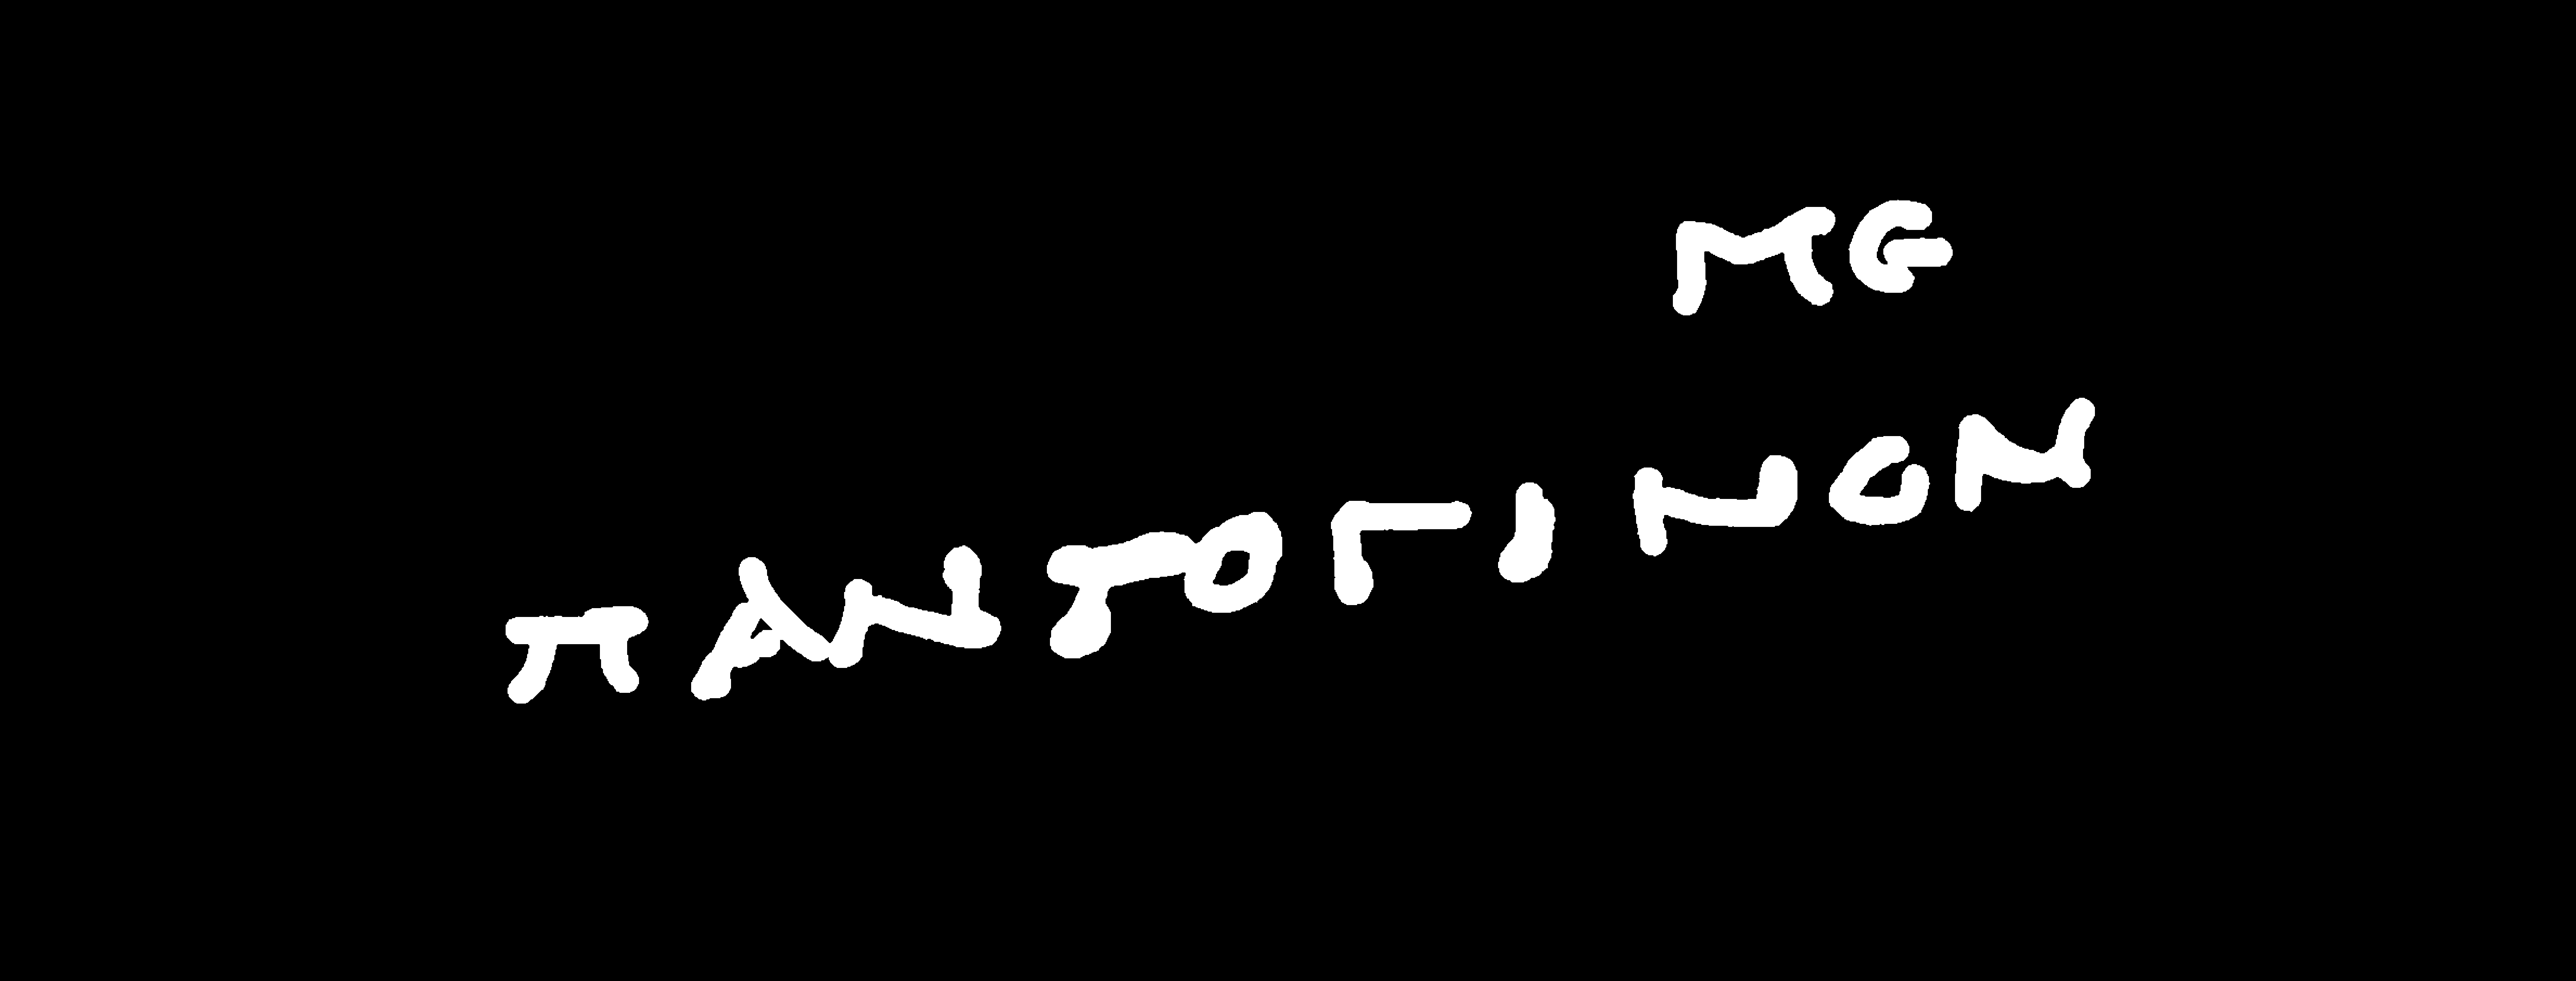
\includegraphics[width=122.48pt]{../figures/0343/0343_2_labels.png}}\end{minipage}}
\par\vspace{4pt}
\noindent\makebox[\columnwidth][c]{\begin{minipage}[t]{122.48pt}\centering\href{https://raw.githubusercontent.com/evilaliv3/vesuvius-challenge-pipeline/main/results/db27c806-rectina/src/figures/0343/0343_3_reader-v2.png}{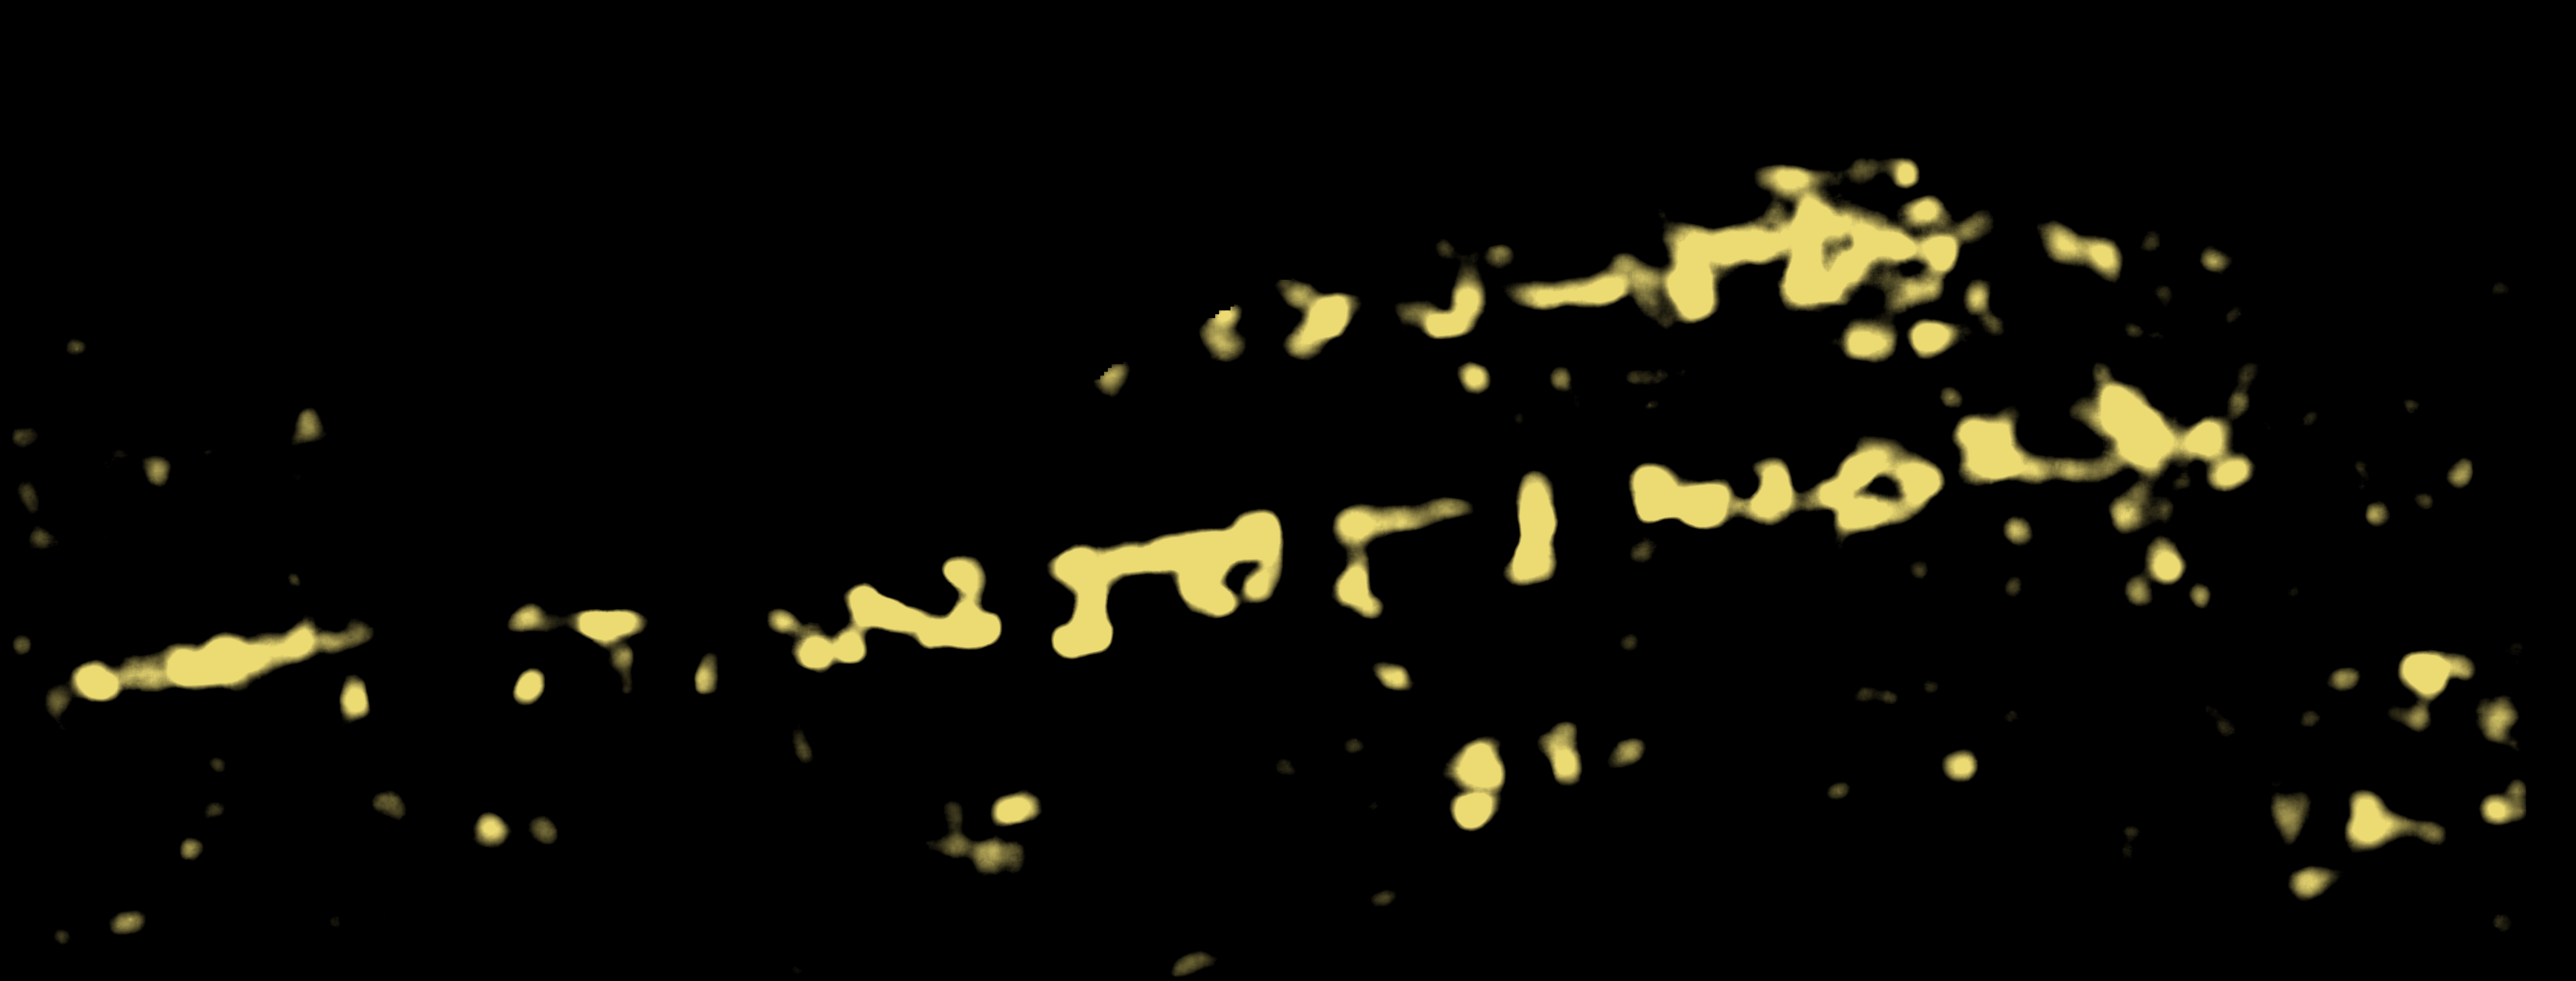
\includegraphics[width=122.48pt]{../figures/0343/0343_3_reader-v2.png}}\end{minipage}\hspace{2pt}\begin{minipage}[t]{122.48pt}\centering\href{https://raw.githubusercontent.com/evilaliv3/vesuvius-challenge-pipeline/main/results/db27c806-rectina/src/figures/0343/0343_5_rectina-m1.png}{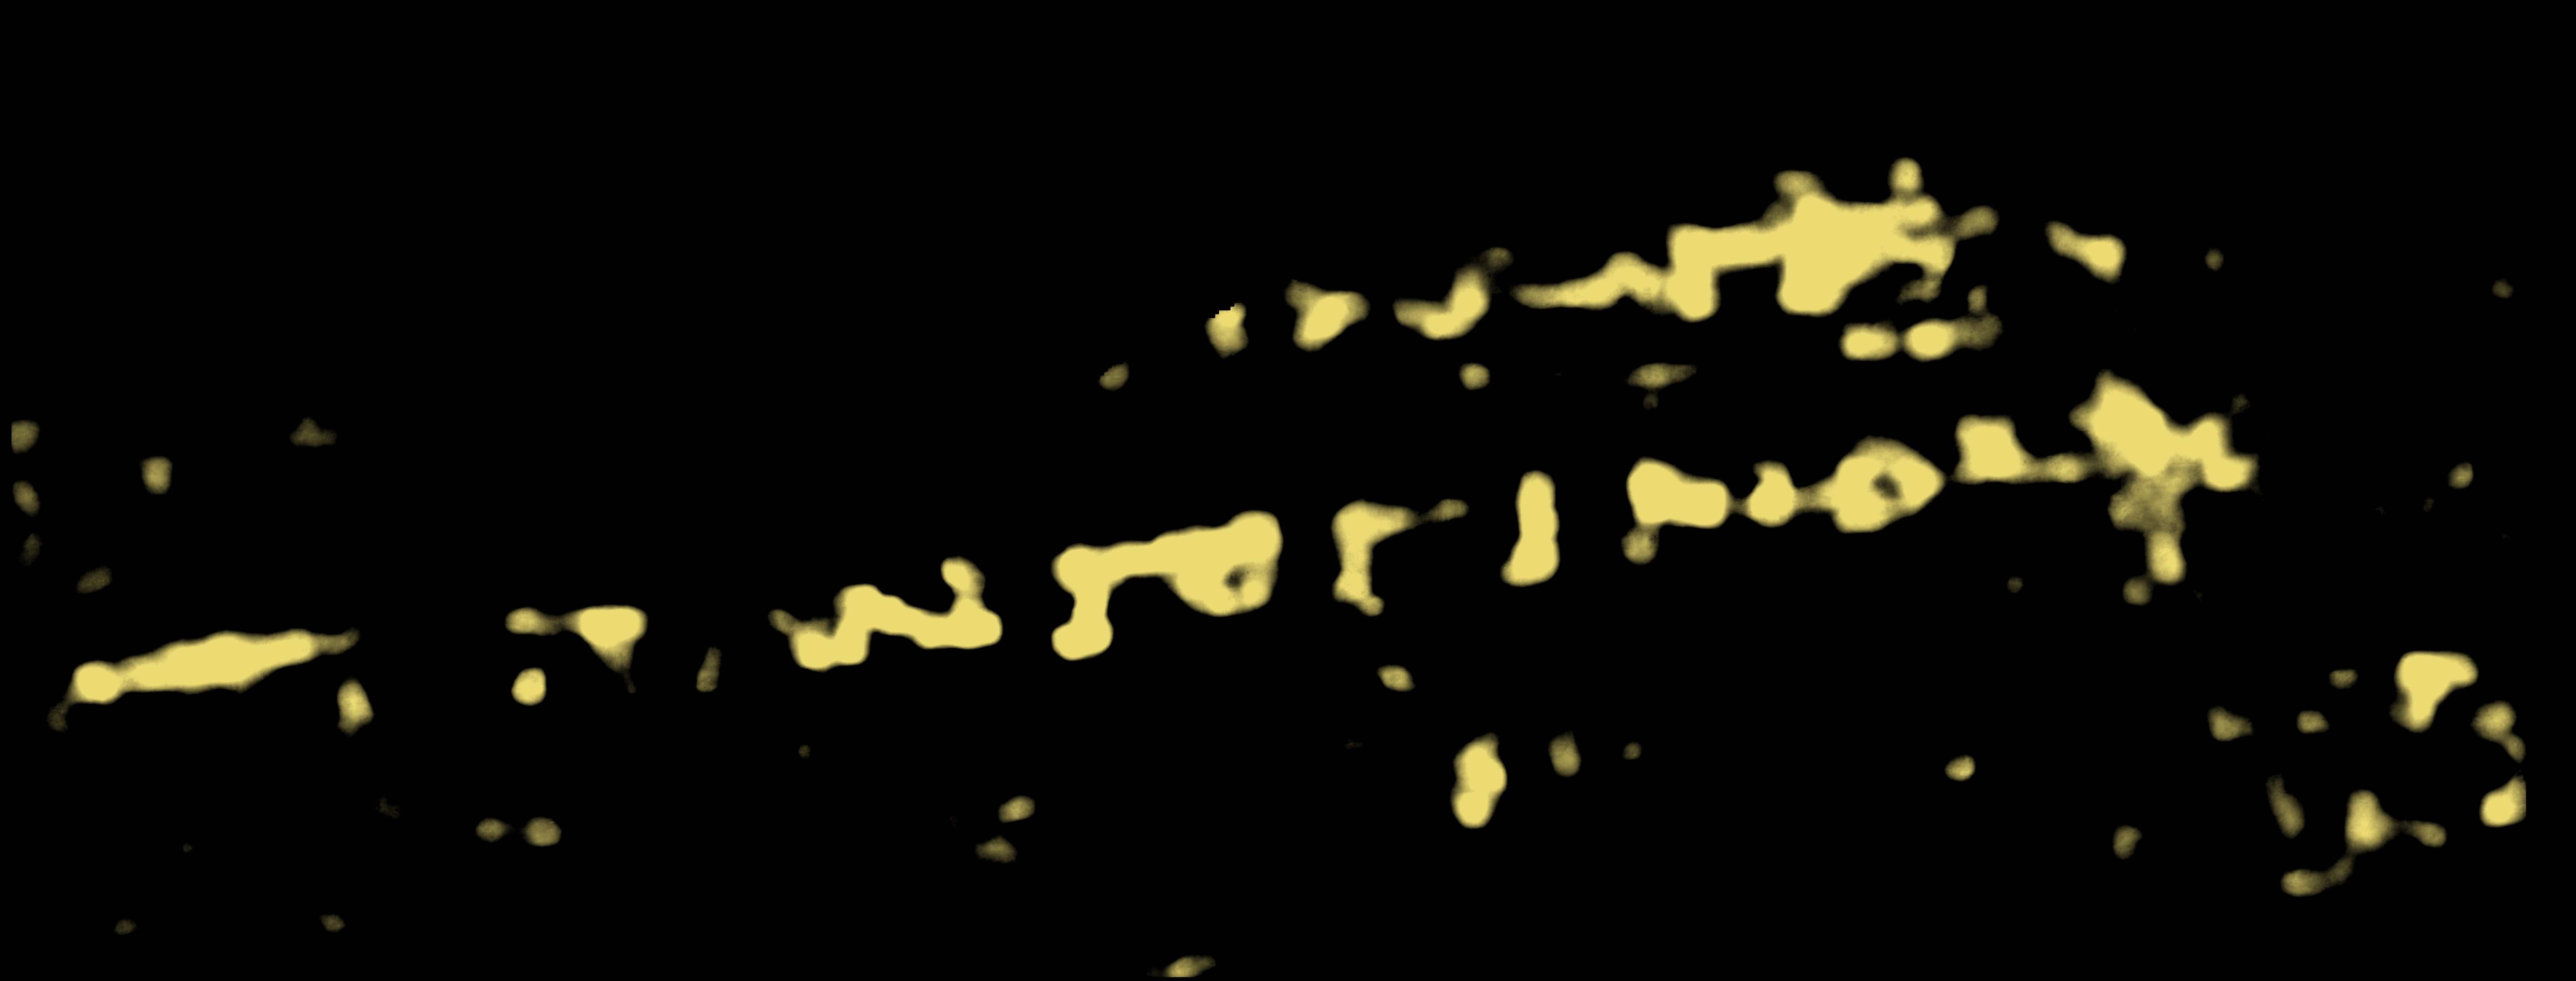
\includegraphics[width=122.48pt]{../figures/0343/0343_5_rectina-m1.png}}\end{minipage}}
\par\vspace{4pt}
\noindent\makebox[\columnwidth][c]{\begin{minipage}[t]{122.48pt}\centering\href{https://raw.githubusercontent.com/evilaliv3/vesuvius-challenge-pipeline/main/results/db27c806-rectina/src/figures/0343/0343_4_reader-v3.png}{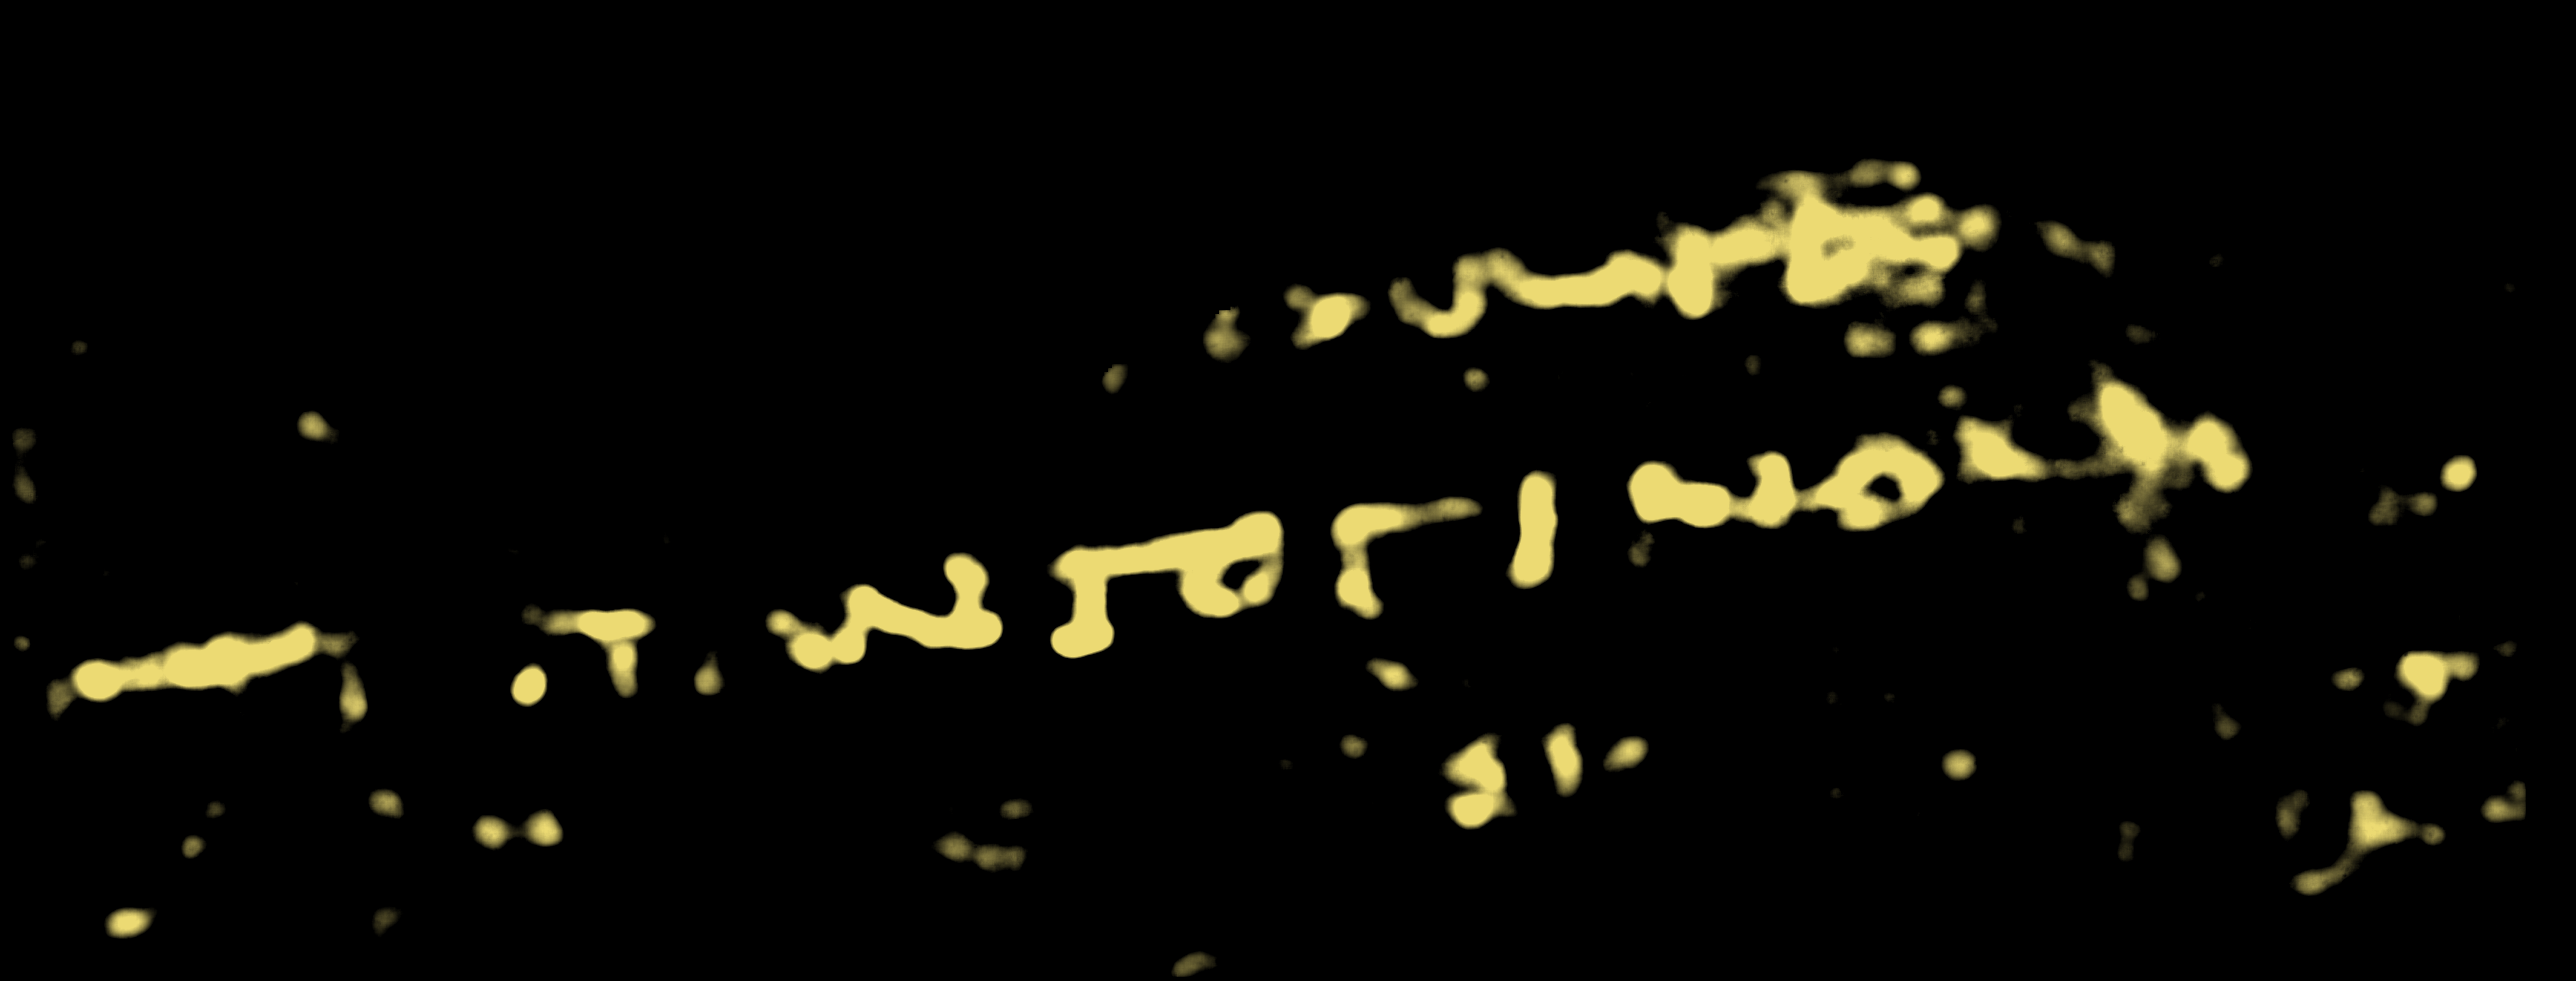
\includegraphics[width=122.48pt]{../figures/0343/0343_4_reader-v3.png}}\end{minipage}\hspace{2pt}\begin{minipage}[t]{122.48pt}\centering\href{https://raw.githubusercontent.com/evilaliv3/vesuvius-challenge-pipeline/main/results/db27c806-rectina/src/figures/0343/0343_6_rectina-m2.png}{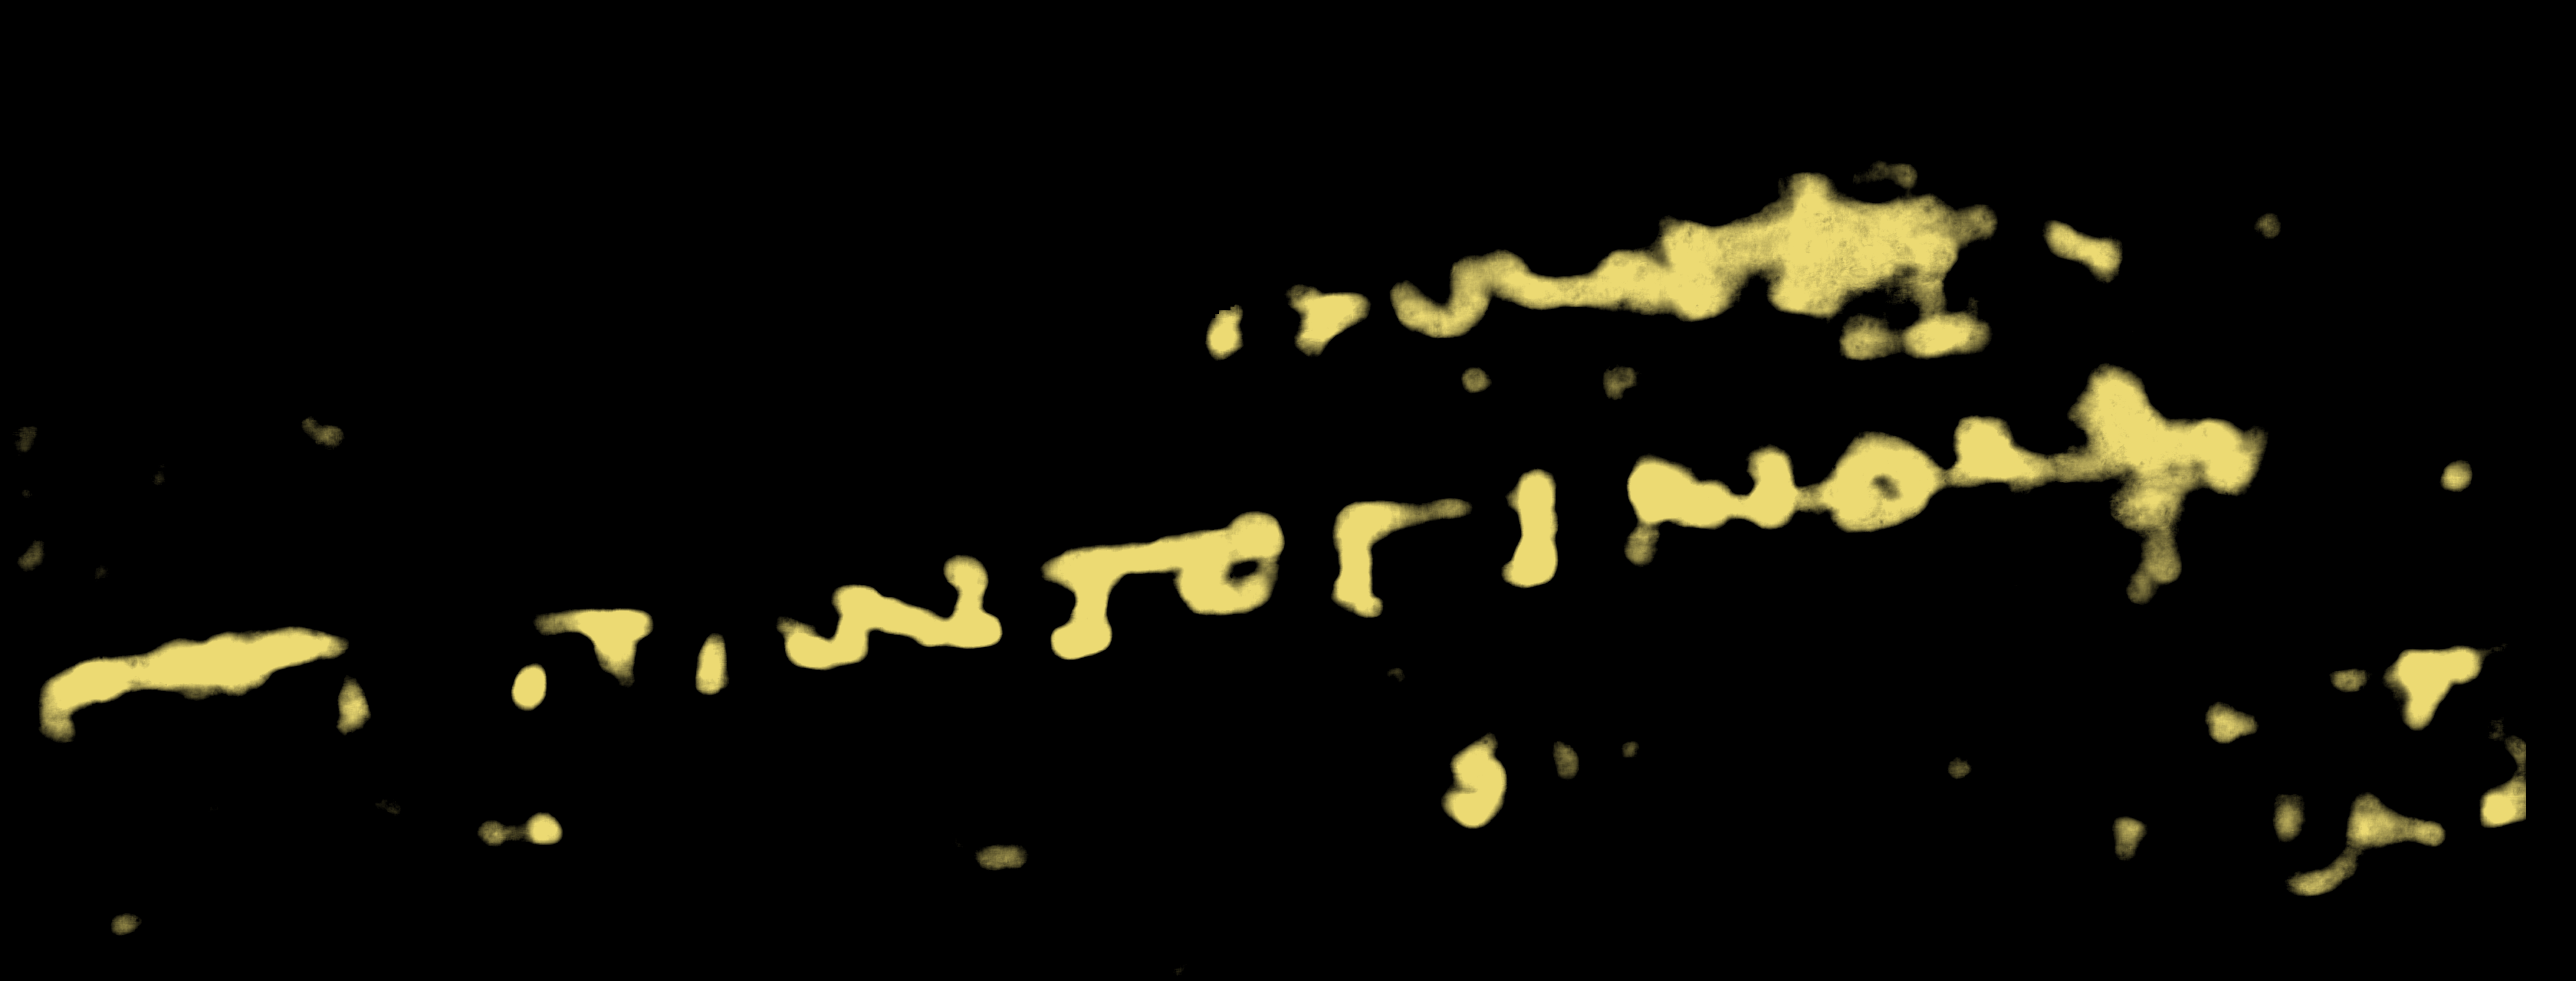
\includegraphics[width=122.48pt]{../figures/0343/0343_6_rectina-m2.png}}\end{minipage}}
\caption{Control unit 0343, three rows of two panels. Row 1: left, Texture; right, Labels. Row 2: left, Reader v2; right, Rectina m1 (display windows: Reader v2 0.409836 to 0.590749 (ramp); Rectina m1 0.548366 to 0.721975 (ramp)). Row 3: left, Reader v3; right, Rectina m2 (display windows: Reader v3 0.444697 to 0.678368 (ramp); Rectina m2 0.627931 to 0.765628 (ramp)). Each map is stretched between its own percentiles. The control is shown rotated 180 degrees, as the index of the panels records. Reader and model stand side by side in the rows 2 and 3.}
\end{figure}

\begin{figure}[!tbp]
\centering
\noindent\makebox[\columnwidth][c]{\begin{minipage}[t]{122.48pt}\centering\href{https://raw.githubusercontent.com/evilaliv3/vesuvius-challenge-pipeline/main/results/db27c806-rectina/src/figures/w058/w058_1_texture.png}{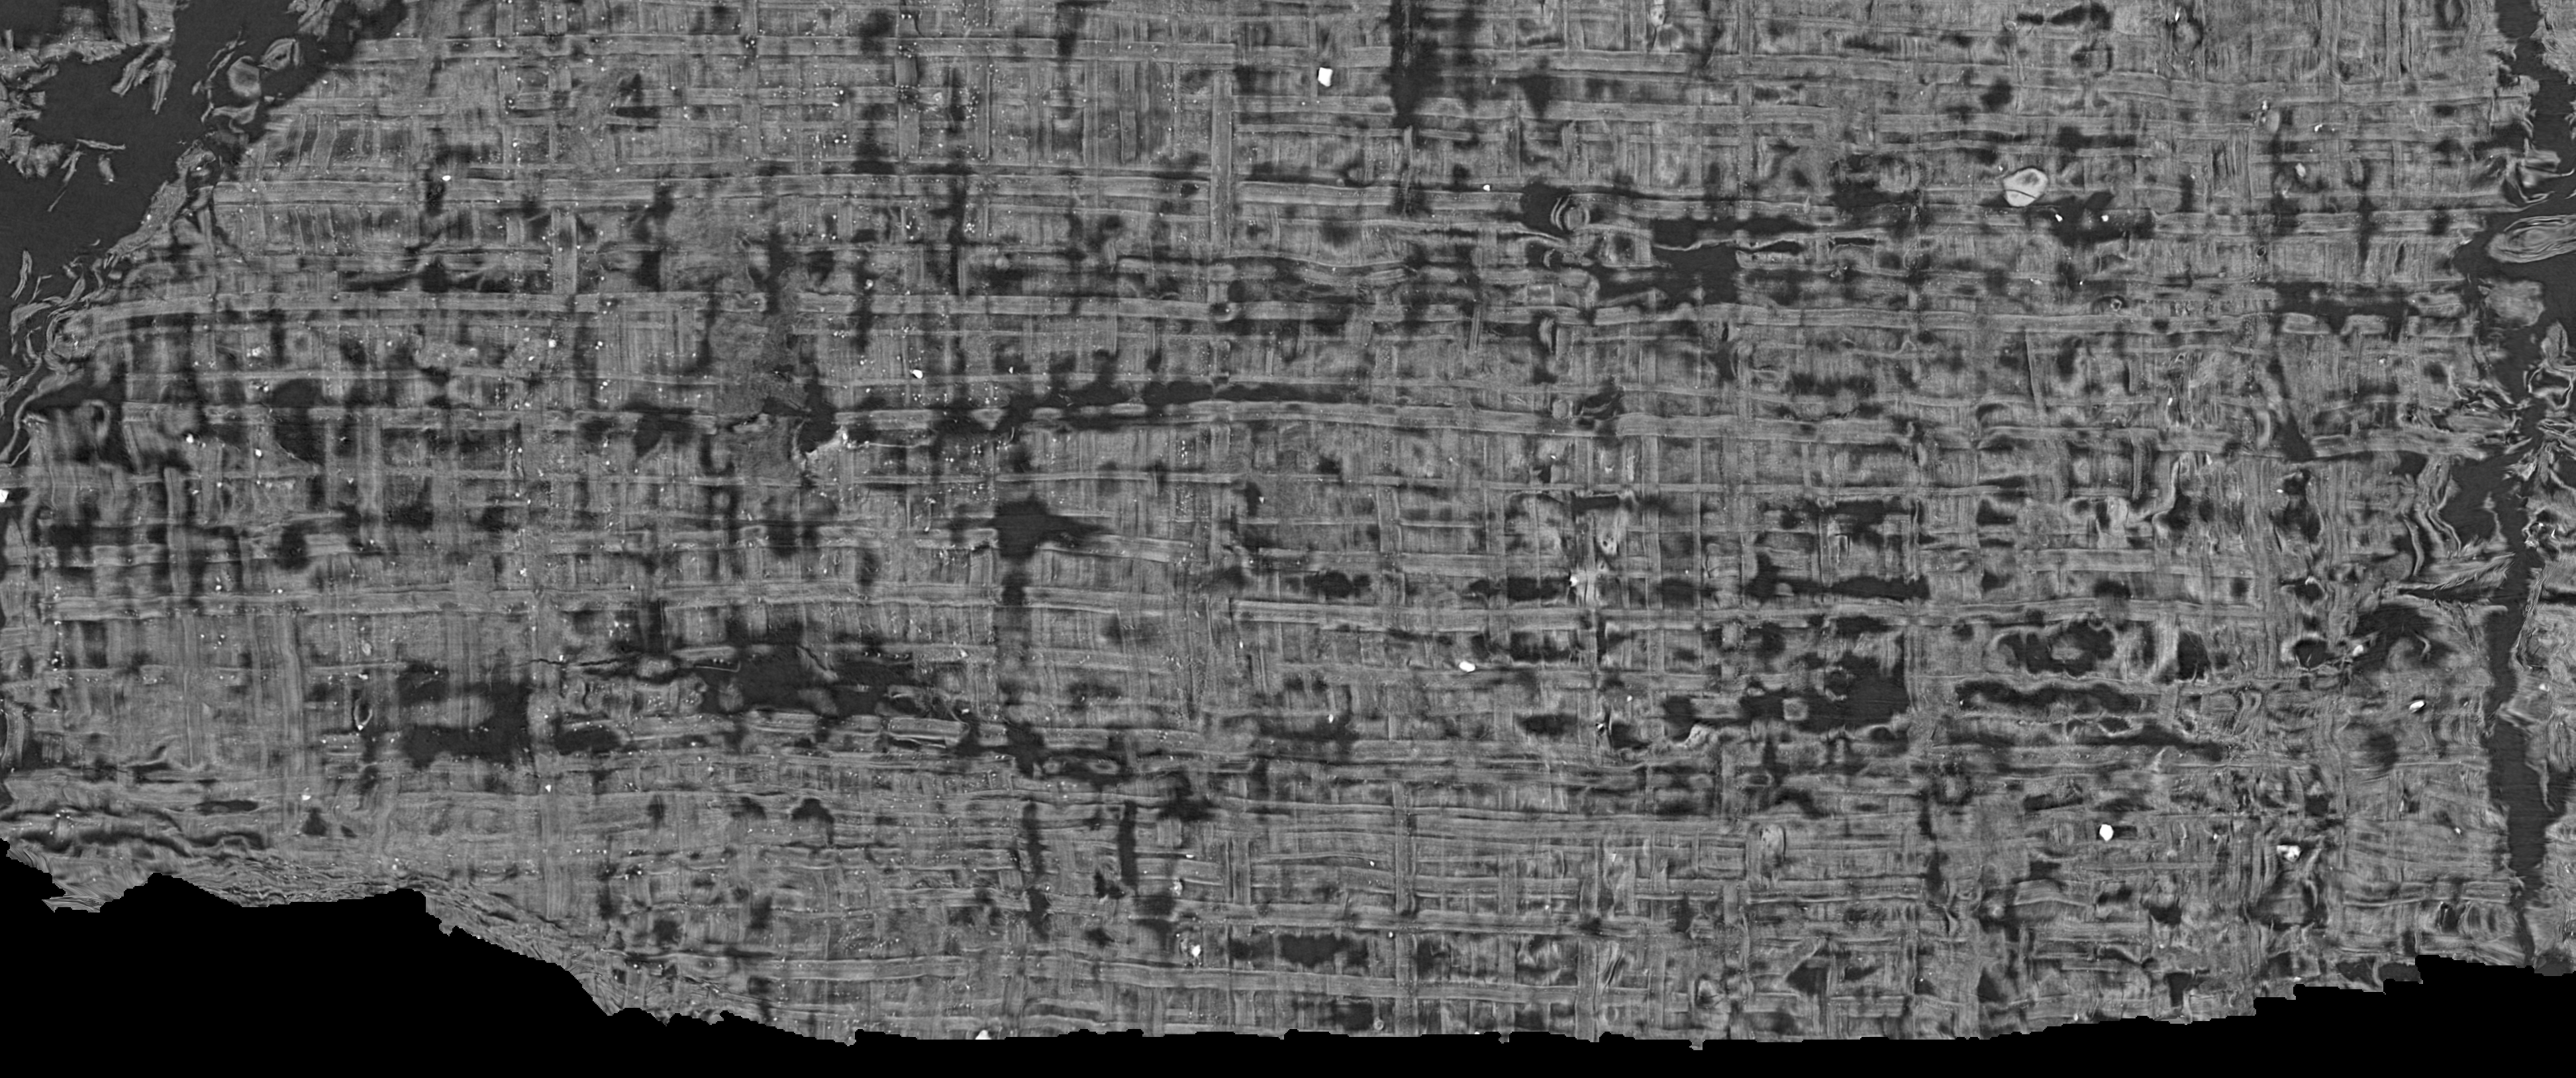
\includegraphics[width=122.48pt]{../figures/w058/w058_1_texture.png}}\end{minipage}\hspace{2pt}\begin{minipage}[t]{122.48pt}\centering\href{https://raw.githubusercontent.com/evilaliv3/vesuvius-challenge-pipeline/main/results/db27c806-rectina/src/figures/w058/w058_2_labels.png}{
\includegraphics[width=122.48pt]{../figures/w058/w058_2_labels.png}}\end{minipage}}
\par\vspace{4pt}
\noindent\makebox[\columnwidth][c]{\begin{minipage}[t]{122.48pt}\centering\href{https://raw.githubusercontent.com/evilaliv3/vesuvius-challenge-pipeline/main/results/db27c806-rectina/src/figures/w058/w058_3_reader-v2.png}{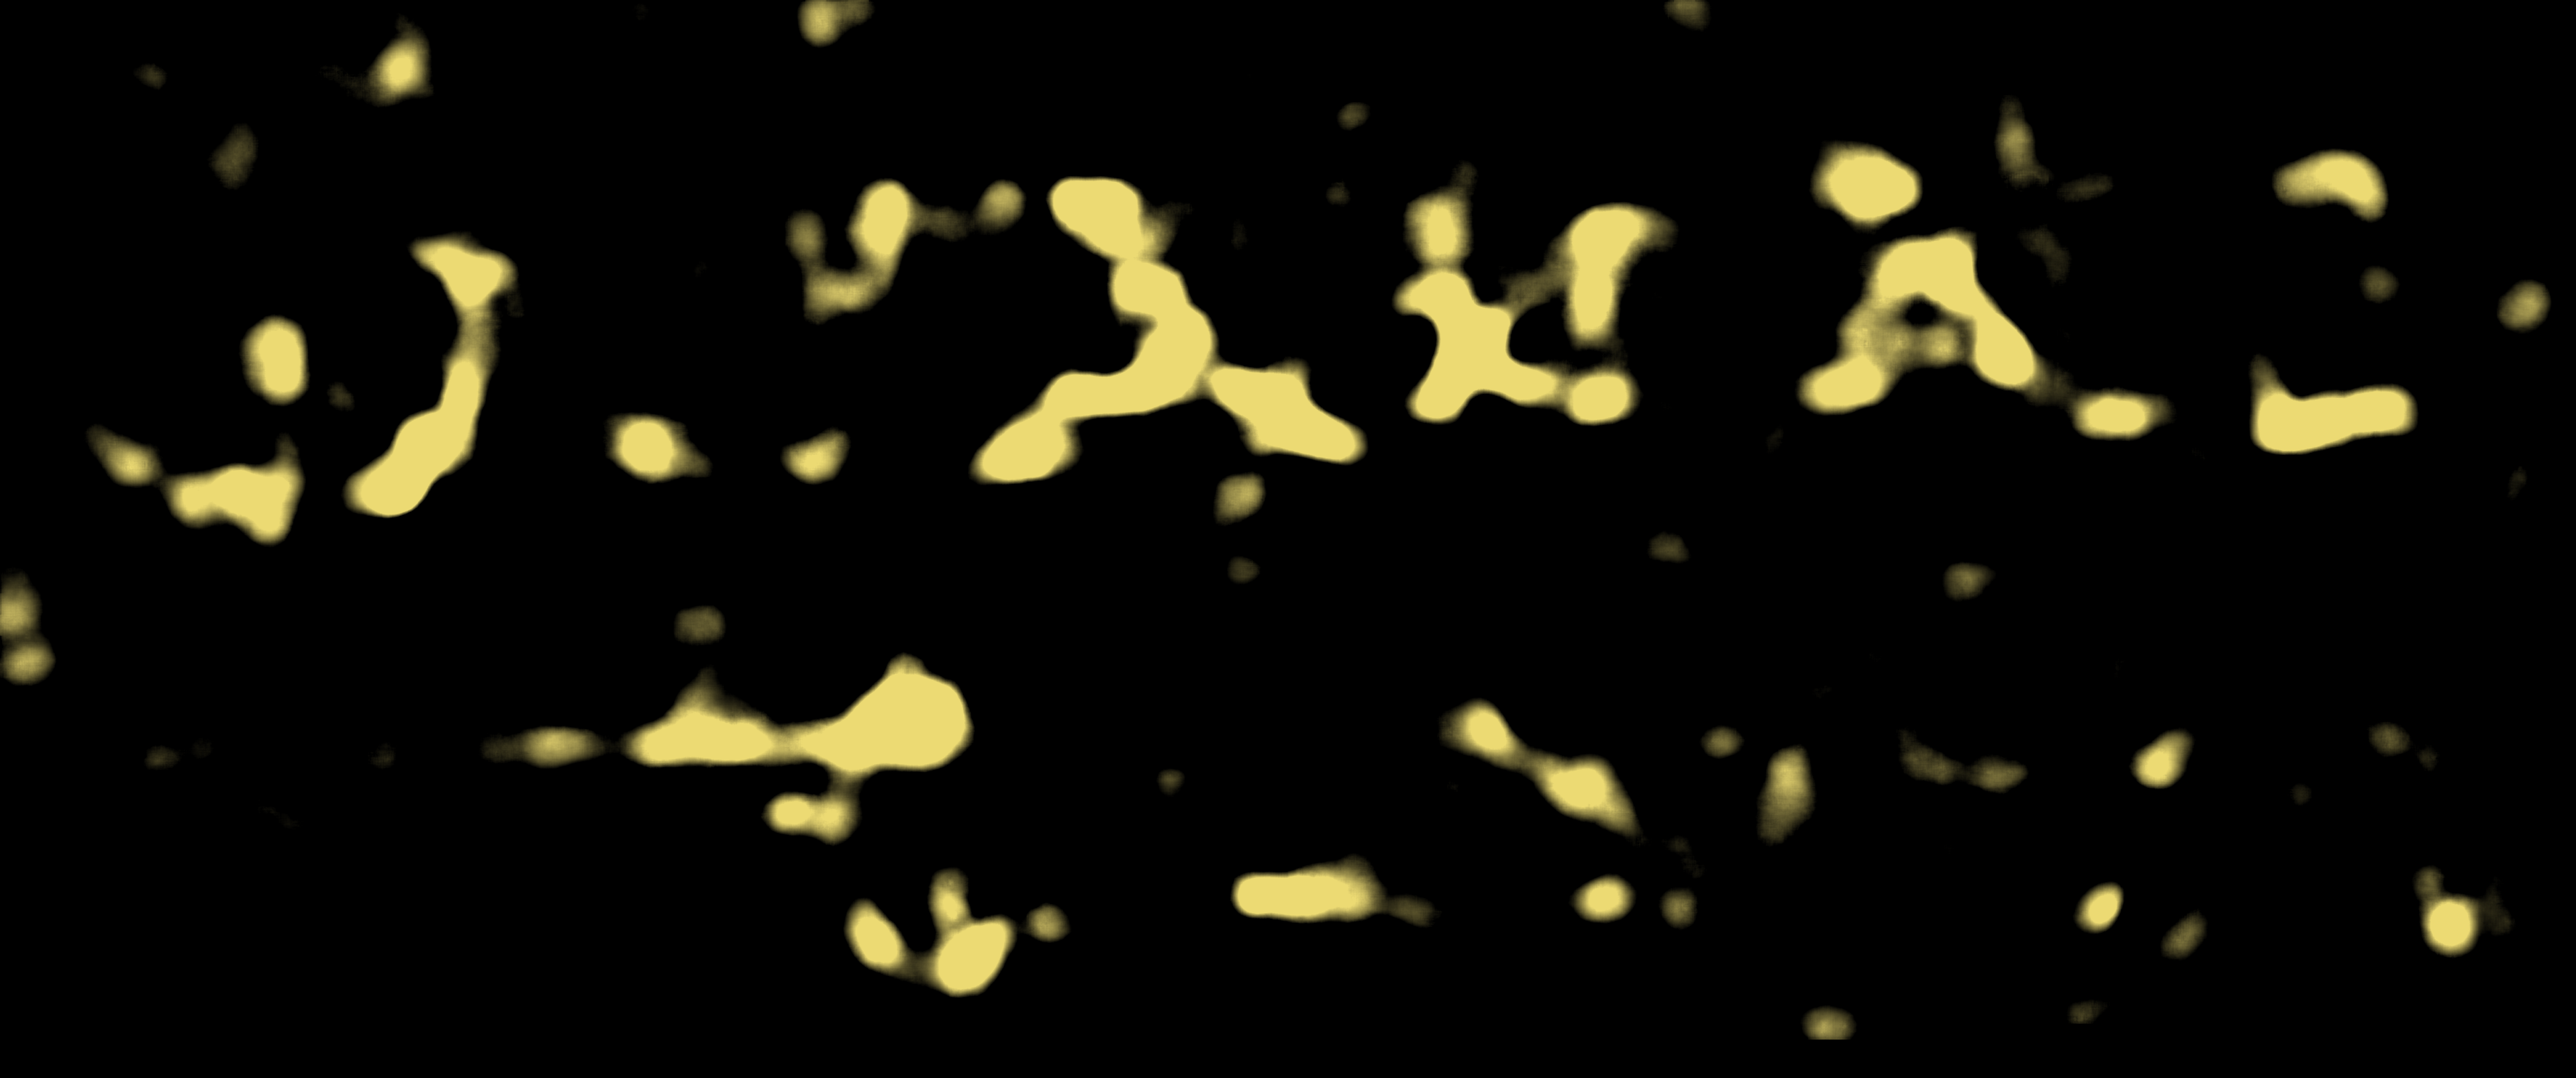
\includegraphics[width=122.48pt]{../figures/w058/w058_3_reader-v2.png}}\end{minipage}\hspace{2pt}\begin{minipage}[t]{122.48pt}\centering\href{https://raw.githubusercontent.com/evilaliv3/vesuvius-challenge-pipeline/main/results/db27c806-rectina/src/figures/w058/w058_5_rectina-m1.png}{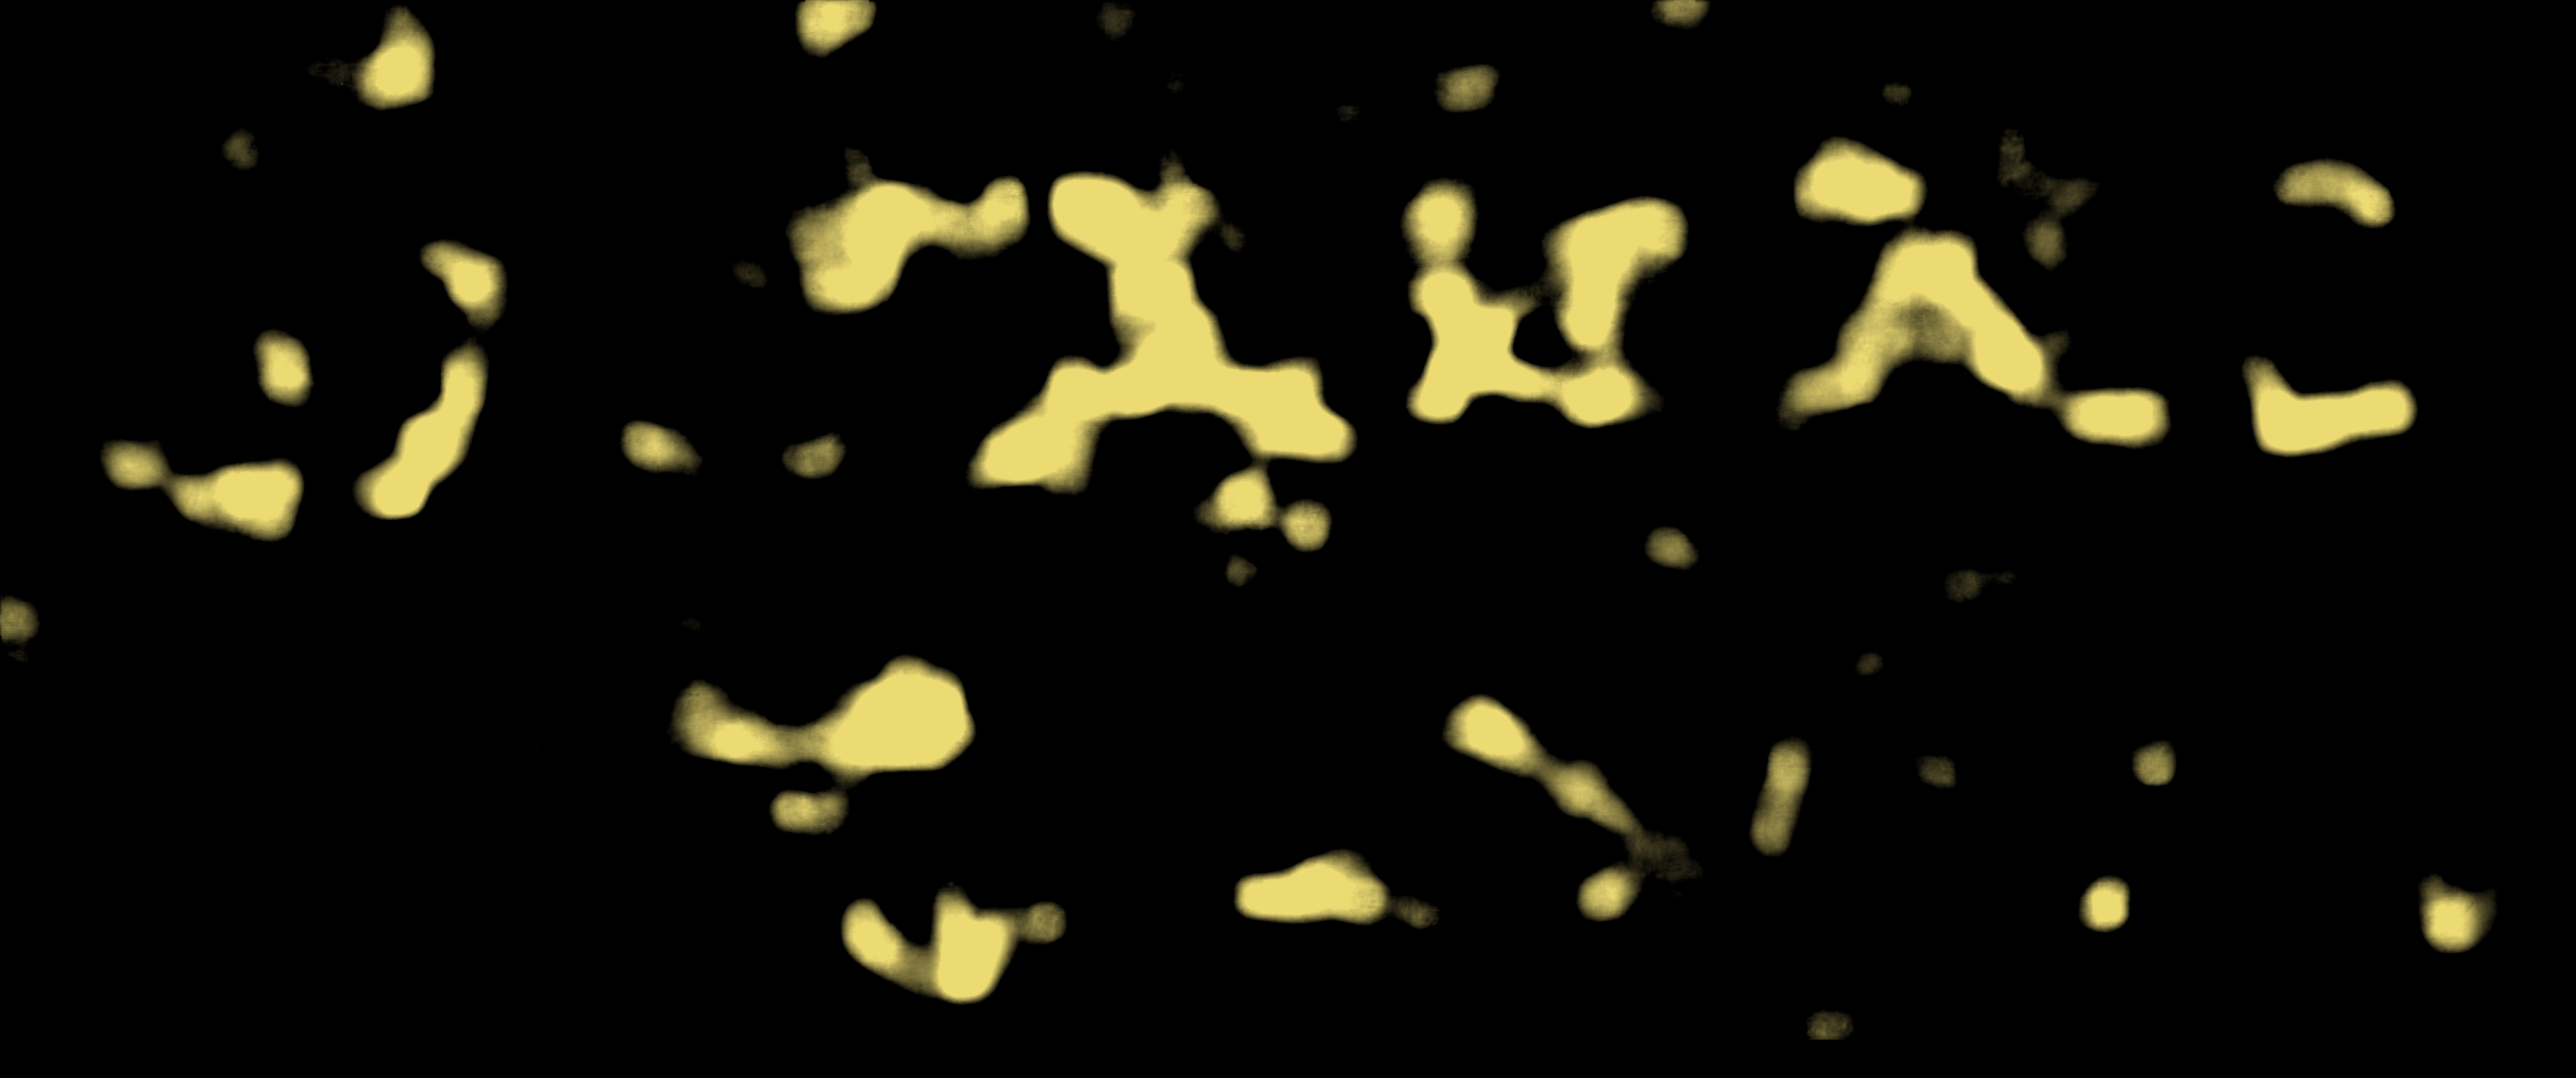
\includegraphics[width=122.48pt]{../figures/w058/w058_5_rectina-m1.png}}\end{minipage}}
\par\vspace{4pt}
\noindent\makebox[\columnwidth][c]{\begin{minipage}[t]{122.48pt}\centering\href{https://raw.githubusercontent.com/evilaliv3/vesuvius-challenge-pipeline/main/results/db27c806-rectina/src/figures/w058/w058_4_reader-v3.png}{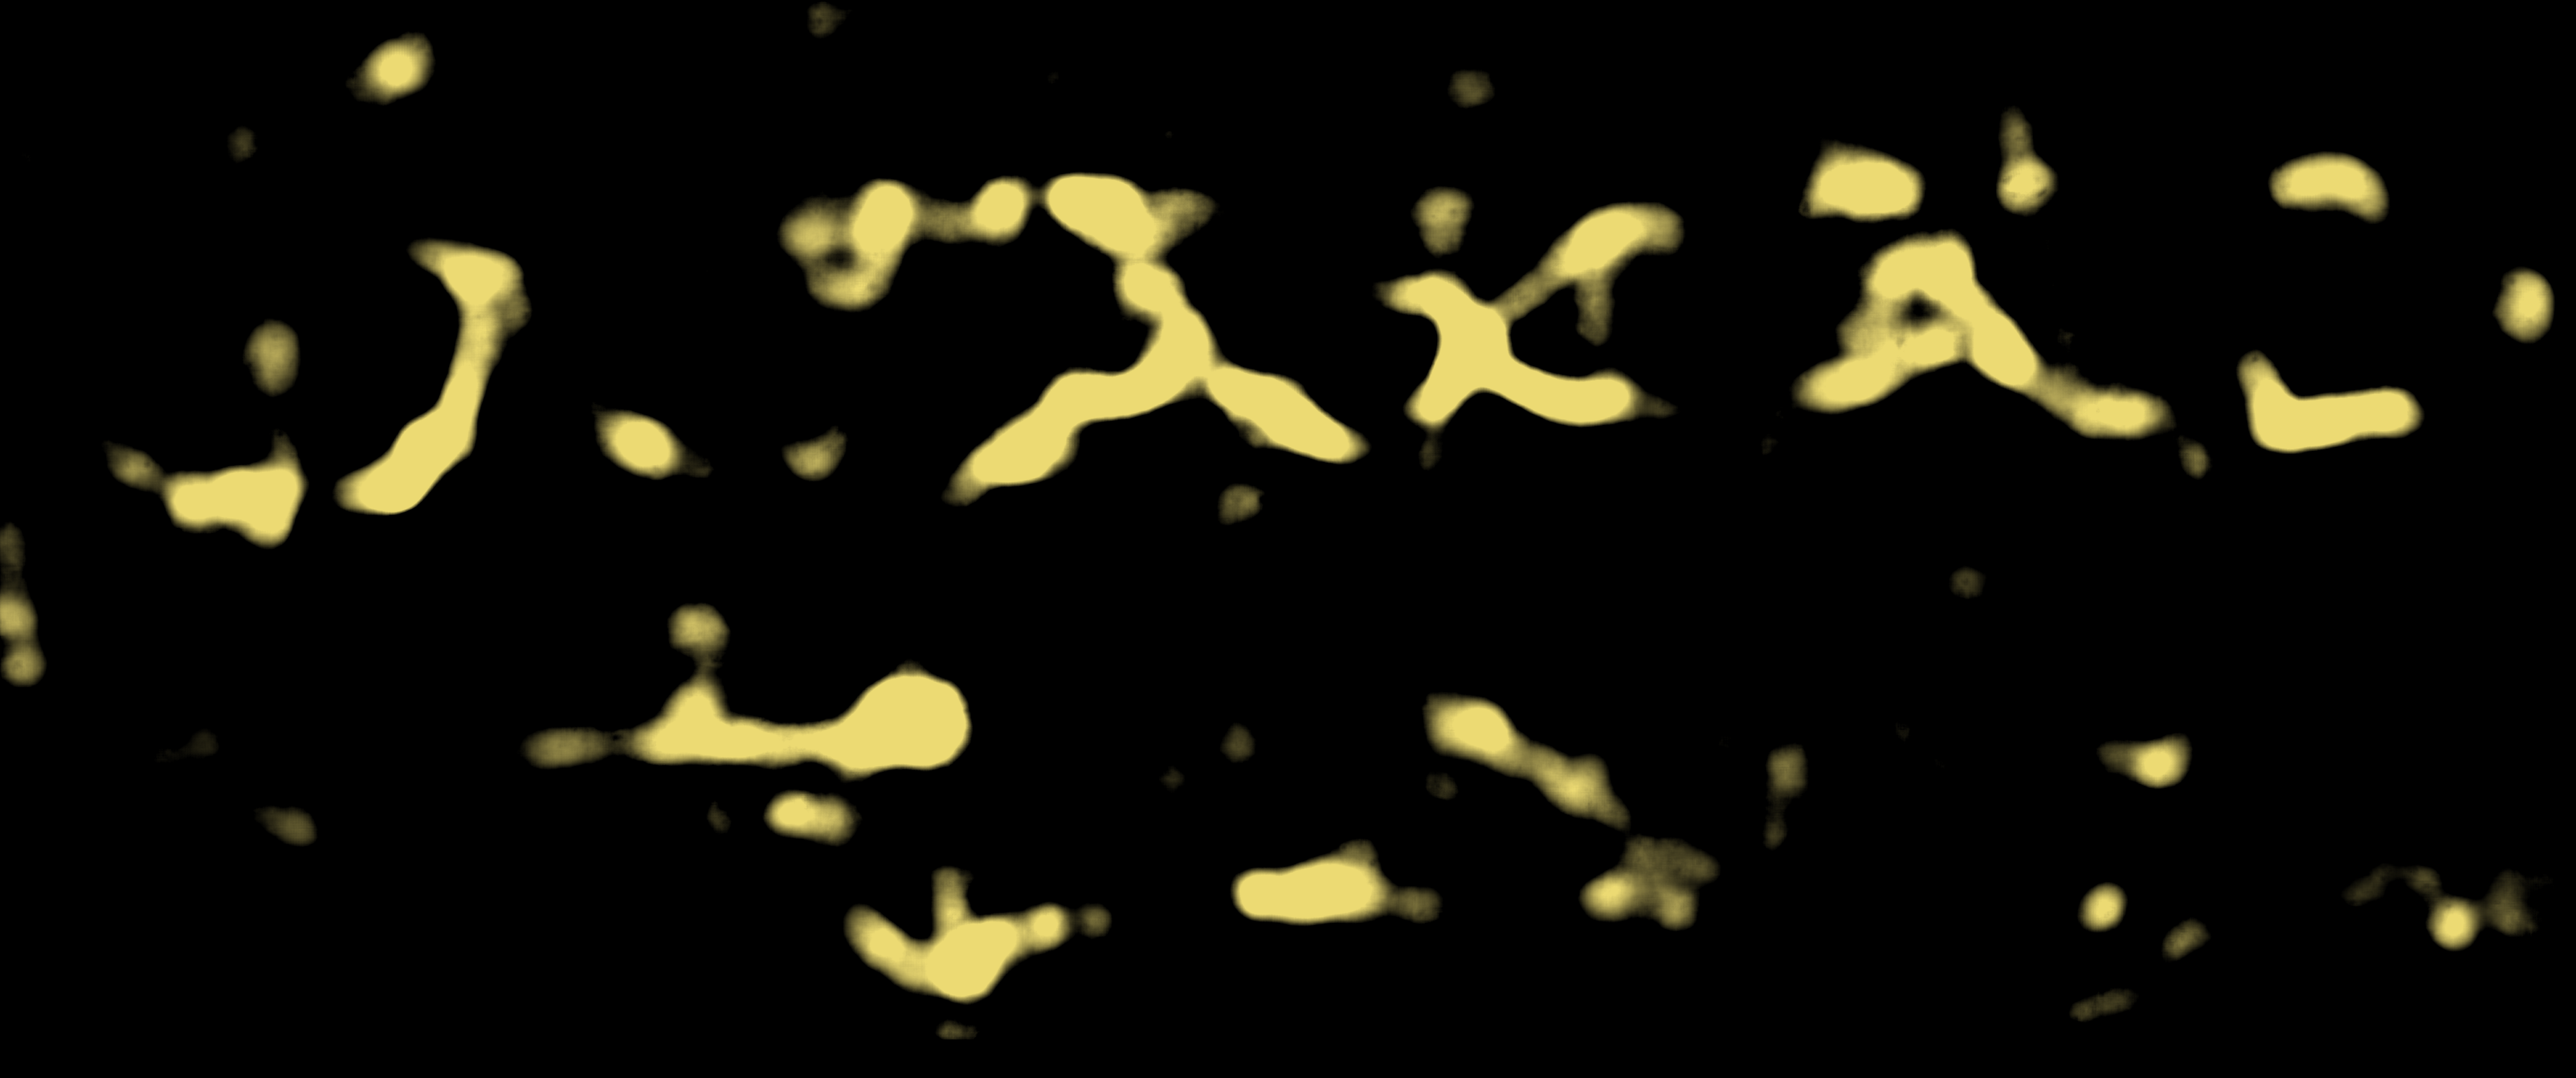
\includegraphics[width=122.48pt]{../figures/w058/w058_4_reader-v3.png}}\end{minipage}\hspace{2pt}\begin{minipage}[t]{122.48pt}\centering\href{https://raw.githubusercontent.com/evilaliv3/vesuvius-challenge-pipeline/main/results/db27c806-rectina/src/figures/w058/w058_6_rectina-m2.png}{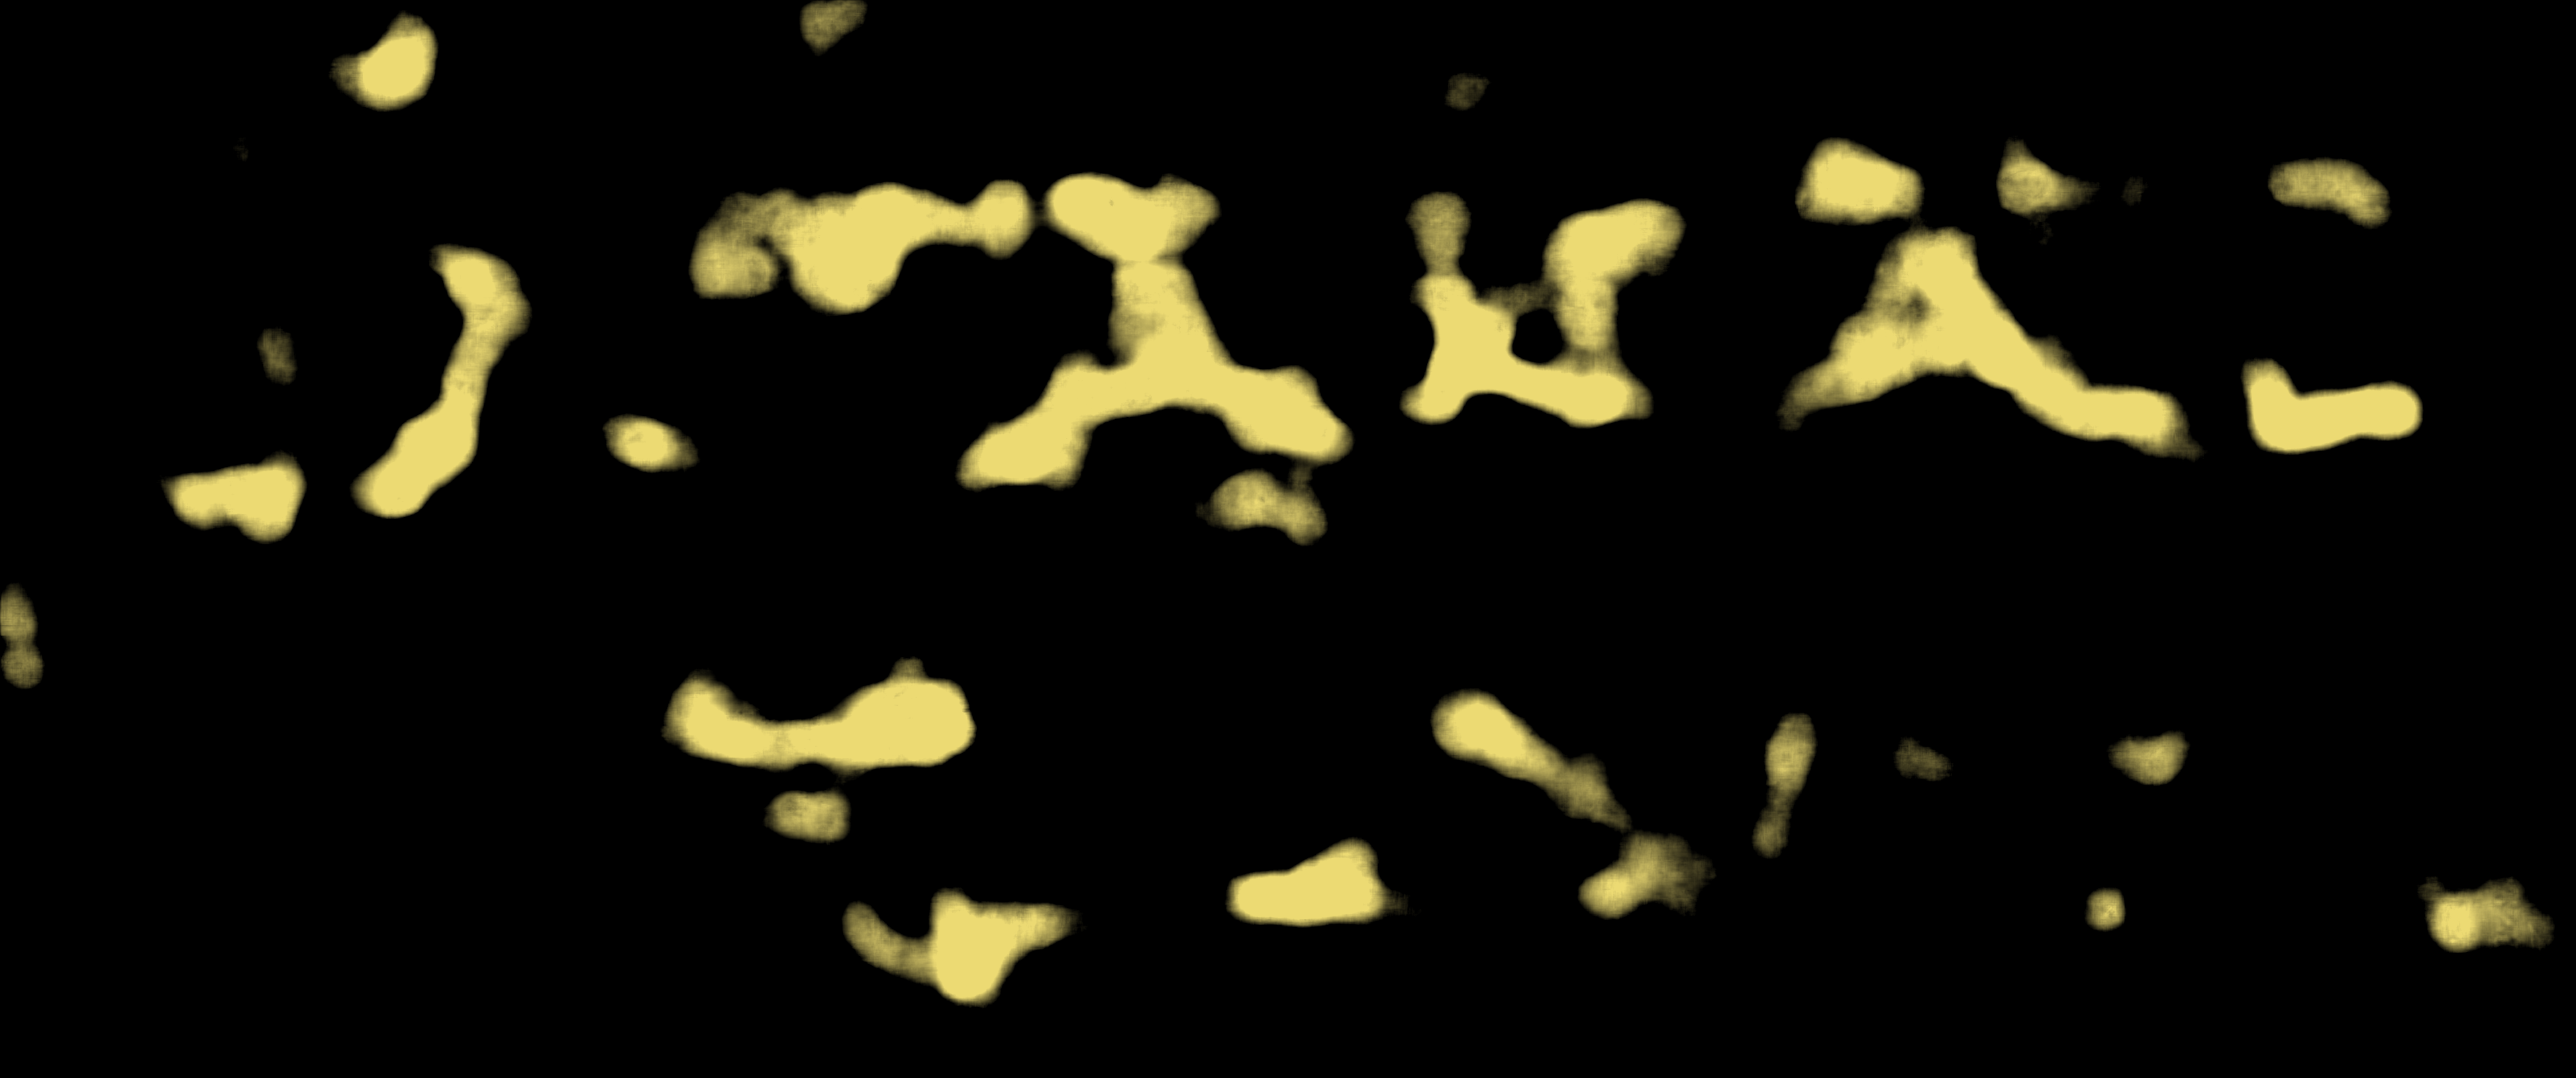
\includegraphics[width=122.48pt]{../figures/w058/w058_6_rectina-m2.png}}\end{minipage}}
\caption{Control unit 1447 w058, three rows of two panels. Row 1: left, Texture; right, Labels. Row 2: left, Reader v2; right, Rectina m1 (display windows: Reader v2 0.385394 to 0.561662 (ramp); Rectina m1 0.533701 to 0.711716 (ramp)). Row 3: left, Reader v3; right, Rectina m2 (display windows: Reader v3 0.450583 to 0.670398 (ramp); Rectina m2 0.625307 to 0.773366 (ramp)). Each map is stretched between its own percentiles. Reader and model stand side by side in the rows 2 and 3.}
\end{figure}

\begin{figure}[!tbp]
\centering
\noindent\makebox[\columnwidth][c]{\begin{minipage}[t]{122.48pt}\centering\href{https://raw.githubusercontent.com/evilaliv3/vesuvius-challenge-pipeline/main/results/db27c806-rectina/src/figures/w060/w060_1_texture.png}{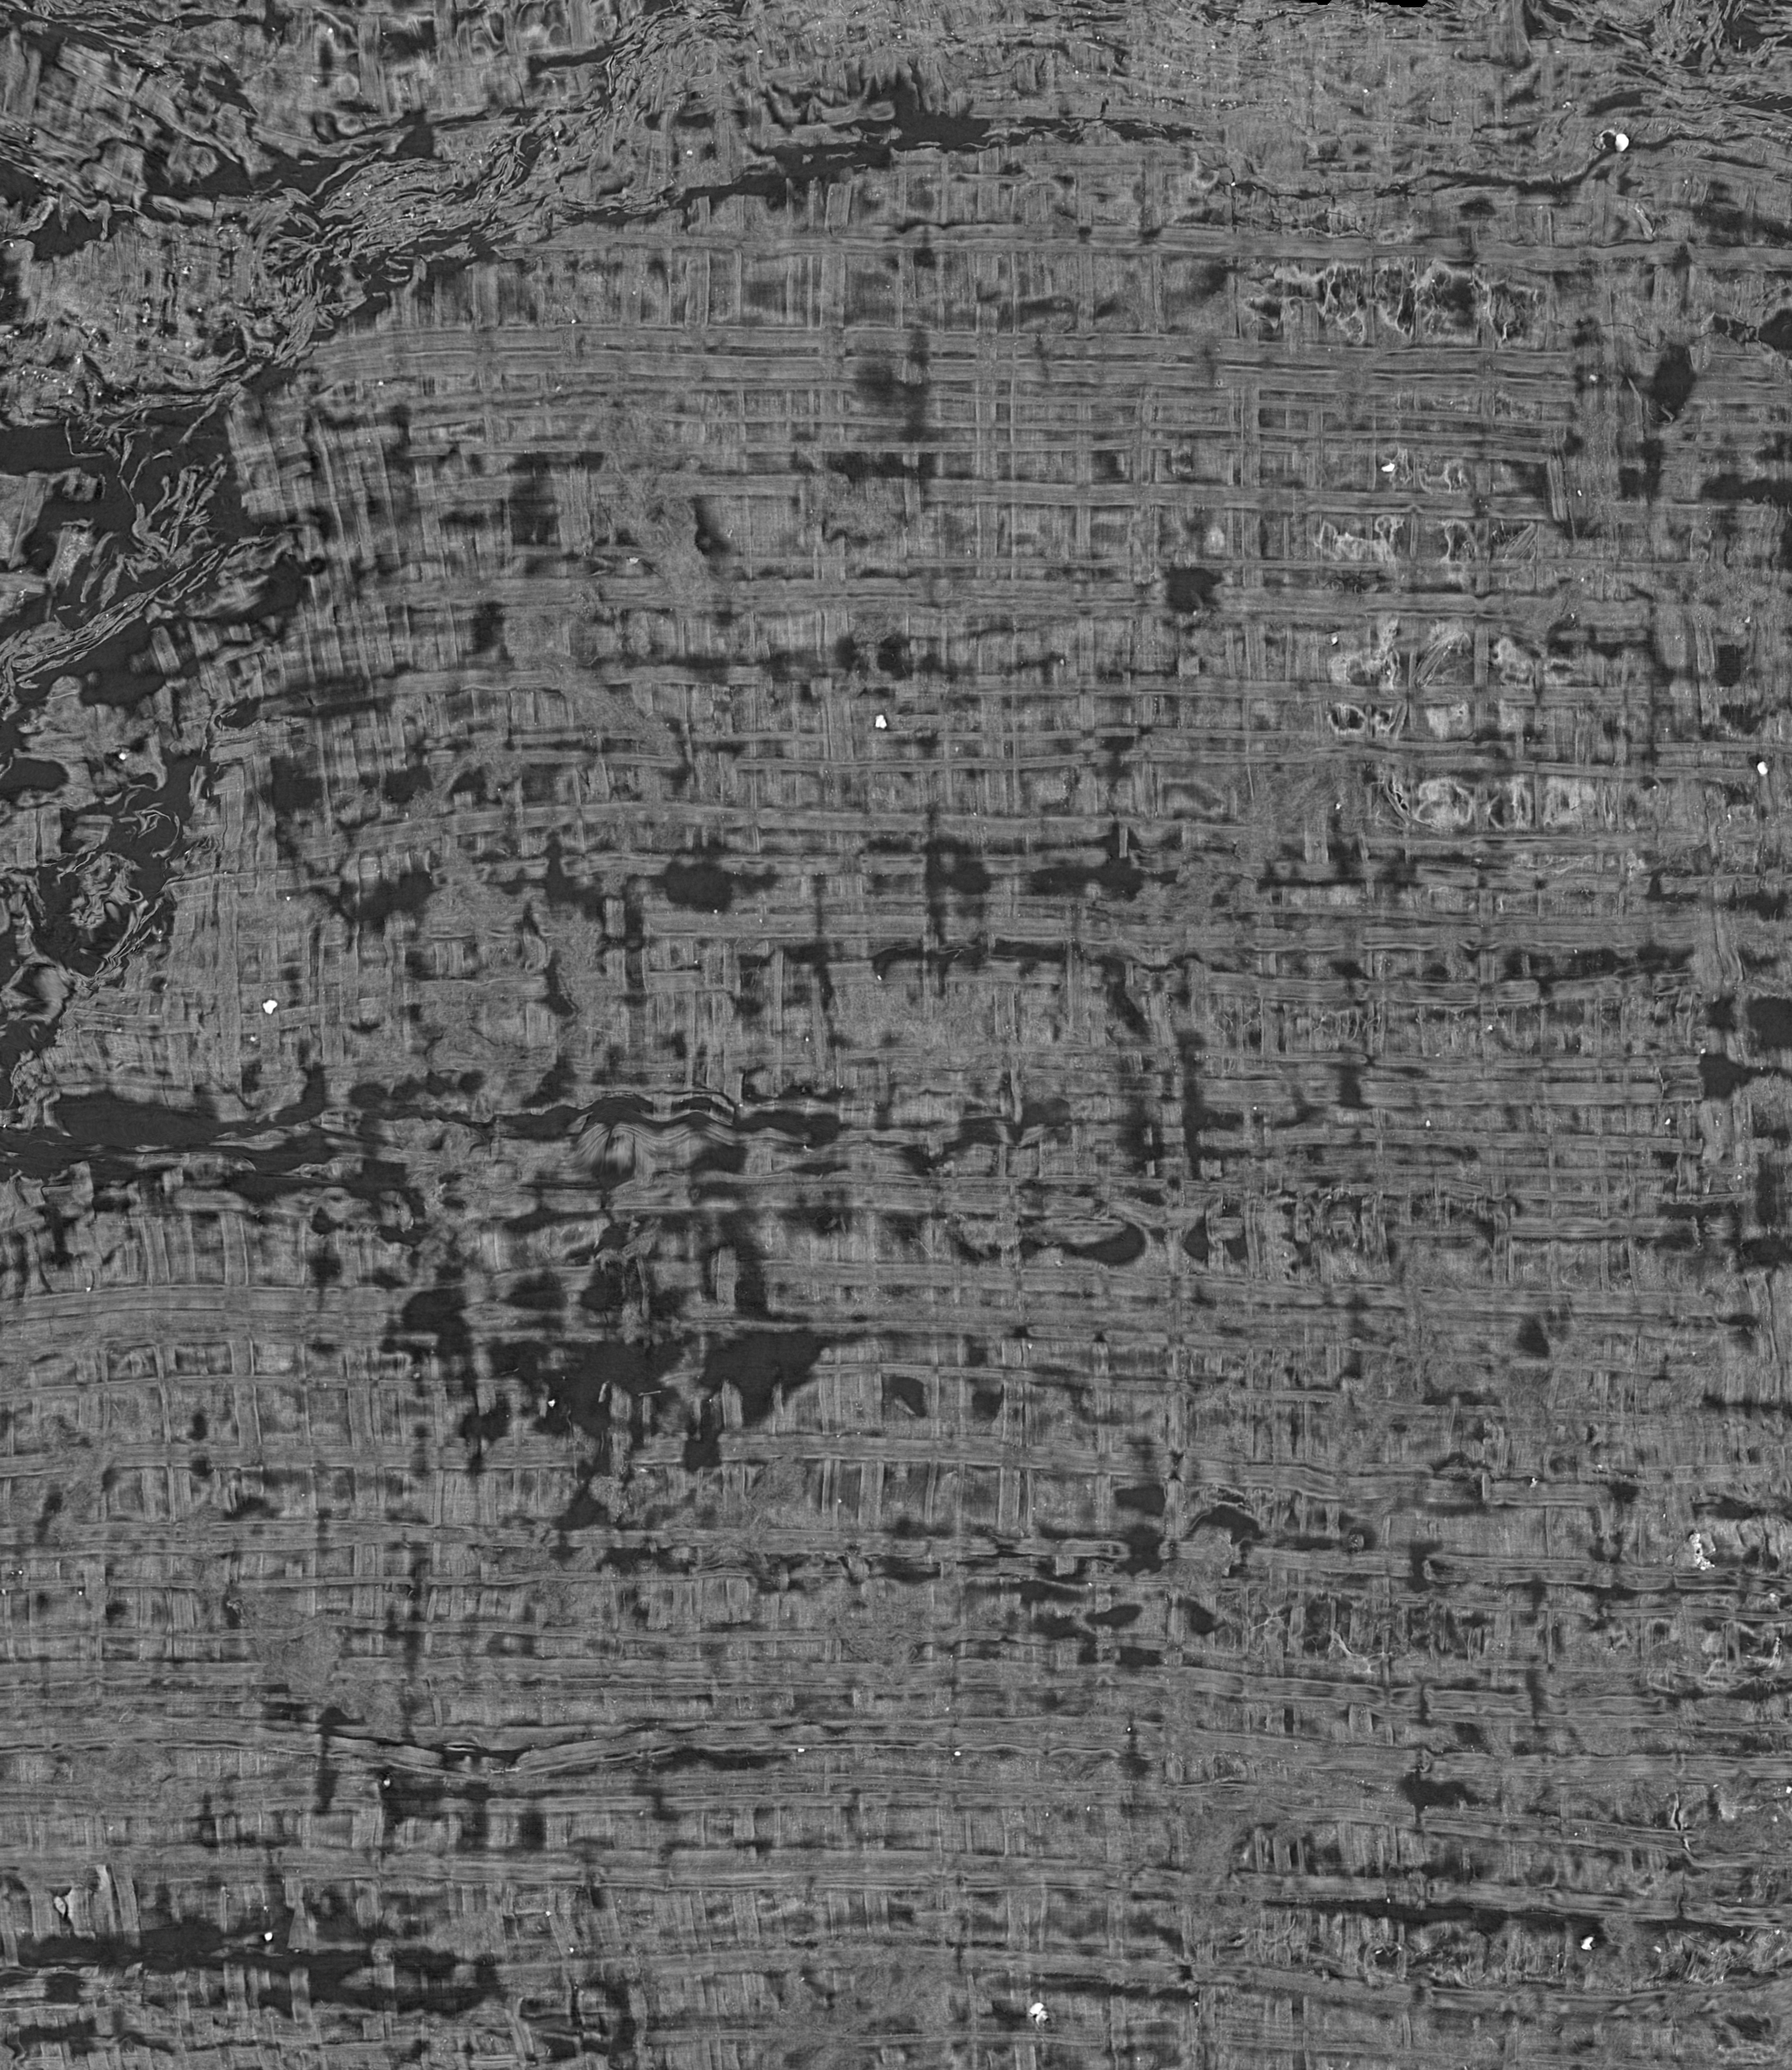
\includegraphics[width=122.48pt]{../figures/w060/w060_1_texture.png}}\end{minipage}\hspace{2pt}\begin{minipage}[t]{122.48pt}\centering\href{https://raw.githubusercontent.com/evilaliv3/vesuvius-challenge-pipeline/main/results/db27c806-rectina/src/figures/w060/w060_2_labels.png}{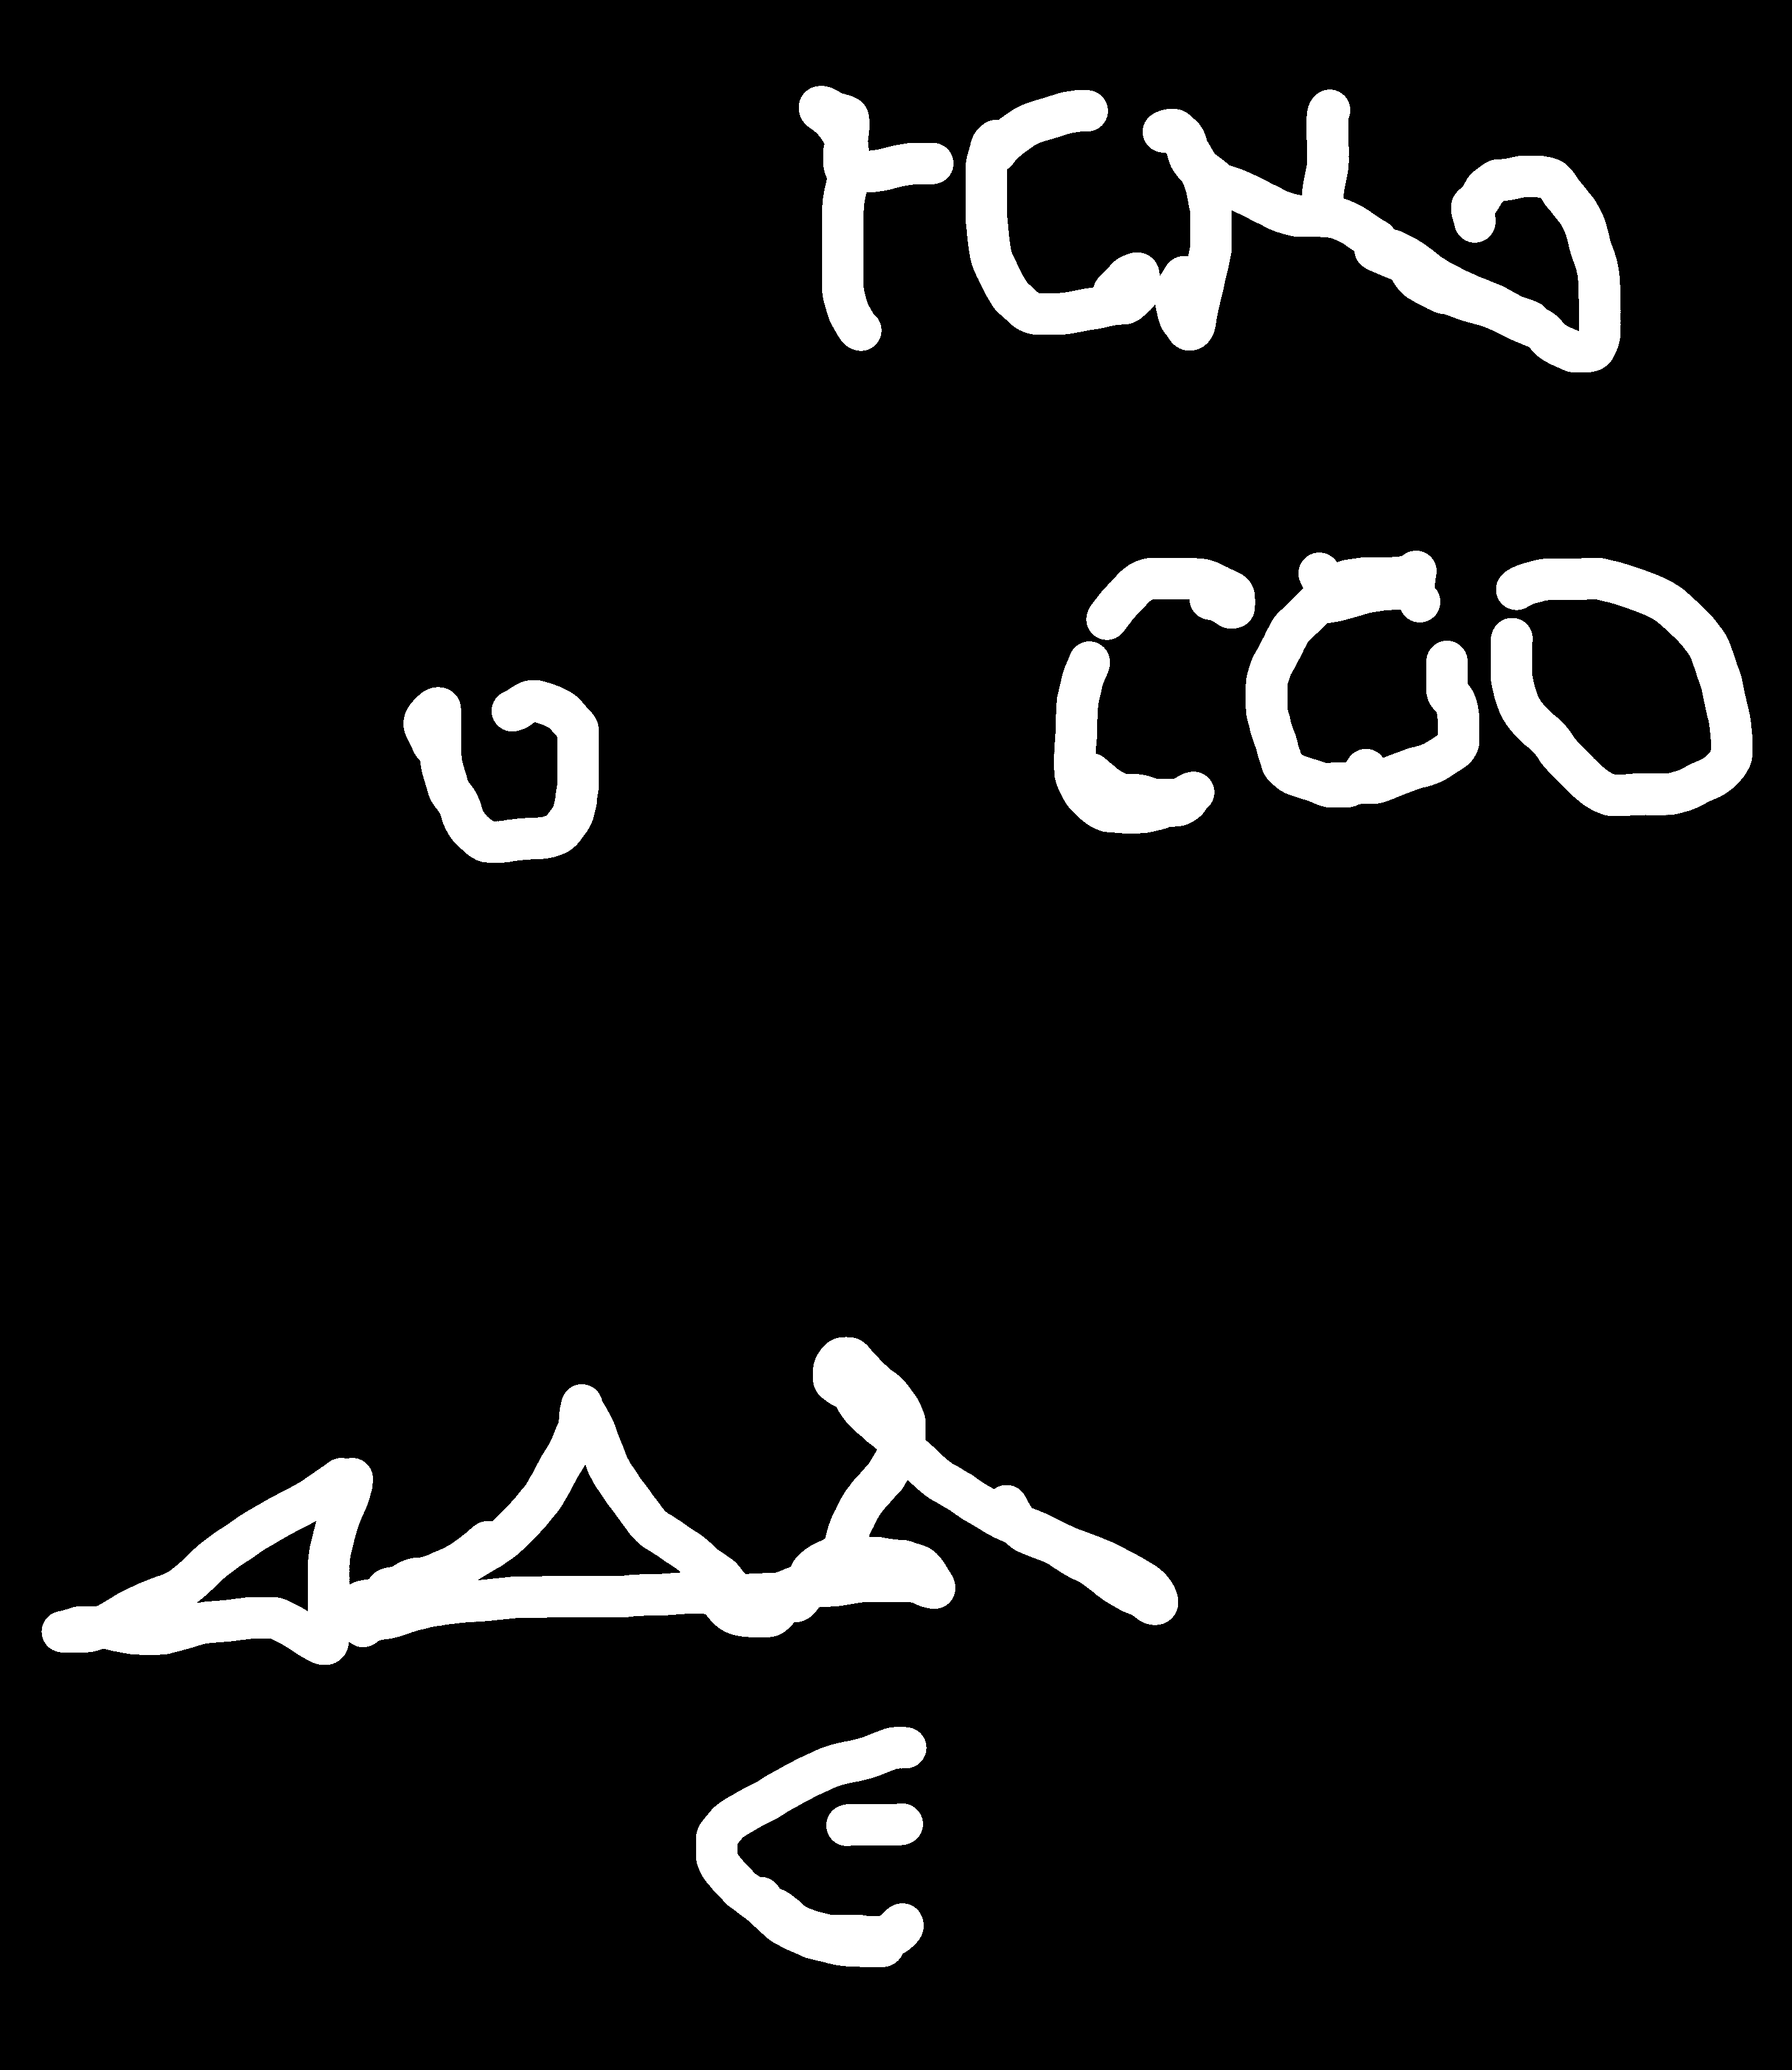
\includegraphics[width=122.48pt]{../figures/w060/w060_2_labels.png}}\end{minipage}}
\par\vspace{4pt}
\noindent\makebox[\columnwidth][c]{\begin{minipage}[t]{122.48pt}\centering\href{https://raw.githubusercontent.com/evilaliv3/vesuvius-challenge-pipeline/main/results/db27c806-rectina/src/figures/w060/w060_3_reader-v2.png}{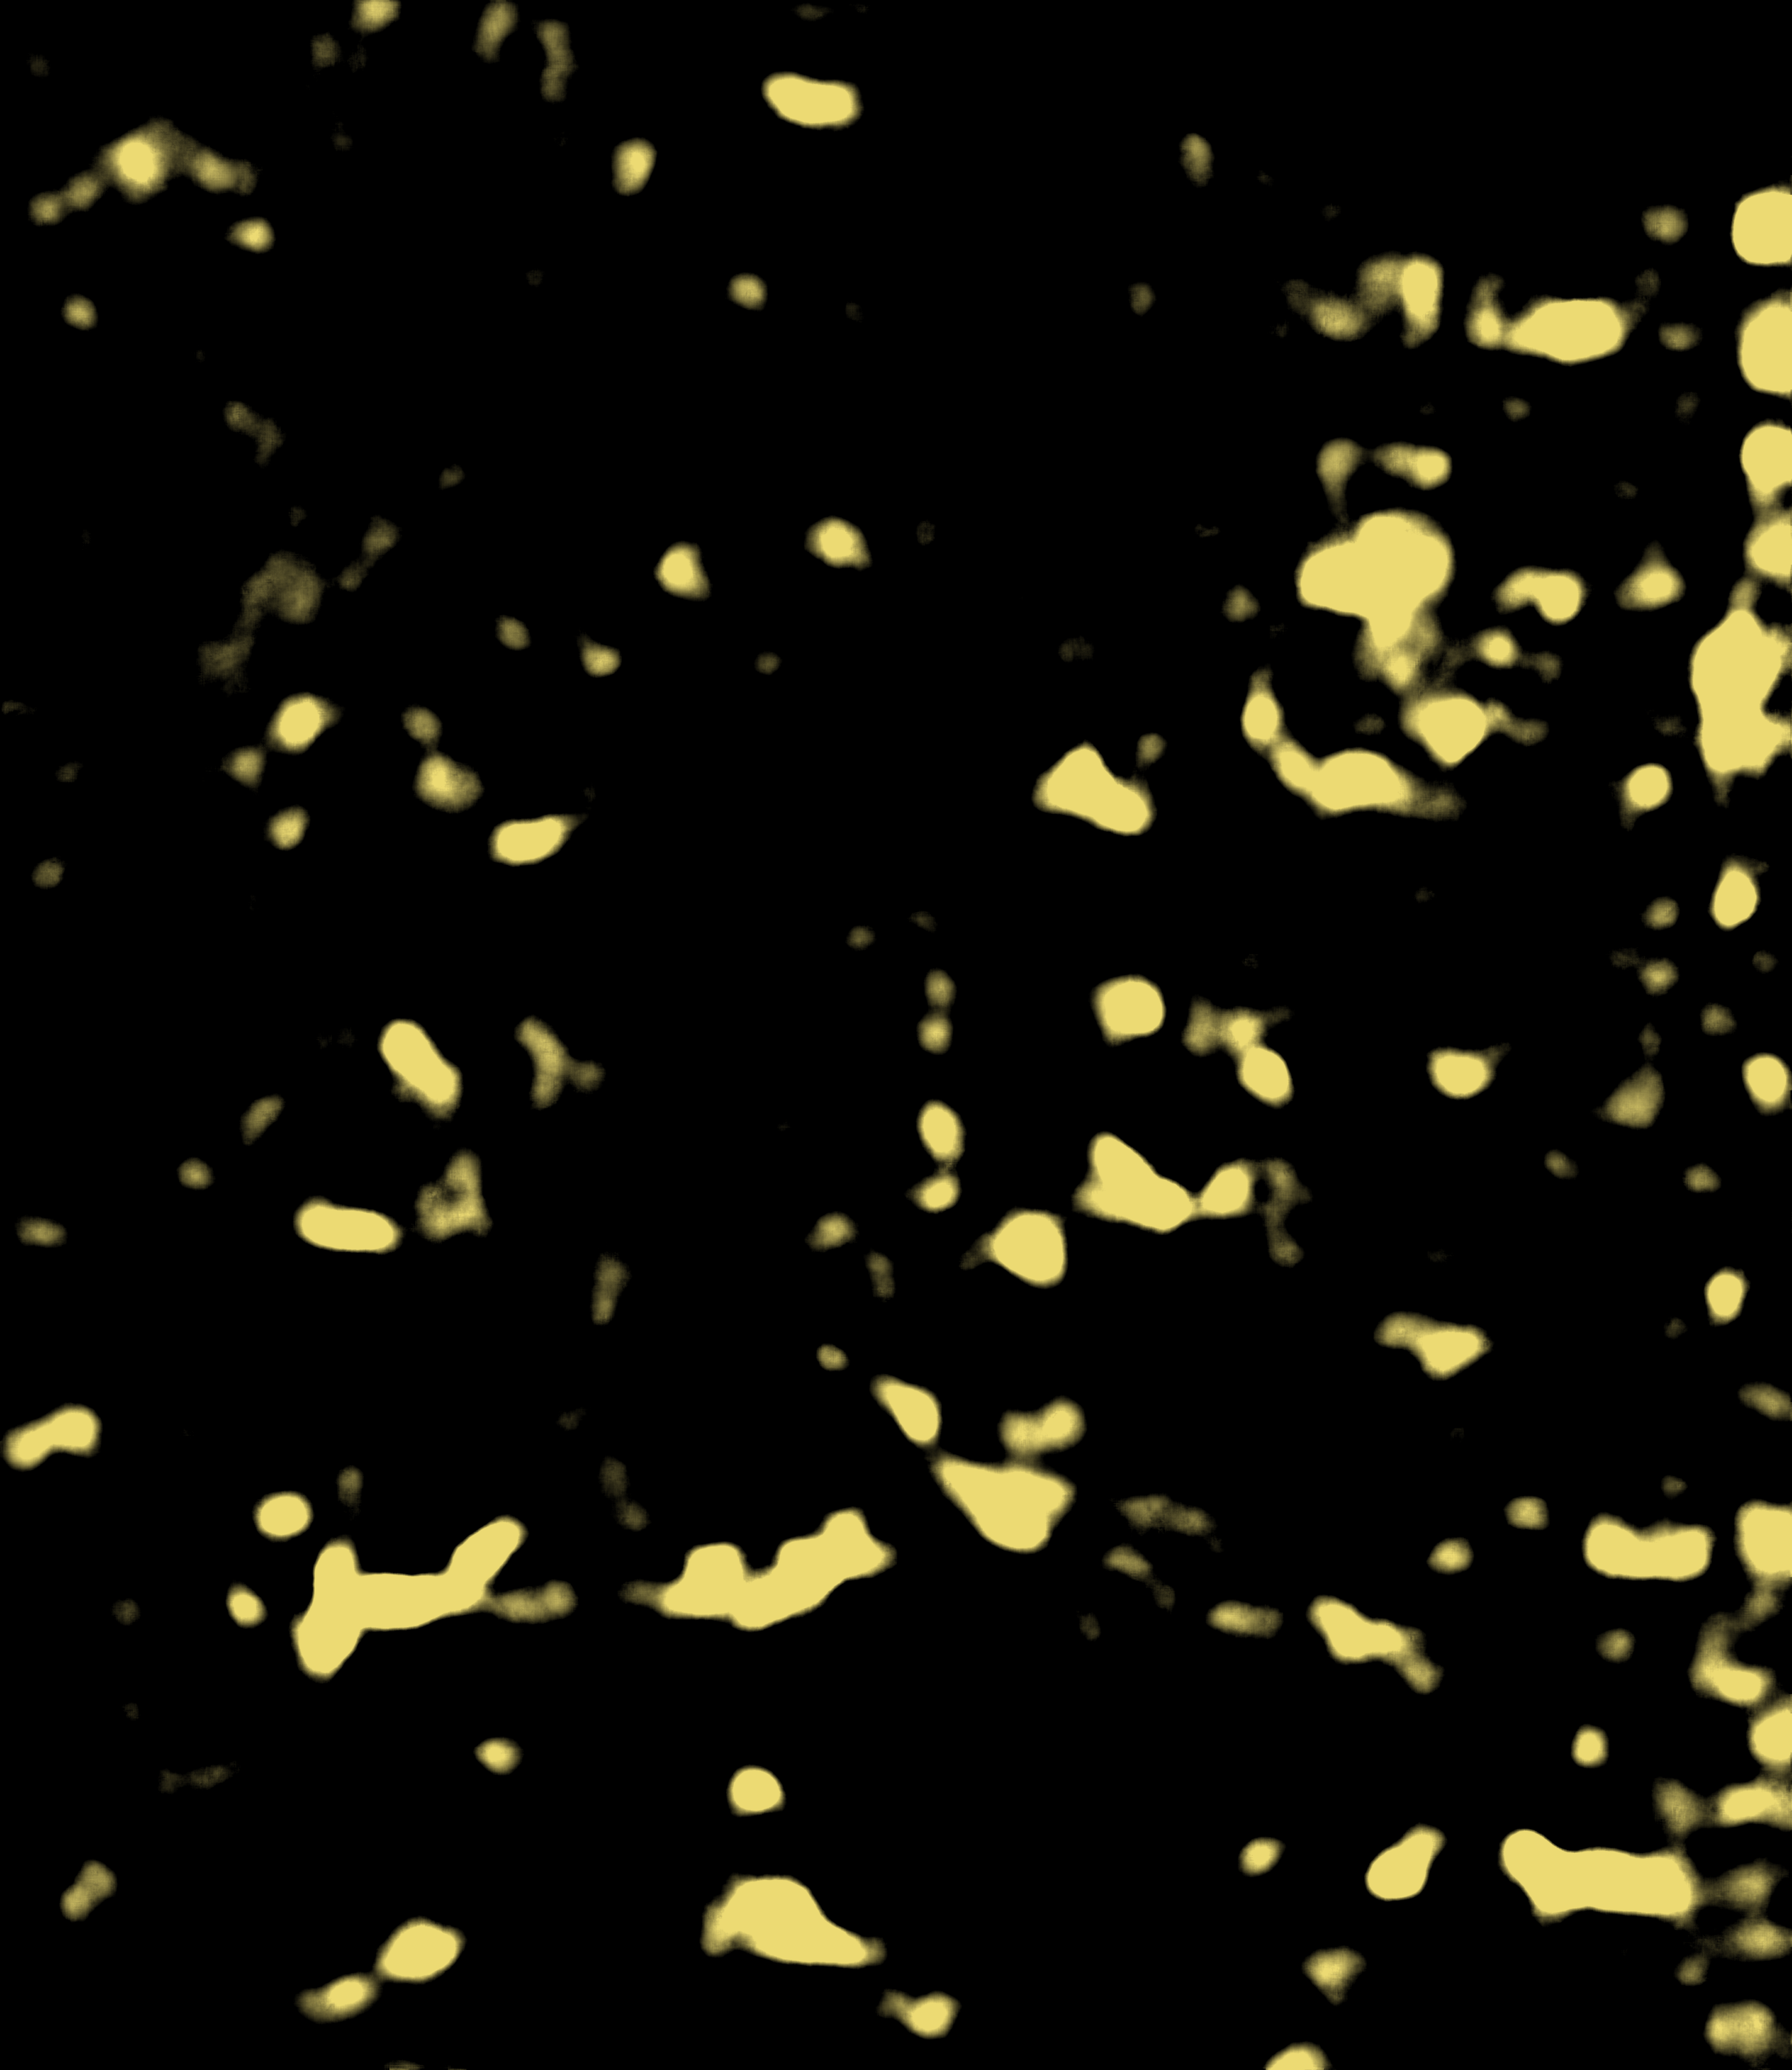
\includegraphics[width=122.48pt]{../figures/w060/w060_3_reader-v2.png}}\end{minipage}\hspace{2pt}\begin{minipage}[t]{122.48pt}\centering\href{https://raw.githubusercontent.com/evilaliv3/vesuvius-challenge-pipeline/main/results/db27c806-rectina/src/figures/w060/w060_5_rectina-m1.png}{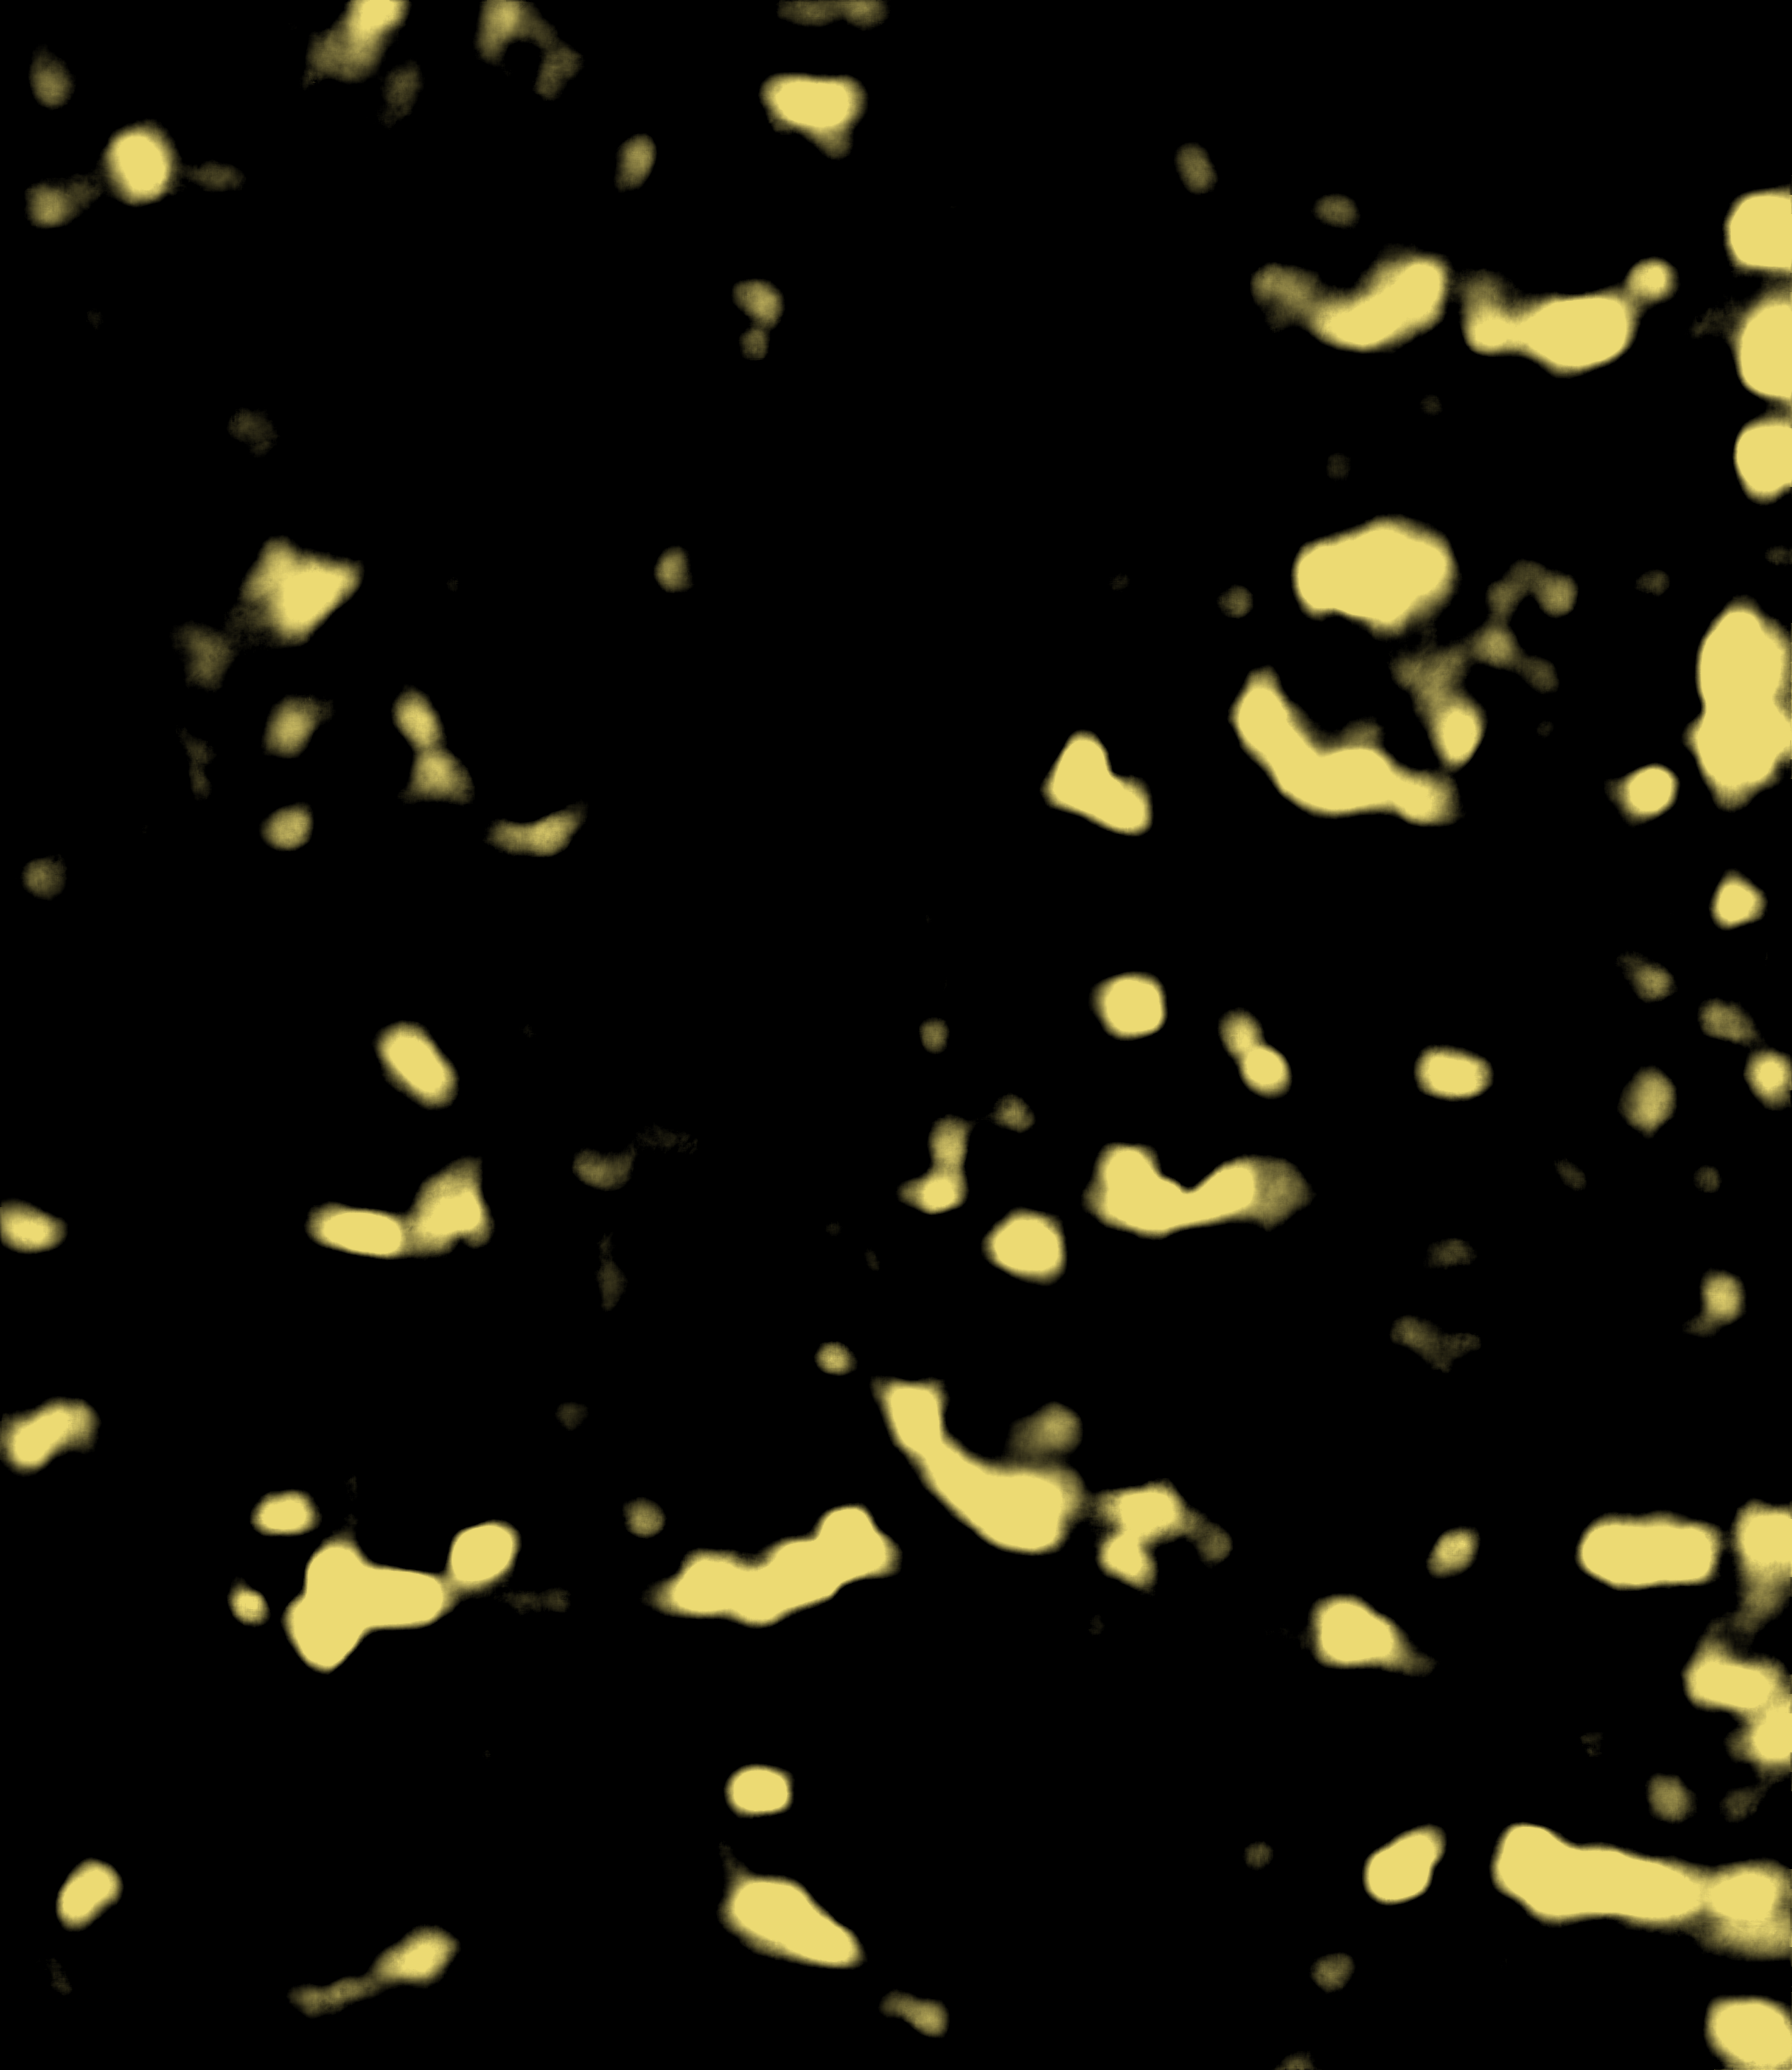
\includegraphics[width=122.48pt]{../figures/w060/w060_5_rectina-m1.png}}\end{minipage}}
\par\vspace{4pt}
\noindent\makebox[\columnwidth][c]{\begin{minipage}[t]{122.48pt}\centering\href{https://raw.githubusercontent.com/evilaliv3/vesuvius-challenge-pipeline/main/results/db27c806-rectina/src/figures/w060/w060_4_reader-v3.png}{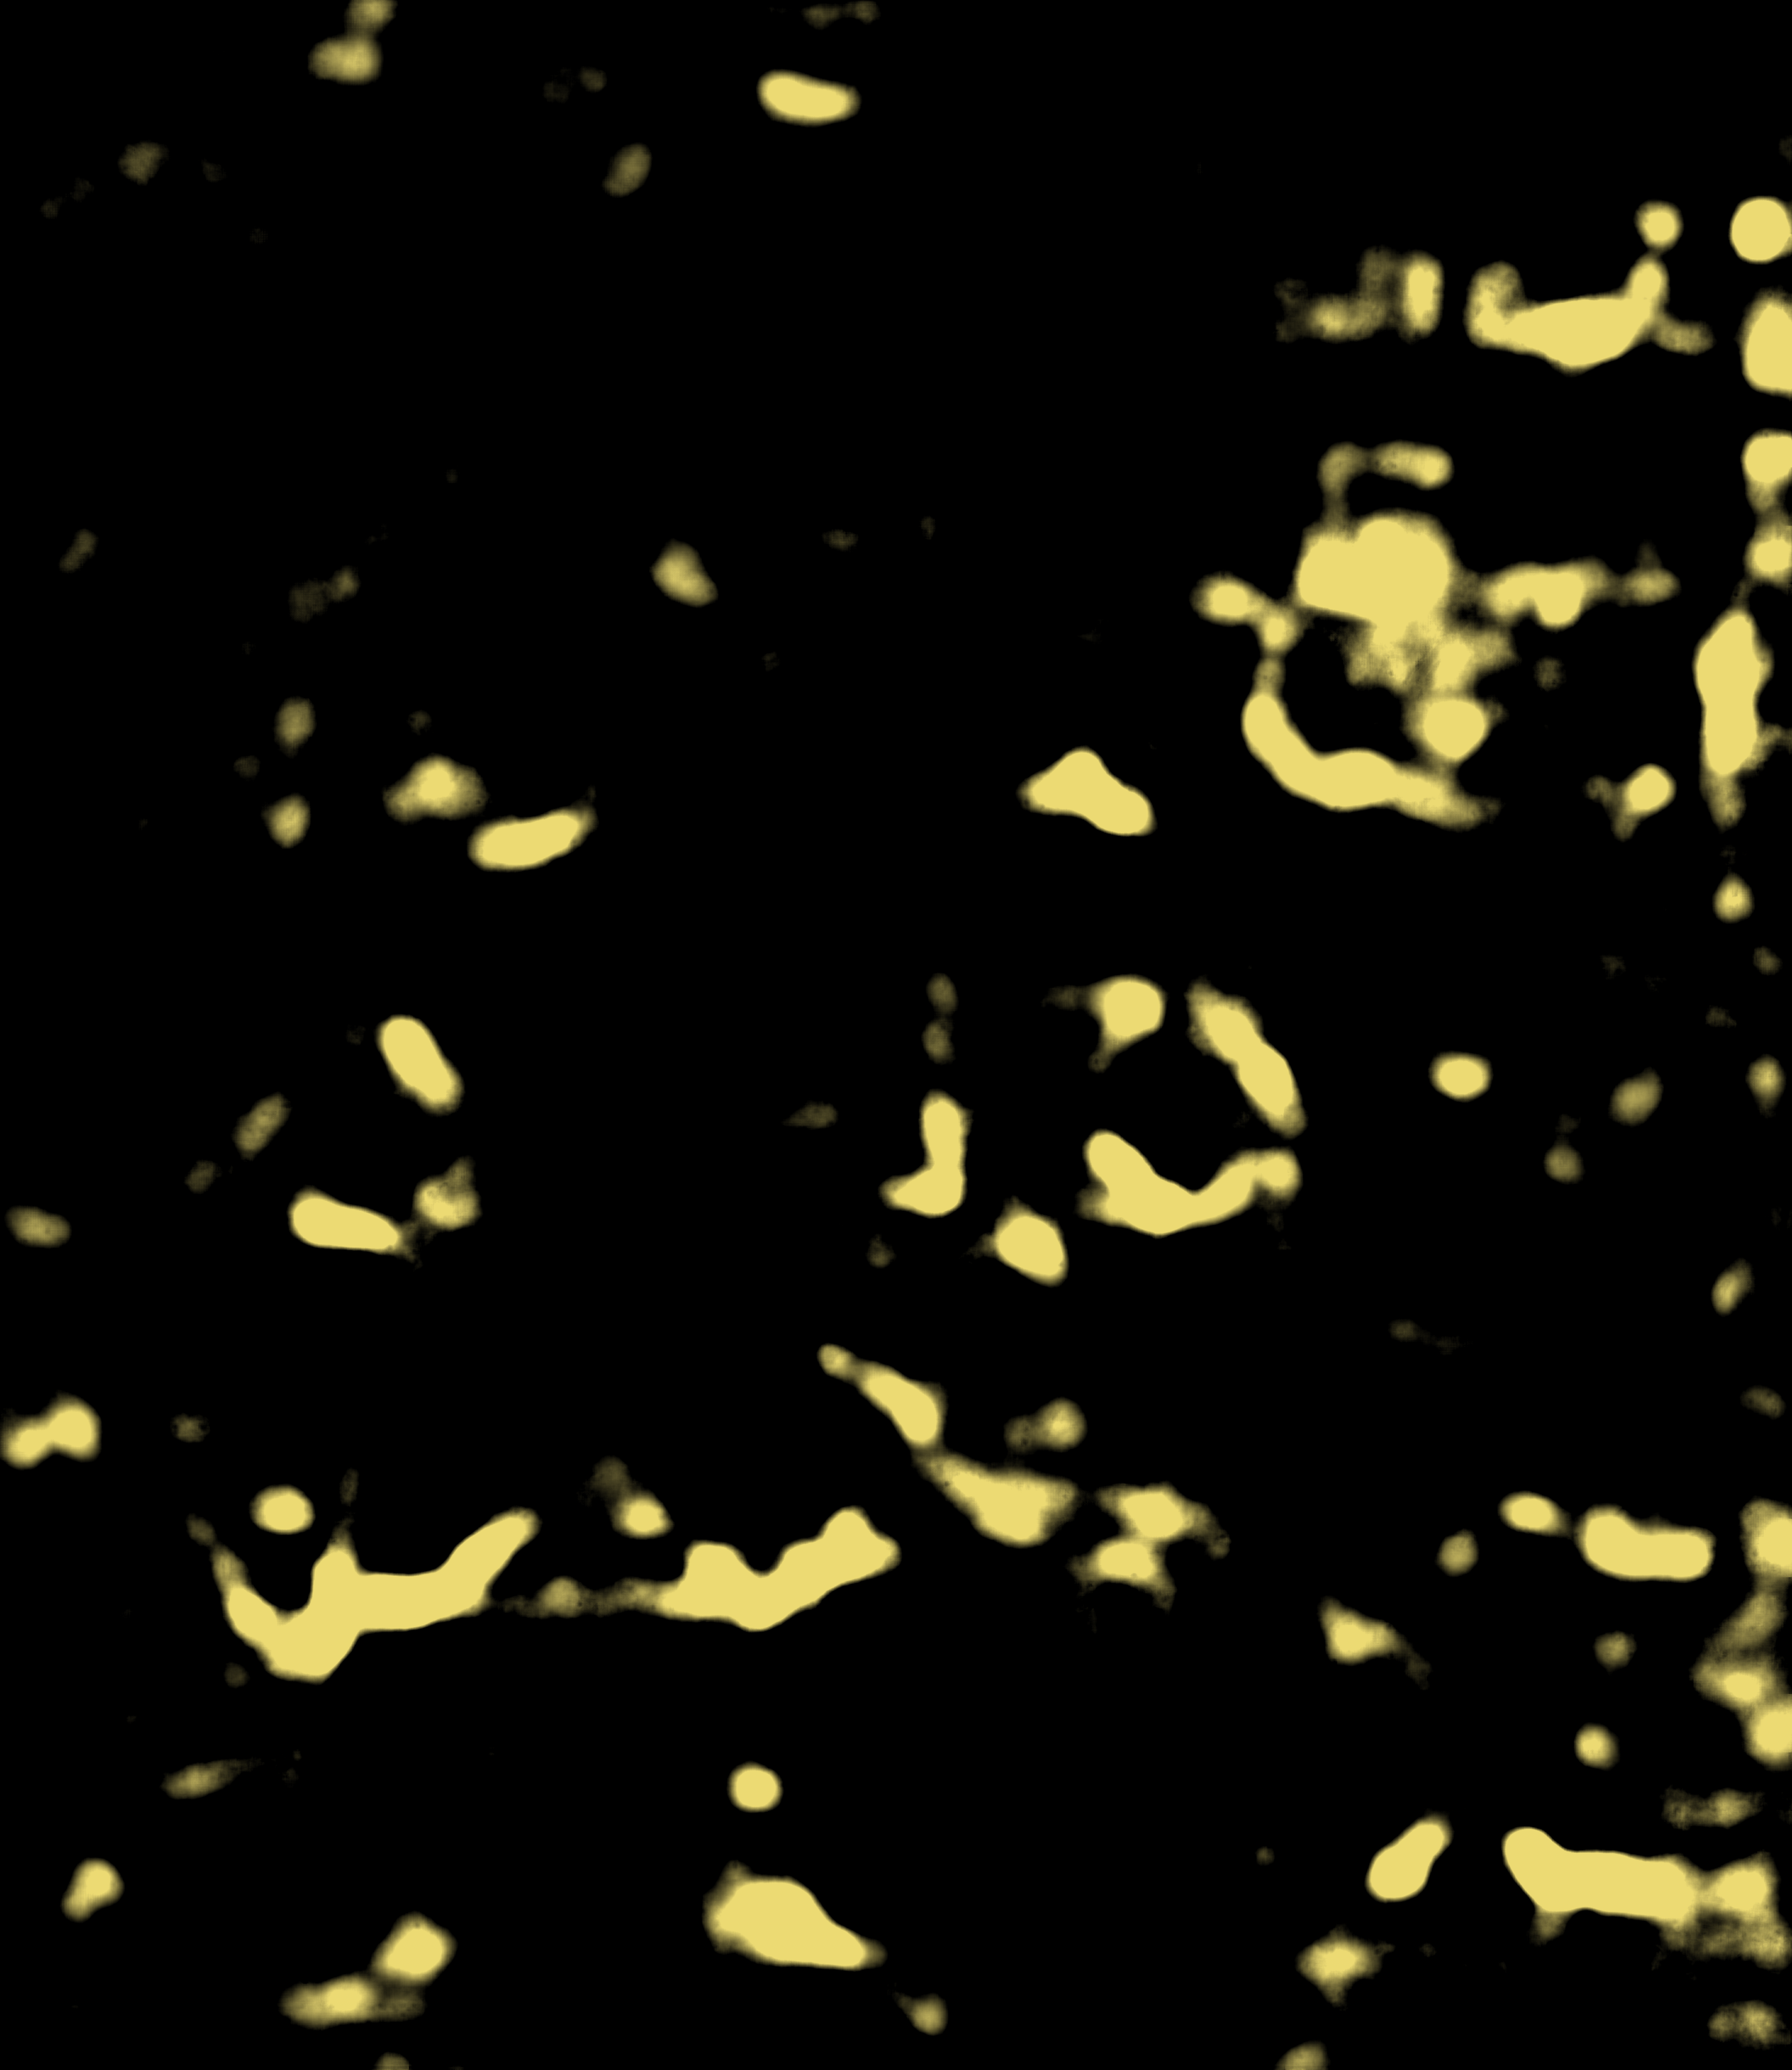
\includegraphics[width=122.48pt]{../figures/w060/w060_4_reader-v3.png}}\end{minipage}\hspace{2pt}\begin{minipage}[t]{122.48pt}\centering\href{https://raw.githubusercontent.com/evilaliv3/vesuvius-challenge-pipeline/main/results/db27c806-rectina/src/figures/w060/w060_6_rectina-m2.png}{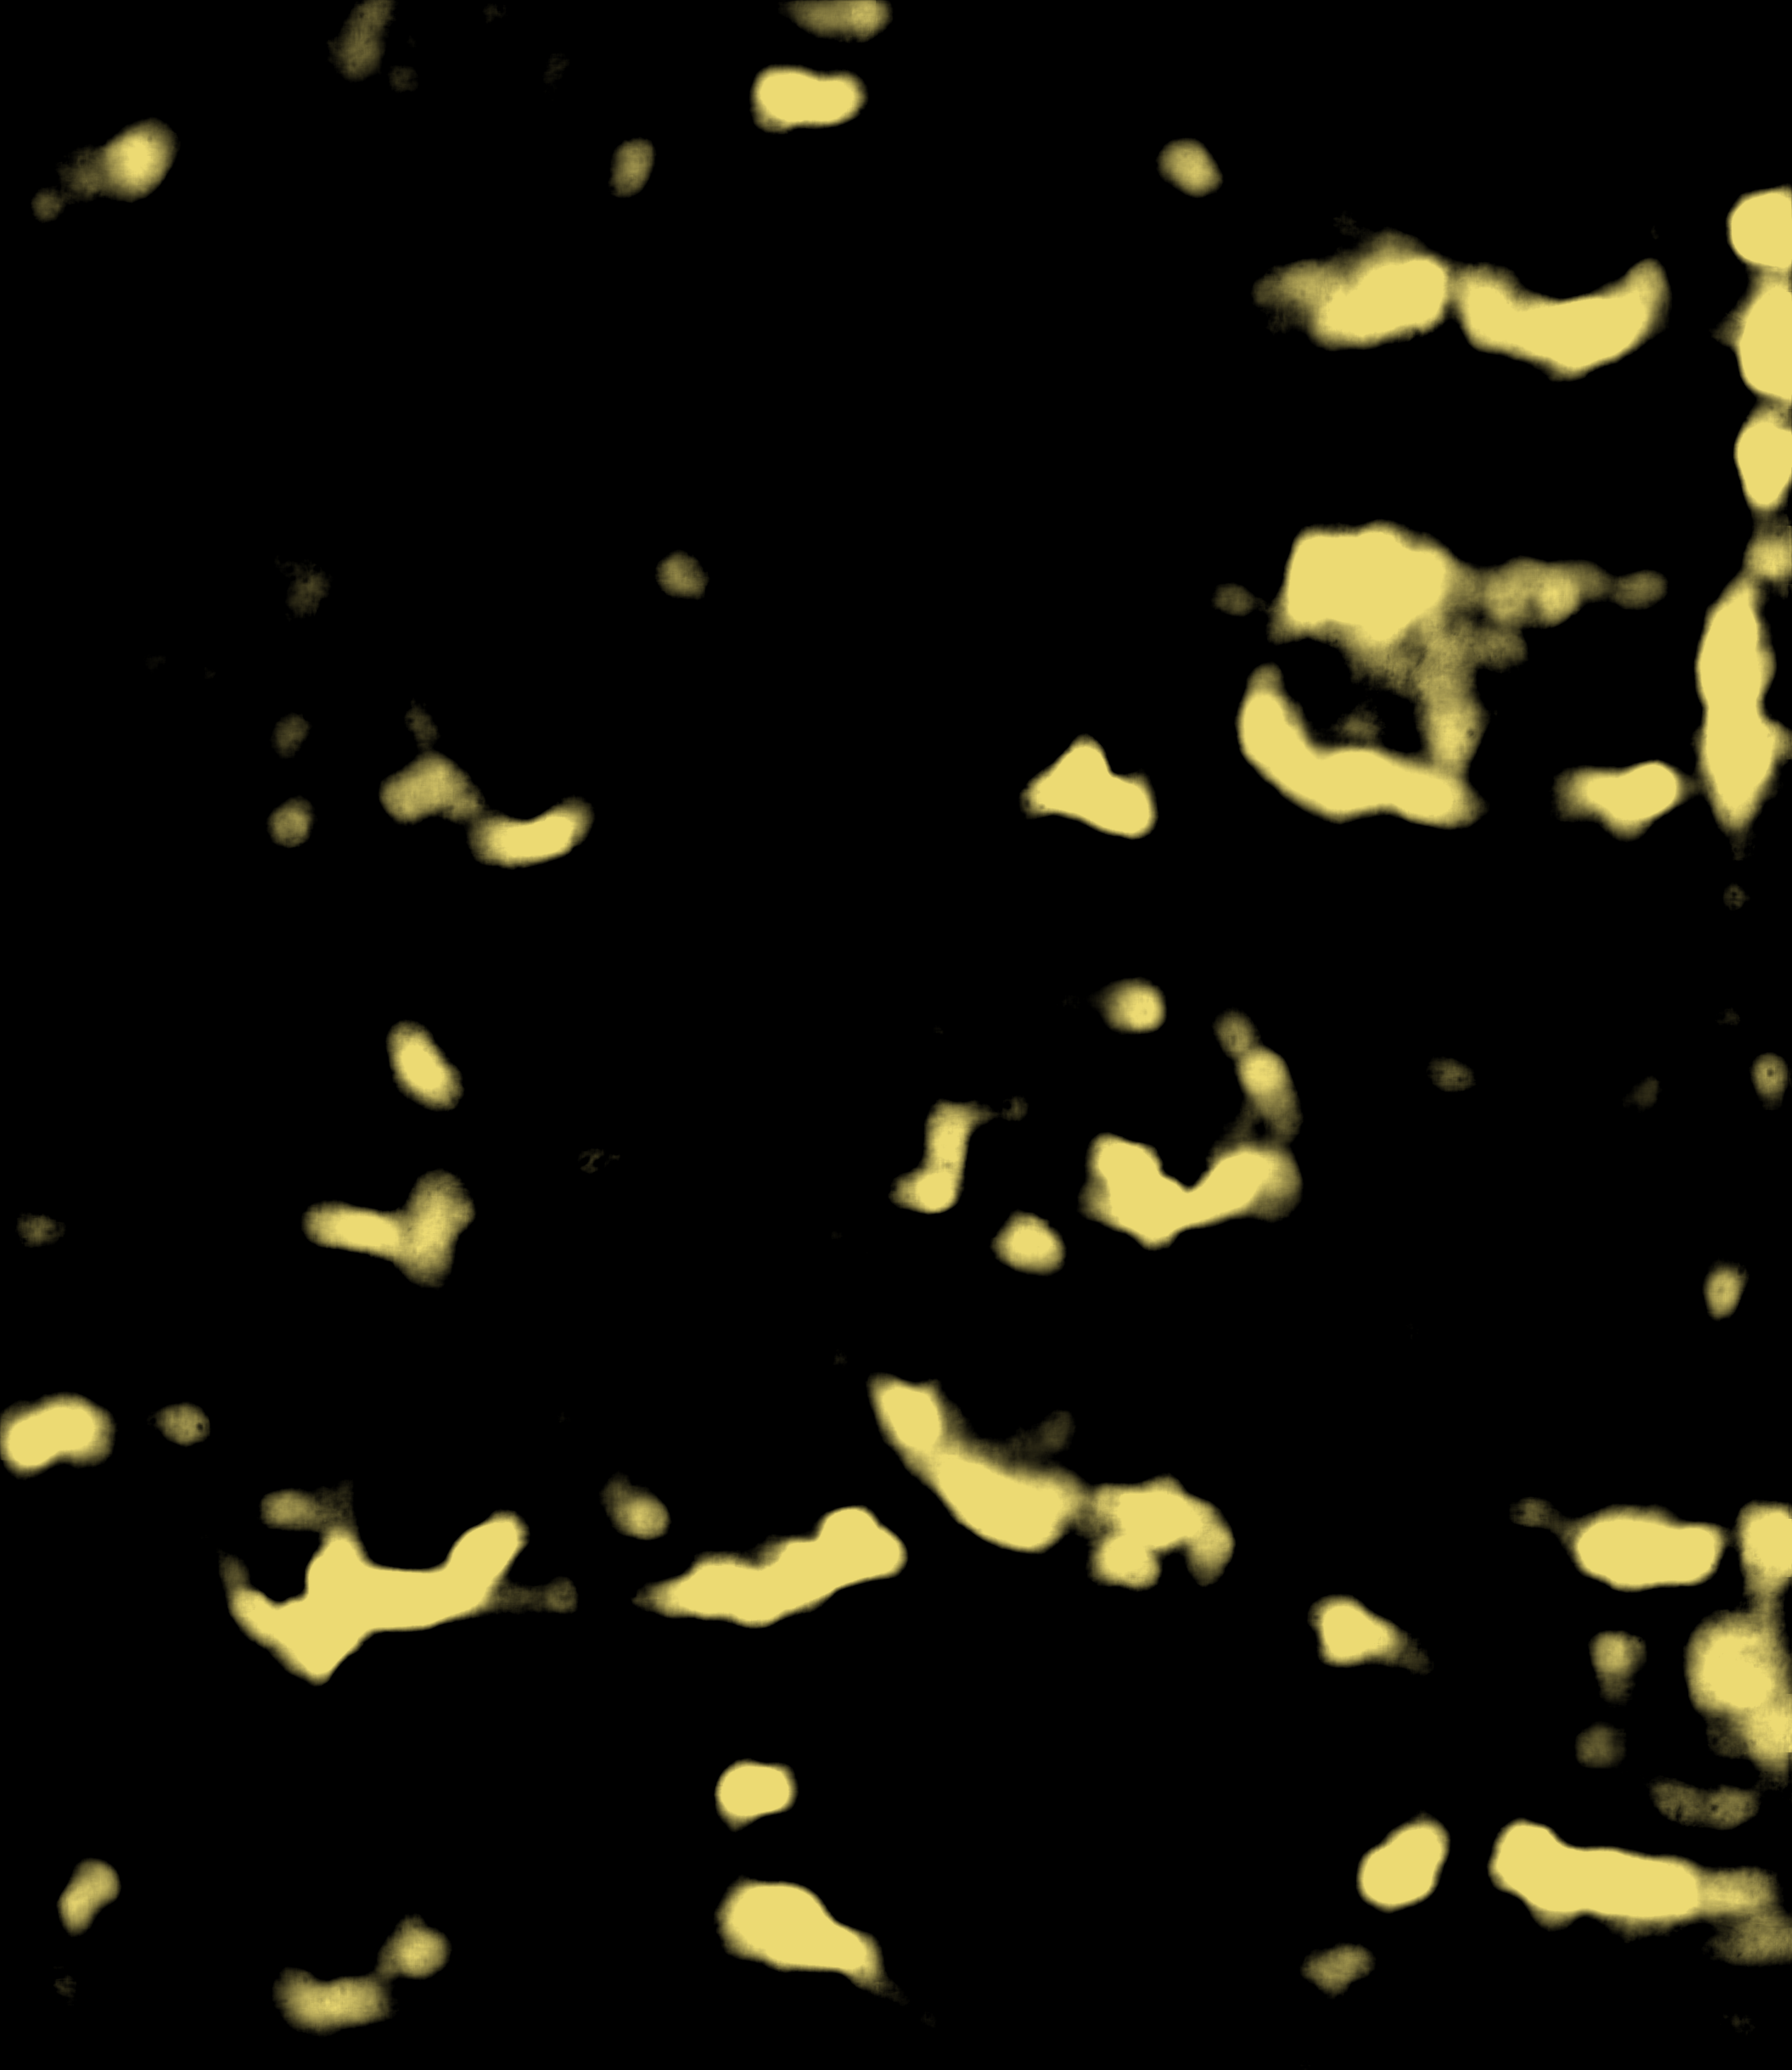
\includegraphics[width=122.48pt]{../figures/w060/w060_6_rectina-m2.png}}\end{minipage}}
\caption{Control unit 1447 w060, three rows of two panels. Row 1: left, Texture; right, Labels. Row 2: left, Reader v2; right, Rectina m1 (display windows: Reader v2 0.358837 to 0.460831 (ramp); Rectina m1 0.419819 to 0.580751 (ramp)). Row 3: left, Reader v3; right, Rectina m2 (display windows: Reader v3 0.381681 to 0.538574 (ramp); Rectina m2 0.465540 to 0.657352 (ramp)). Each map is stretched between its own percentiles. Reader and model stand side by side in the rows 2 and 3.}
\end{figure}
